\chapter{Princípios de Usabilidade presentes e avaliação por Heurísticas de Normam das Interfaces}
\label{chap:mockups}

\hspace{5mm} Neste capítulo serão ilustrados as mockups desenvolvidas para o projecto, bem como o resultado final/actual na aplicação web. Primeiro serão ilustradas as interfaces comuns, depois as interfaces dos Clientes e por último dos PTs. De seguida, serão também ilustrados alguns pormenores incorporados para uma melhor experiência dos utilizadores.

%--------------------------------------------------------------------------%

\section{Princípios/heurísticas genéricos(as) a todas as views}
\hspace{5mm} Inicialmente, apresentam-se os princípios/heurísticas genéricos/comuns a toda a interface, aqueles que ocorrem em praticamente todas as views.

\subsubsection{Princípios de usabilidade}
\begin{itemize}
    \item \textbf{Predictability}: de uma forma geral, todas as views cumprem este principio, onde o utilizador compreende o efeito das acções no sistema. 
    \item \textbf{Synthesizability}: de uma forma geral, todas as views, informam ao utilizador o estado a aplicação após acções do mesmo através de mensagens de erro, aviso e sucesso, que serão explicadas adiante.
    \item \textbf{Consistency}: de forma geral, a interface segue este princípio em todas as suas views, bem como em relação a todo sistema.
    \item \textbf{Customizability}: tamanho da janela adapta-se em computadores e tablets, no entanto, em smartphones seria necessário mais desenvolvimento, pois certas páginas não se adaptam correctamente.
\end{itemize}

\subsubsection{Heurísticas de Normam}
\begin{itemize}
    \item \textbf{Aesthetic and minimalist design}: tal como já foi referido anteriormente, toda a interface foi desenhada de forma simplista.
    \item \textbf{Visibility of system status}: em todas as interfaces existe uma nav bar que ajuda o utilizador a perceber onde se encontra. 
\end{itemize}

\section{Interfaces Comuns}
\label{sec:mockupscomuns}
\hspace{5mm} Nesta secção apresenta-se as interfaces que são comuns aos dois tipos de utilizadores do sistema, isto é, cliente e PT.

\subsection{Mensagens de sucesso, erro e aviso}
\label{subsec:sucesso}
\hspace{5mm} Visto que todas as views contém mensagens com a informação de erro, sucesso ou aviso sobre as acções do utilizador, acha-se importante começar a falar sobre as mesmas, pois aparecem em todas as views.

\subsubsection{Descrição da mensagem de sucesso}
\hspace{5mm} O alerta de Sucesso é utilizado para informar os utilizadores quando as suas acções são realizadas com sucesso mas não é óbvio para o utilizador que estas foram realizadas com sucesso.

\begin{figure}[H]
    \centering
    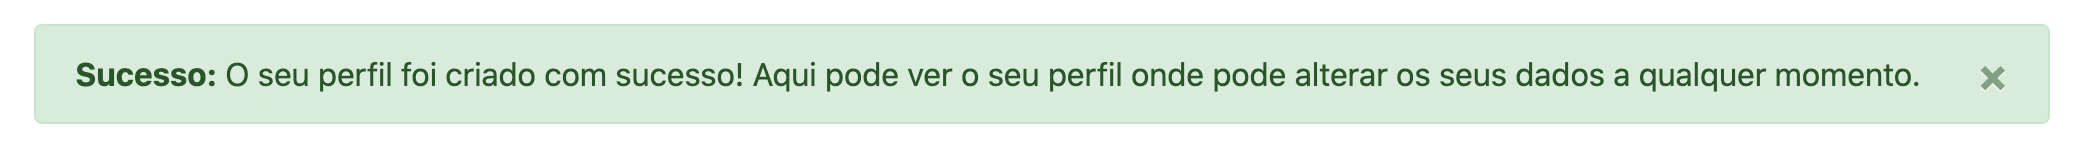
\includegraphics[scale=0.45]{images/alerts/alerta_sucesso.png}
    \caption{Alerta de Sucesso.}
    \label{fig:alertasucesso}
\end{figure}

\subsubsection{Descrição da mensagem de aviso}
\hspace{5mm} O alerta de Aviso é utilizado quando ocorre algum problema, no entanto não impede a continuidade da acção.

\begin{figure}[H]
    \centering
    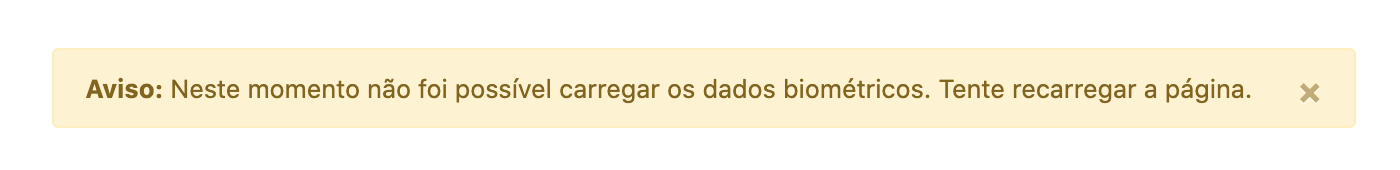
\includegraphics[scale=0.65]{images/alerts/alerta_aviso.png}
    \caption{Alerta de Aviso.}
    \label{fig:alertaaviso}
\end{figure}

\subsubsection{Descrição da mensagem de erro}
\hspace{5mm} O alerta de Erro é utilizado quando o utilizador introduz dados inválidos ou quando existem erros internos dos servidores.

\begin{figure}[H]
    \centering
    
\includegraphics[scale=0.45]{images/alerts/alerta_erro.png}
    \caption{Alerta de Erro.}
    \label{fig:alertaerro}
\end{figure}

\subsubsection{Princípios de usabilidade}
\begin{itemize}
    \item \textbf{Synthesizability}: as mensagens de erro, sucesso ou aviso informam o utilizador do estado do sistema. Desta forma, \textbf{visto que as mensagens ocorrem em todas as páginas, pode-se afirmar que este princípio também}.
    \item \textbf{Generability}: visto que é genérico a todas as views, ou seja, igual em todas as views, mudando apenas o conteúdo da mensagem.
    \item \textbf{Consistency}: tal com foi referido, todas as views implementam as mensagens de erros, sucesso e avisos, logo, torna-se consistente.
\end{itemize}

\subsubsection{Heurísticas de Normam}
\begin{itemize}
    \item \textbf{Visibility of system status}: as mensagens mantém o utilizador informado sobre o que está a acontecer, ou o estado da aplicação.
    \item \textbf{Consistency and standards e Aesthetic and minimalist design}: o design usado para as mensagens de erro são \textbf{minimalista} e \textbf{comum}/\textbf{padrão}, tal como se pode ver nas imagens \ref{fig:alertasucesso}, \ref{fig:alertaaviso} e \ref{fig:alertaerro}.
    \item \textbf{Help users recognize and recover from errors}: as mensagens de erro são bastante informativas na medida do necessário em informar o que aconteceu, bem como dar uma possível solução para o problema ou alternativa.
\end{itemize}

\subsection{Login}
\label{subsec:login}

\subsubsection{Descrição}
\hspace{5mm} De forma a facilitar a autenticação para o utilizador o login é comum aos dois tipos de utilizadores da plataforma, sendo que estes apenas precisam de introduzir as suas credenciais. Podem ainda seleccionar "Registar Cliente" ou "Registar Personal Trainer" caso sejam novos no sistema.

\begin{figure}[H]
    \centering
    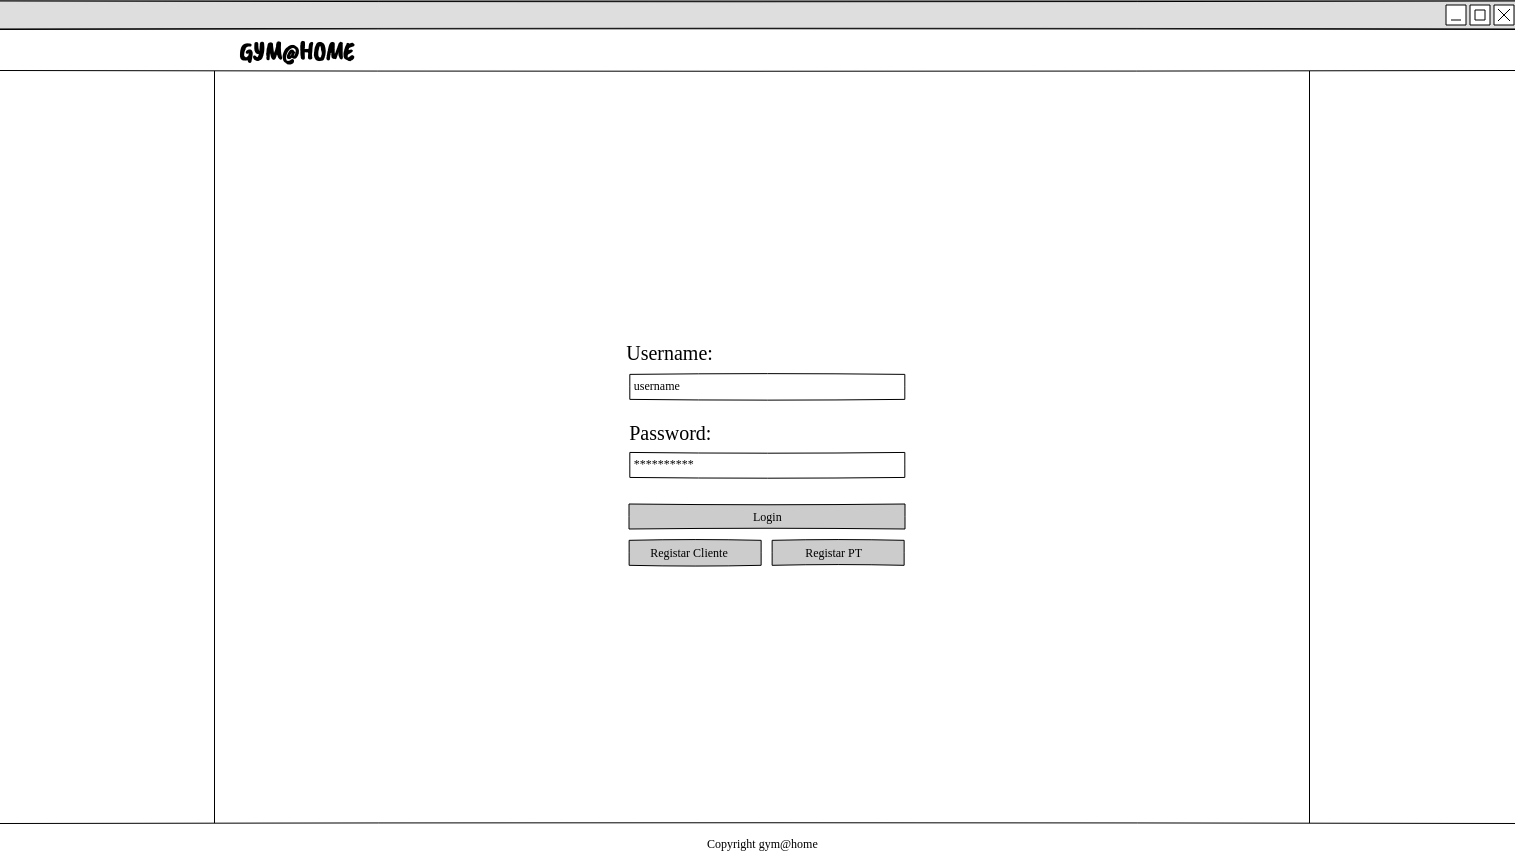
\includegraphics[scale=0.25]{images/mockups/login.png}
    \caption{Mockup Login.}
    \label{fig:mockuplogin}
\end{figure}

\begin{figure}[H]
    \centering
    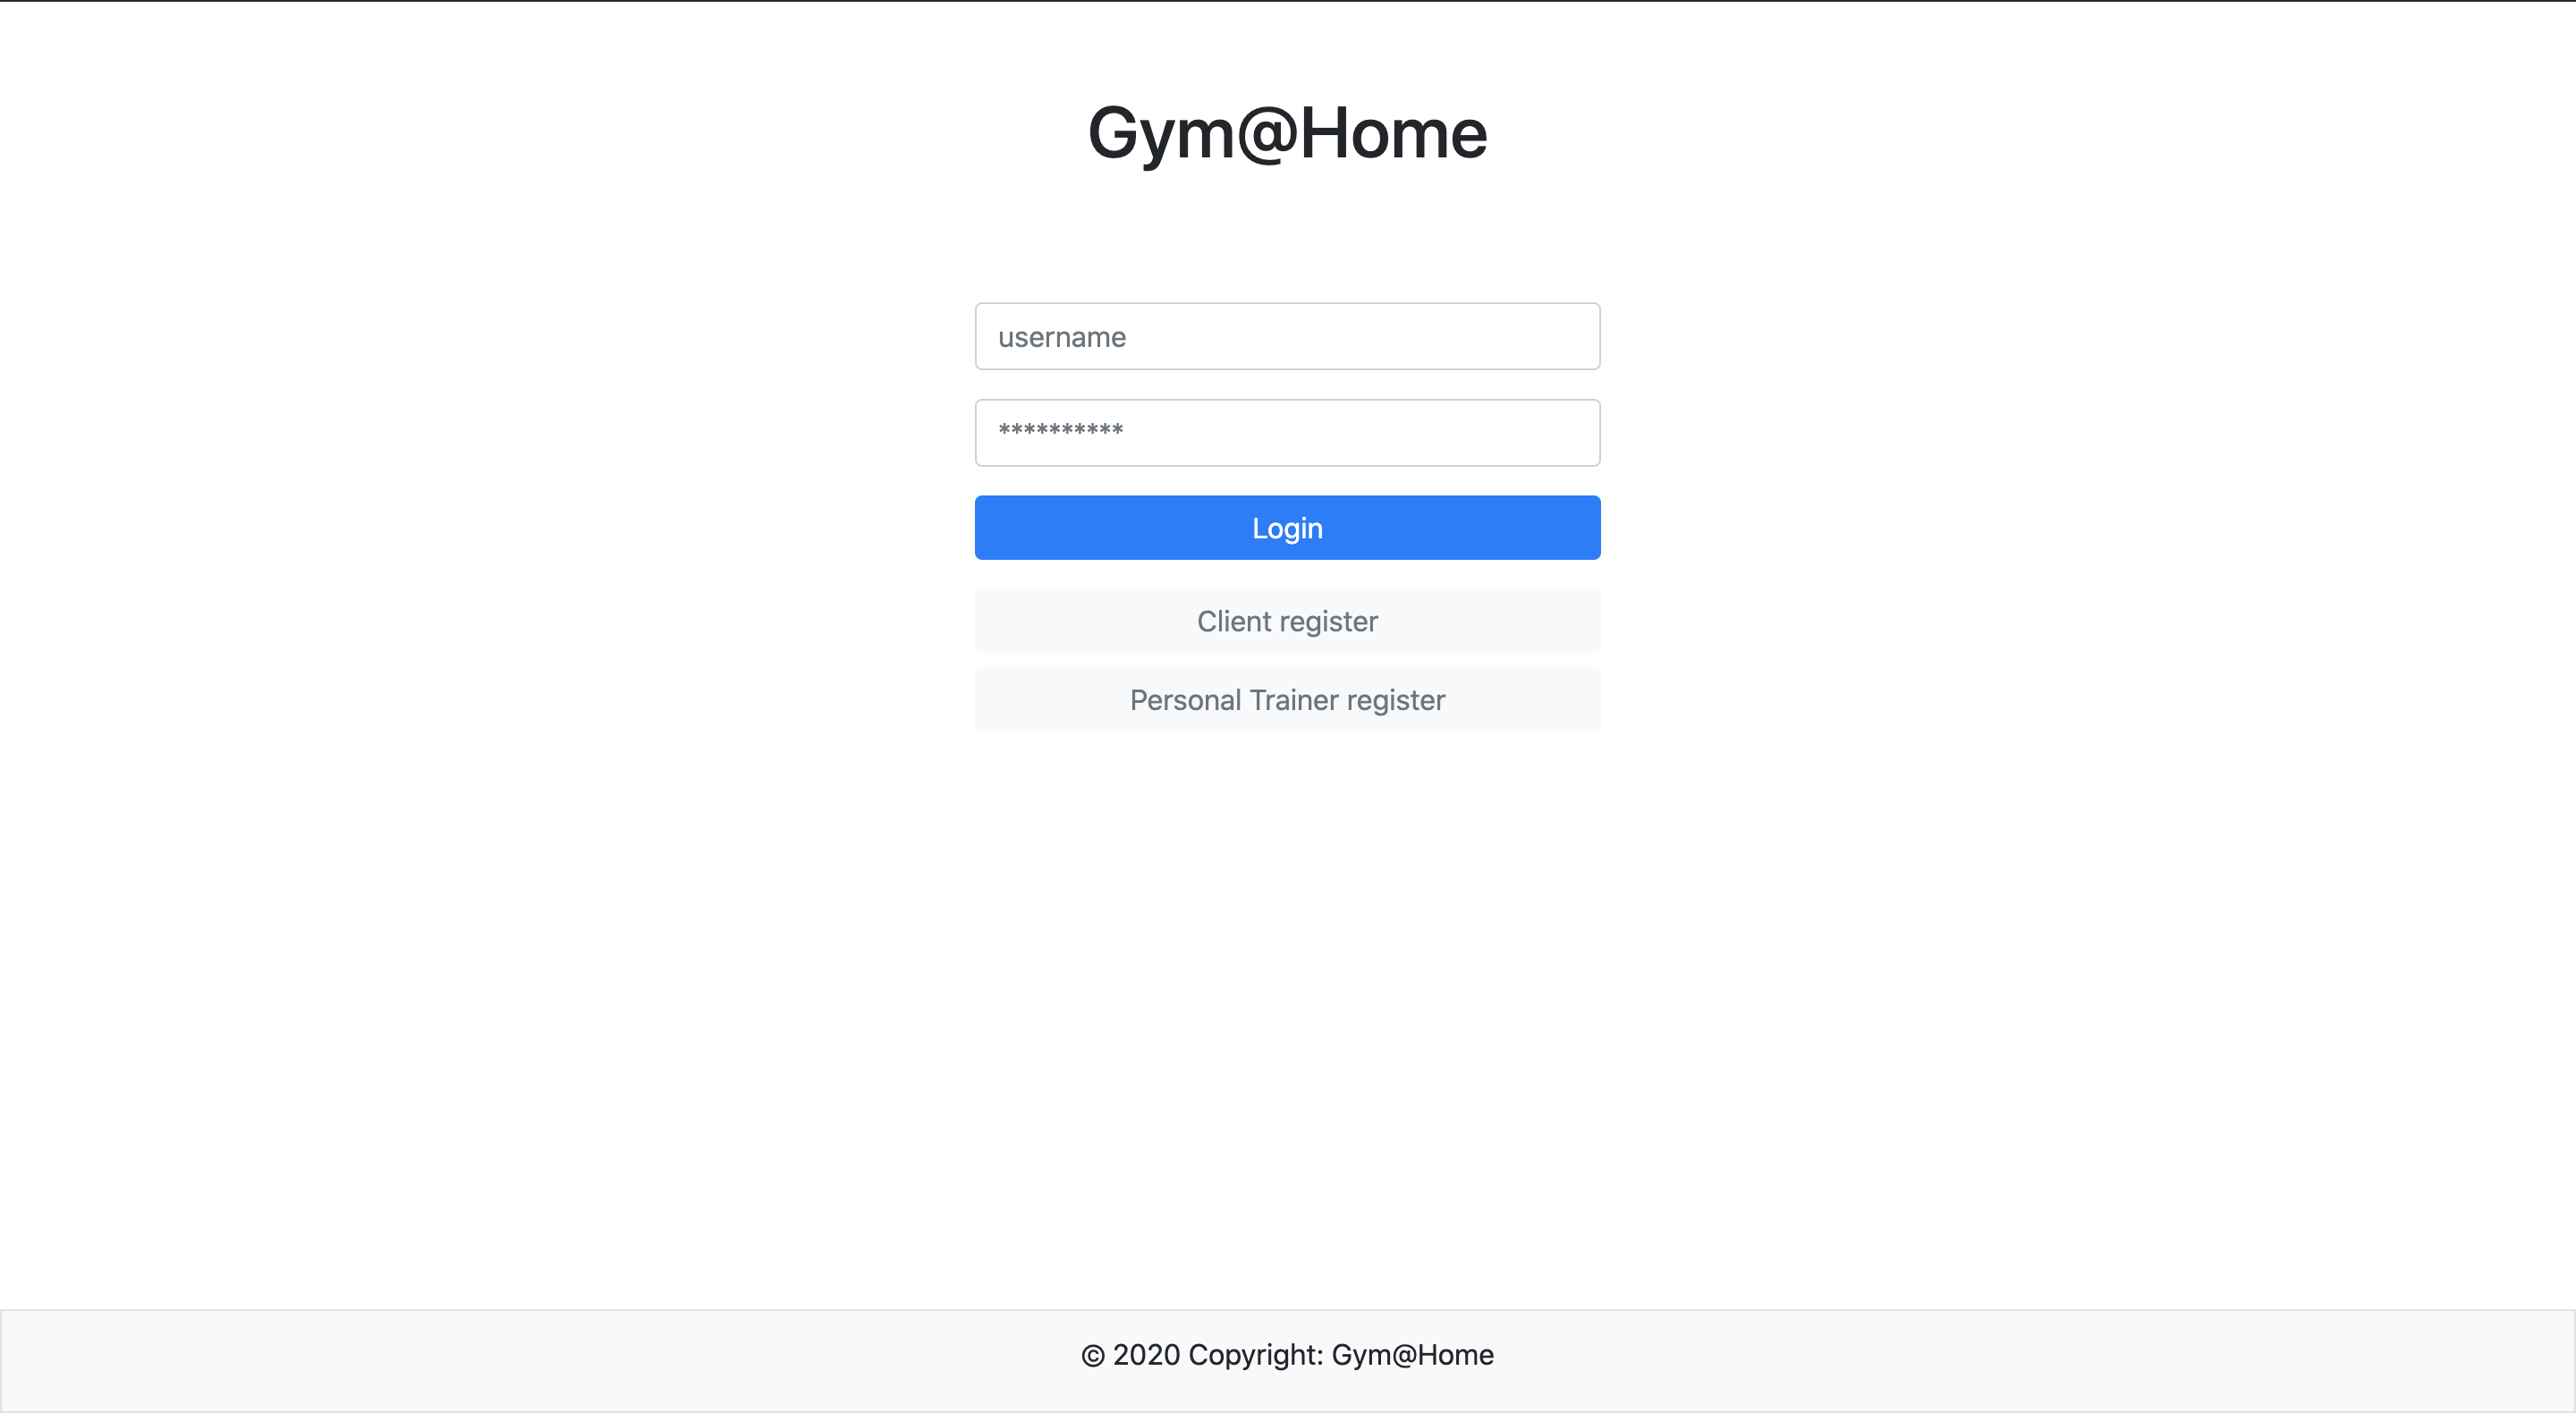
\includegraphics[scale=0.25]{images/interfaces/login.png}
    \caption{Interface Login.}
    \label{fig:interfacelogin}
\end{figure}

\subsubsection{Princípios de usabilidade}
\begin{itemize}
    \item \textbf{Predictability}: o utilizador percebe o efeito das acções, neste caso, fazer o login ou registar-se.
    \item \textbf{Familiarity}: seguiu-se o padrão de desenho de logins presente normalmente em maior parte das aplicações web.
    \item \textbf{Consistency}: bastante semelhante ao anterior, na medida em que o princípio da consistência torna-se mais abrangente.
\end{itemize}

\subsubsection{Heurísticas de Normam}
\begin{itemize}
    \item \textbf{Visibility of system status}: o resultado do login é confirmado com um mensagem de erro ou sucesso dependendo da situação, informando do que está a acontecer.
\end{itemize}

\subsection{Notificações}
\label{subsec:notificacoescliente}

\subsubsection{Descrição}
\hspace{5mm} Com esta mockup tanto o cliente, como o PT consegue saber todas as acções que aconteceram relacionadas com o mesmo. Aqui pode consultar as notificações, isto é, a data, o estado e a descrição bem como marcar como lidas.

\begin{figure}[H]
    \centering
    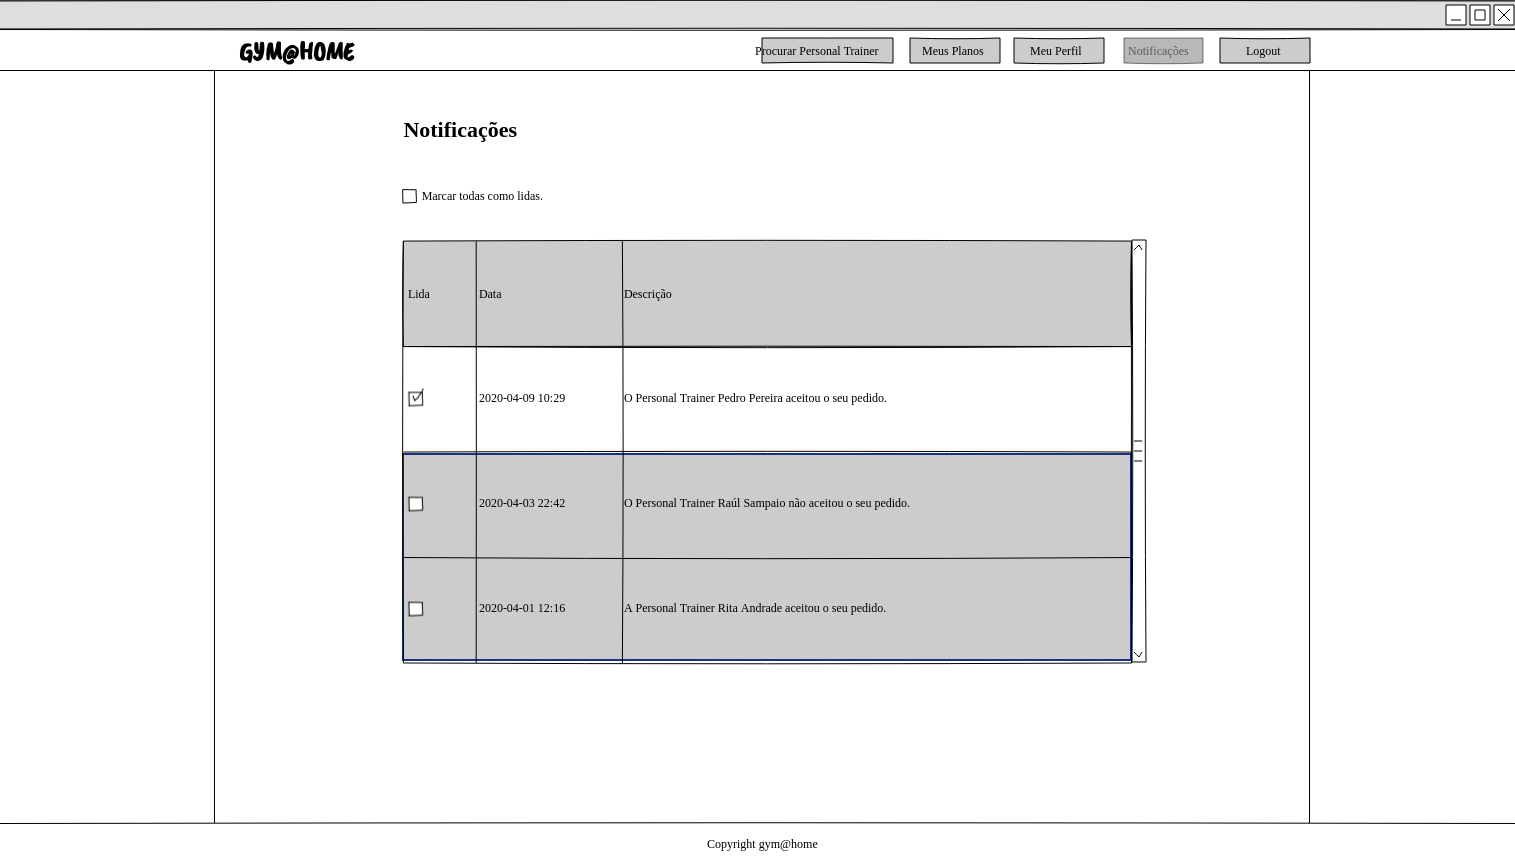
\includegraphics[scale=0.25]{images/mockups/cliente_notificaes.png}
    \caption{Mockup Notificações Cliente.}
    \label{fig:mockupnotificacoescliente}
\end{figure}

\begin{figure}[H]
    \centering
    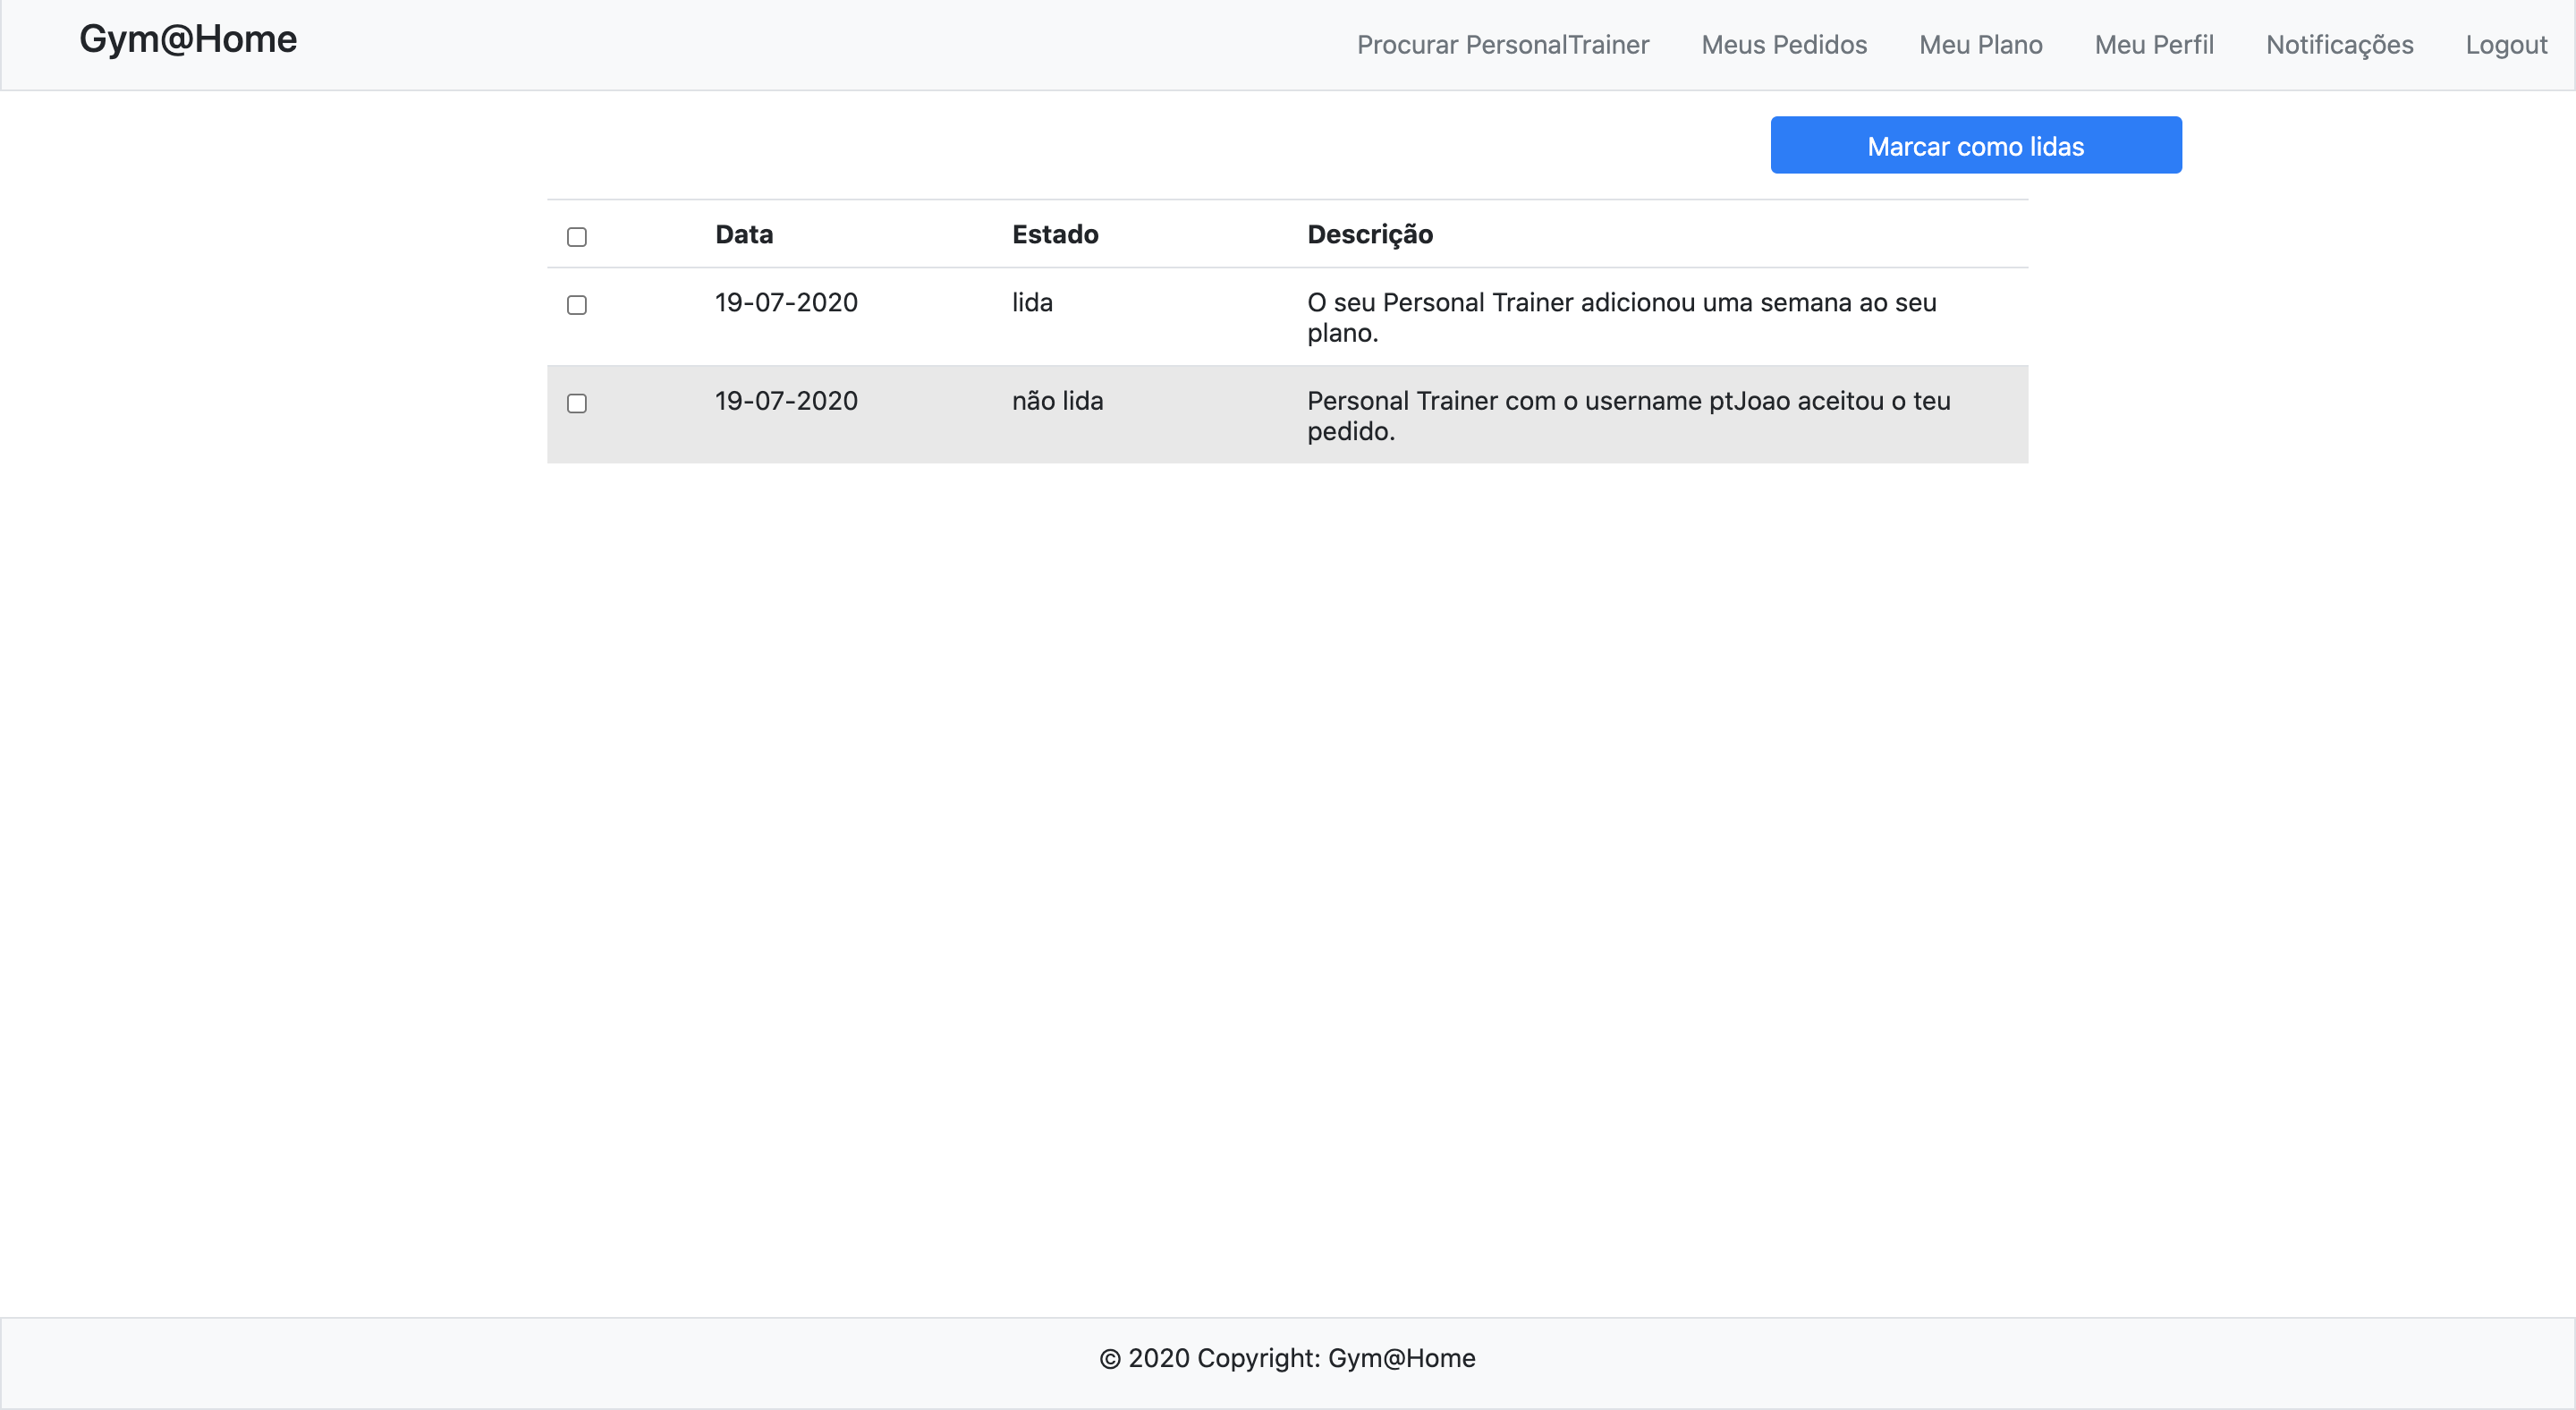
\includegraphics[scale=0.25]{images/interfaces/client_notifications.png}
    \caption{Interface Notificações Cliente.}
    \label{fig:interfacenotificacoescliente}
\end{figure}

\subsubsection{Princípios de usabilidade}
\begin{itemize}
    \item \textbf{Predictability}: quando se selecciona a checkbox para seleccionar todas as notificações para marcar como lidas, apenas selecciona as não lidas, para evitar que se envie o pedido de marcar como lida para o servidor desnecessariamente para notificações que já estão lidas
    \item \textbf{Synthesizability}: após marcar como lidas, as notificações aparecem com uma cor de background diferente, permitindo ao utilizador perceber o efeito da sua acção.
    \item \textbf{Familiarity}: As notificações por ler tem uma cor diferente das notificações lidas, um padrão \textbf{comum}.

\end{itemize}

\subsubsection{Heurísticas de Normam}
\begin{itemize}
    \item \textbf{Visibility of System Status}: os utilizadores obtém informações sobre acções que acontecerem no sistema relacionadas com os mesmos, mas sem ter sido este a alterar o estado.
    \item \textbf{Error Prevetion}: quando selecciona o marcar todas como lidas, apenas selecciona as não lidas, para que não sejam mandados pedidos para o servidor desnecessariamente, tal como já tinha sido dito no princípio de \textbf{Predictability}.
\end{itemize}

%--------------------------------------------------------------------------%

\section{Interfaces Clientes}
\label{sec:mockupsclients}

\subsection{Registar Cliente}
\label{subsec:registarcliente}

\subsubsection{Descrição}

\hspace{5mm} De forma a que o Cliente se registe na aplicação é necessário este inserir alguns dados obrigatórios, tais como o nome, username, email, etc..., bem como dados opcionais relacionados com dados biométricos. No entanto, importante referir que dos dados obrigatórios excepcionalmente a altura e peso são dados obrigatórios.

\begin{figure}[H]
    \centering
    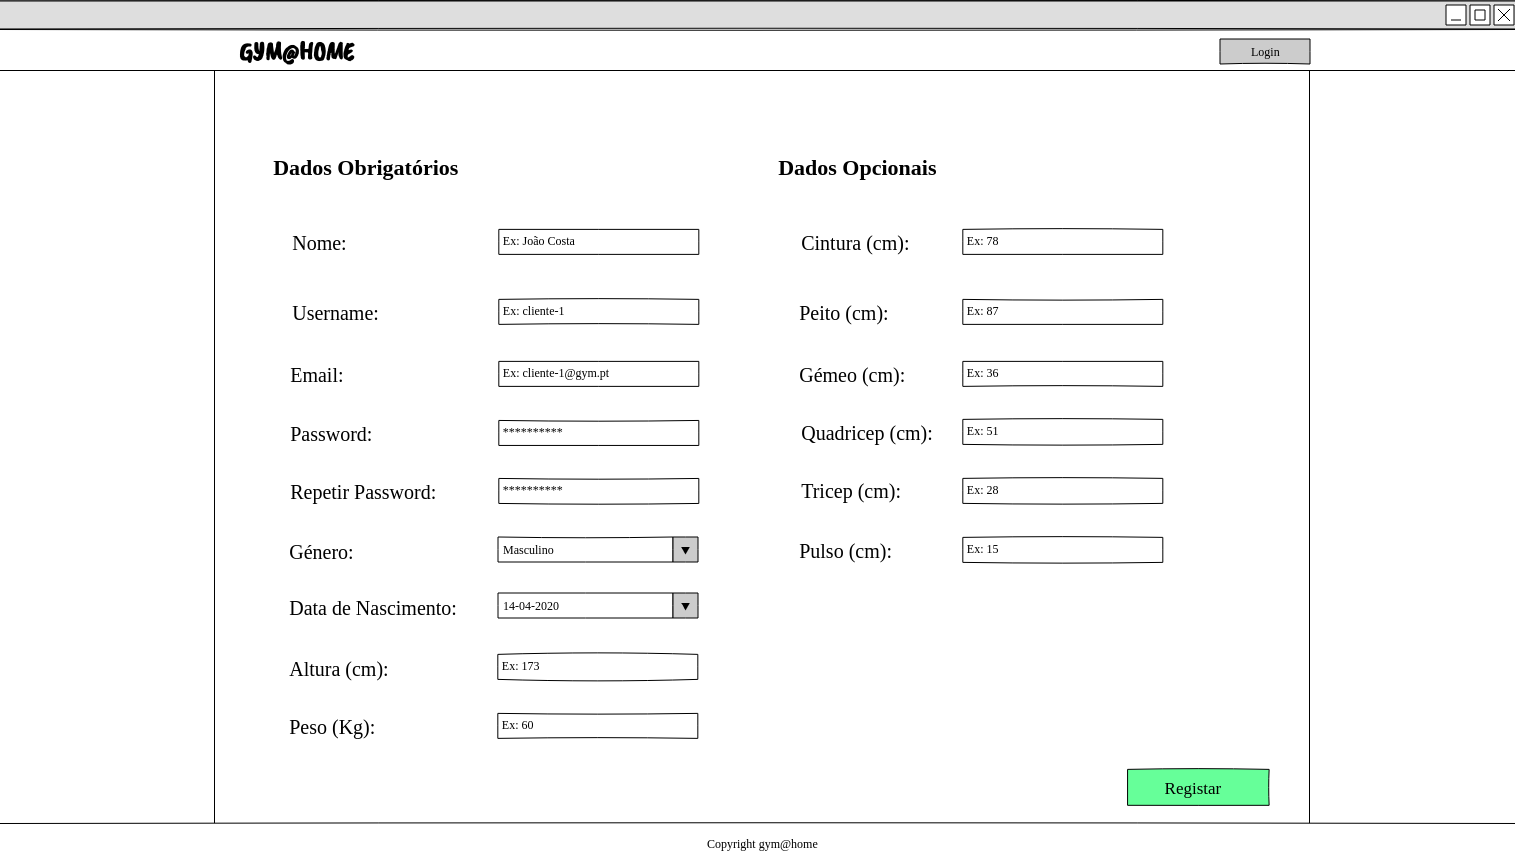
\includegraphics[scale=0.25]{images/mockups/cliente_registo_.png}
    \caption{Mockup Registar Cliente.}
    \label{fig:mockupregistarcliente}
\end{figure}

\begin{figure}[H]
    \centering
    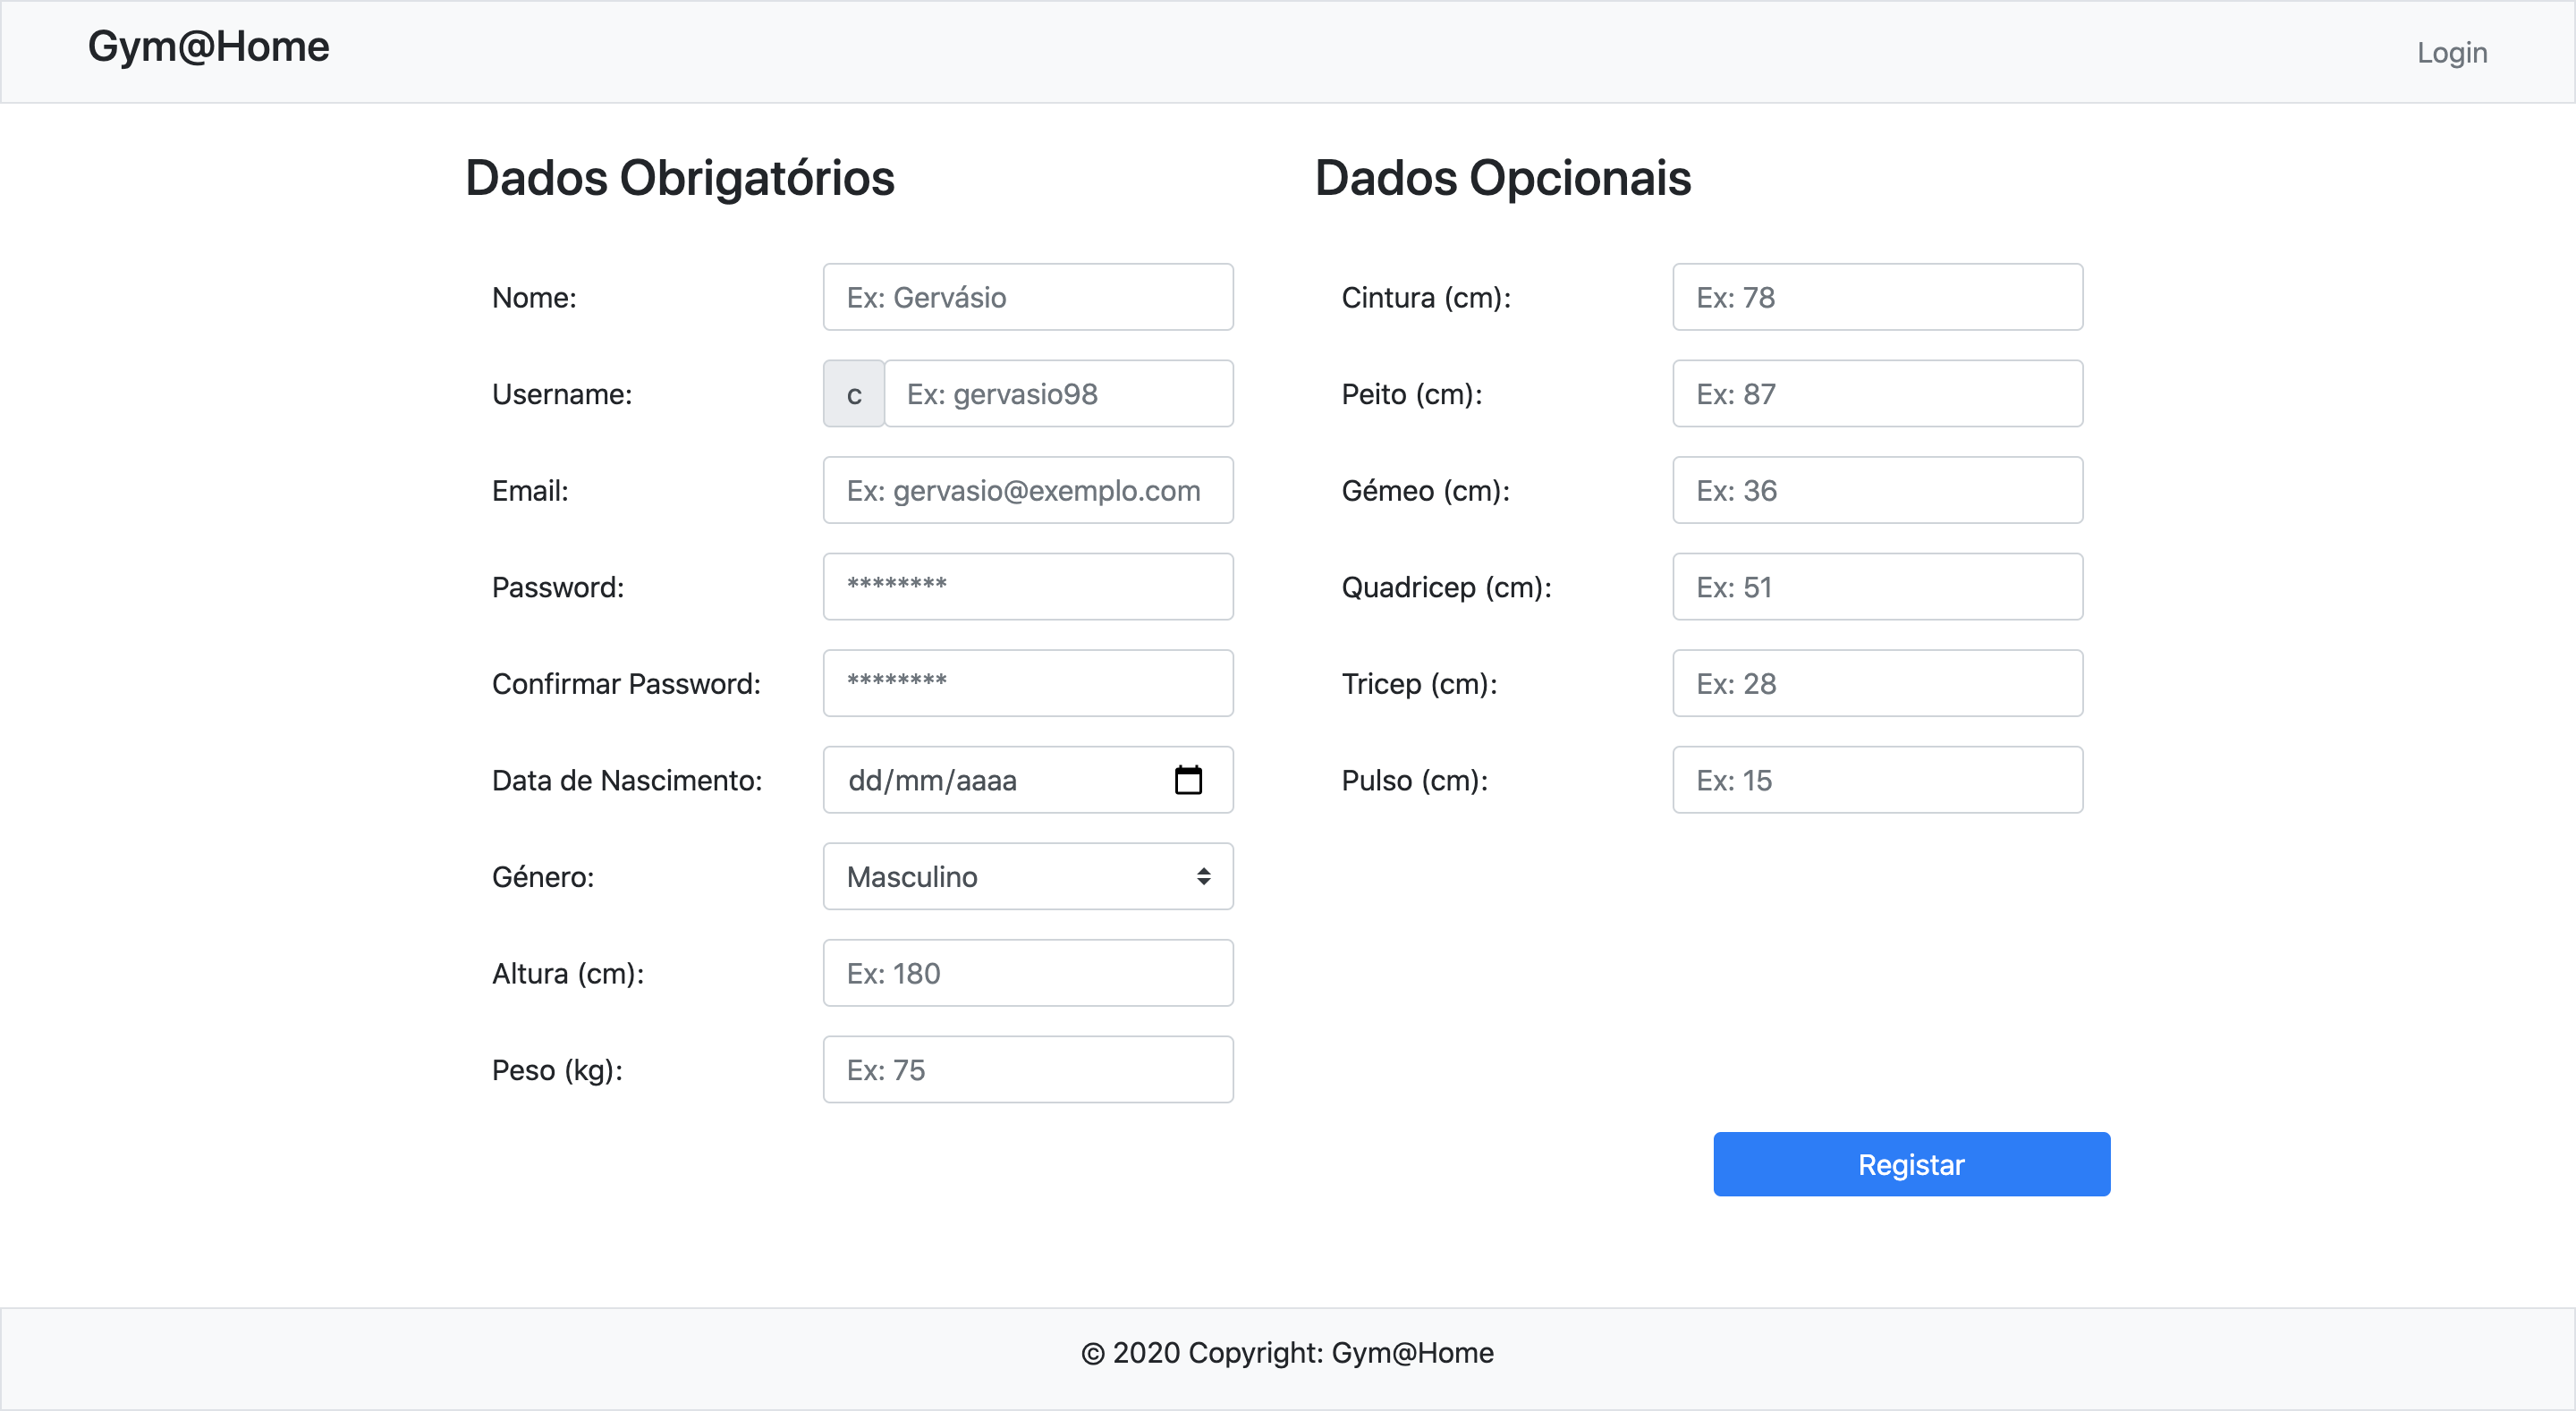
\includegraphics[scale=0.25]{images/interfaces/client_register.png}
    \caption{Interface Registar Cliente.}
    \label{fig:interfaceregistarcliente}
\end{figure}

\subsubsection{Princípios de Usabilidade}
\begin{itemize}
    \item \textbf{Familiarity}: Colocar a "Data de Nascimento" é feito através de um calendário, pelo que o Cliente como ser humano está mais familiarizado a utilizar.
    
\end{itemize}

\subsubsection{Heurísticas de Normam}
\begin{itemize}
    \item \textbf{Error prevention}: Todos os inputs numéricos aceitam apenas números, o "Género" apenas permite os valores do dropdown, a "Data de Nascimento" apenas permite datas seleccionadas pelo calendário e o "Email" apenas aceita um email (tem de conter o @).
    \textbf{Flexibility and efficiency of use}: visto que após ser feito o registo, faz-se o login automático, sendo mais \textbf{eficiente para o cliente}.
    
\end{itemize}

\subsection{Cliente consulta/edita o próprio perfil}
\label{subsec:perfilclientebycliente}

\subsubsection{Descrição}
\hspace{5mm} O mockup \textsc{Perfil do Cliente}, permite ao Cliente visualizar, bem como, editar o seu próprio perfil para manter as suas informações mais actualizadas possíveis. De forma a ficar mais consistente com o Registo de um Cliente na interface foram mantidas as duas colunas de dados, sendo que no cimo da página ficam os dados pessoais, de seguida os dados biométricos e a barra sobre o estado do IMC segundo os valores de referência da OMS.

\hspace{5mm} A submissão das alterações efectuadas ao perfil, basta alterar os dados que ele necessitar e carregar no botão "Salvar Alterações", este botão de forma a ficar mais visível na interface final foi colocado no cimo da página em vez de estar no fundo da mesma, pois em dispositivos mais pequenos o botão poderia ficar escondido.

\begin{figure}[H]
    \centering
    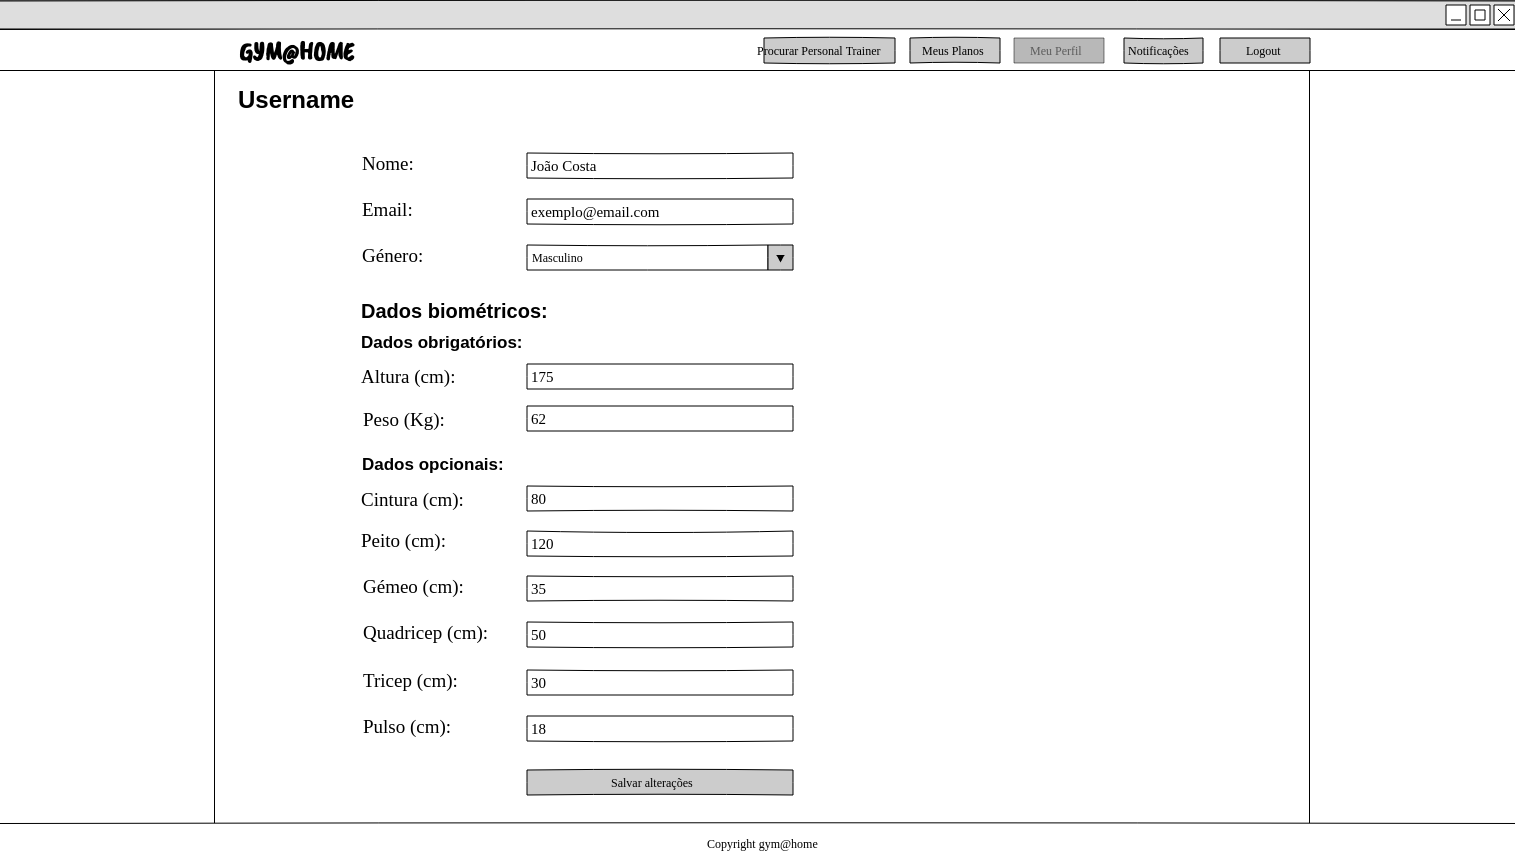
\includegraphics[scale=0.25]{images/mockups/pgina_meu_perfil_cliente.png}
    \caption{Mockup Perfil Cliente visto pelo próprio.}
    \label{fig:mockupperfilclientebycliente}
\end{figure}

\begin{figure}[H]
    \centering
    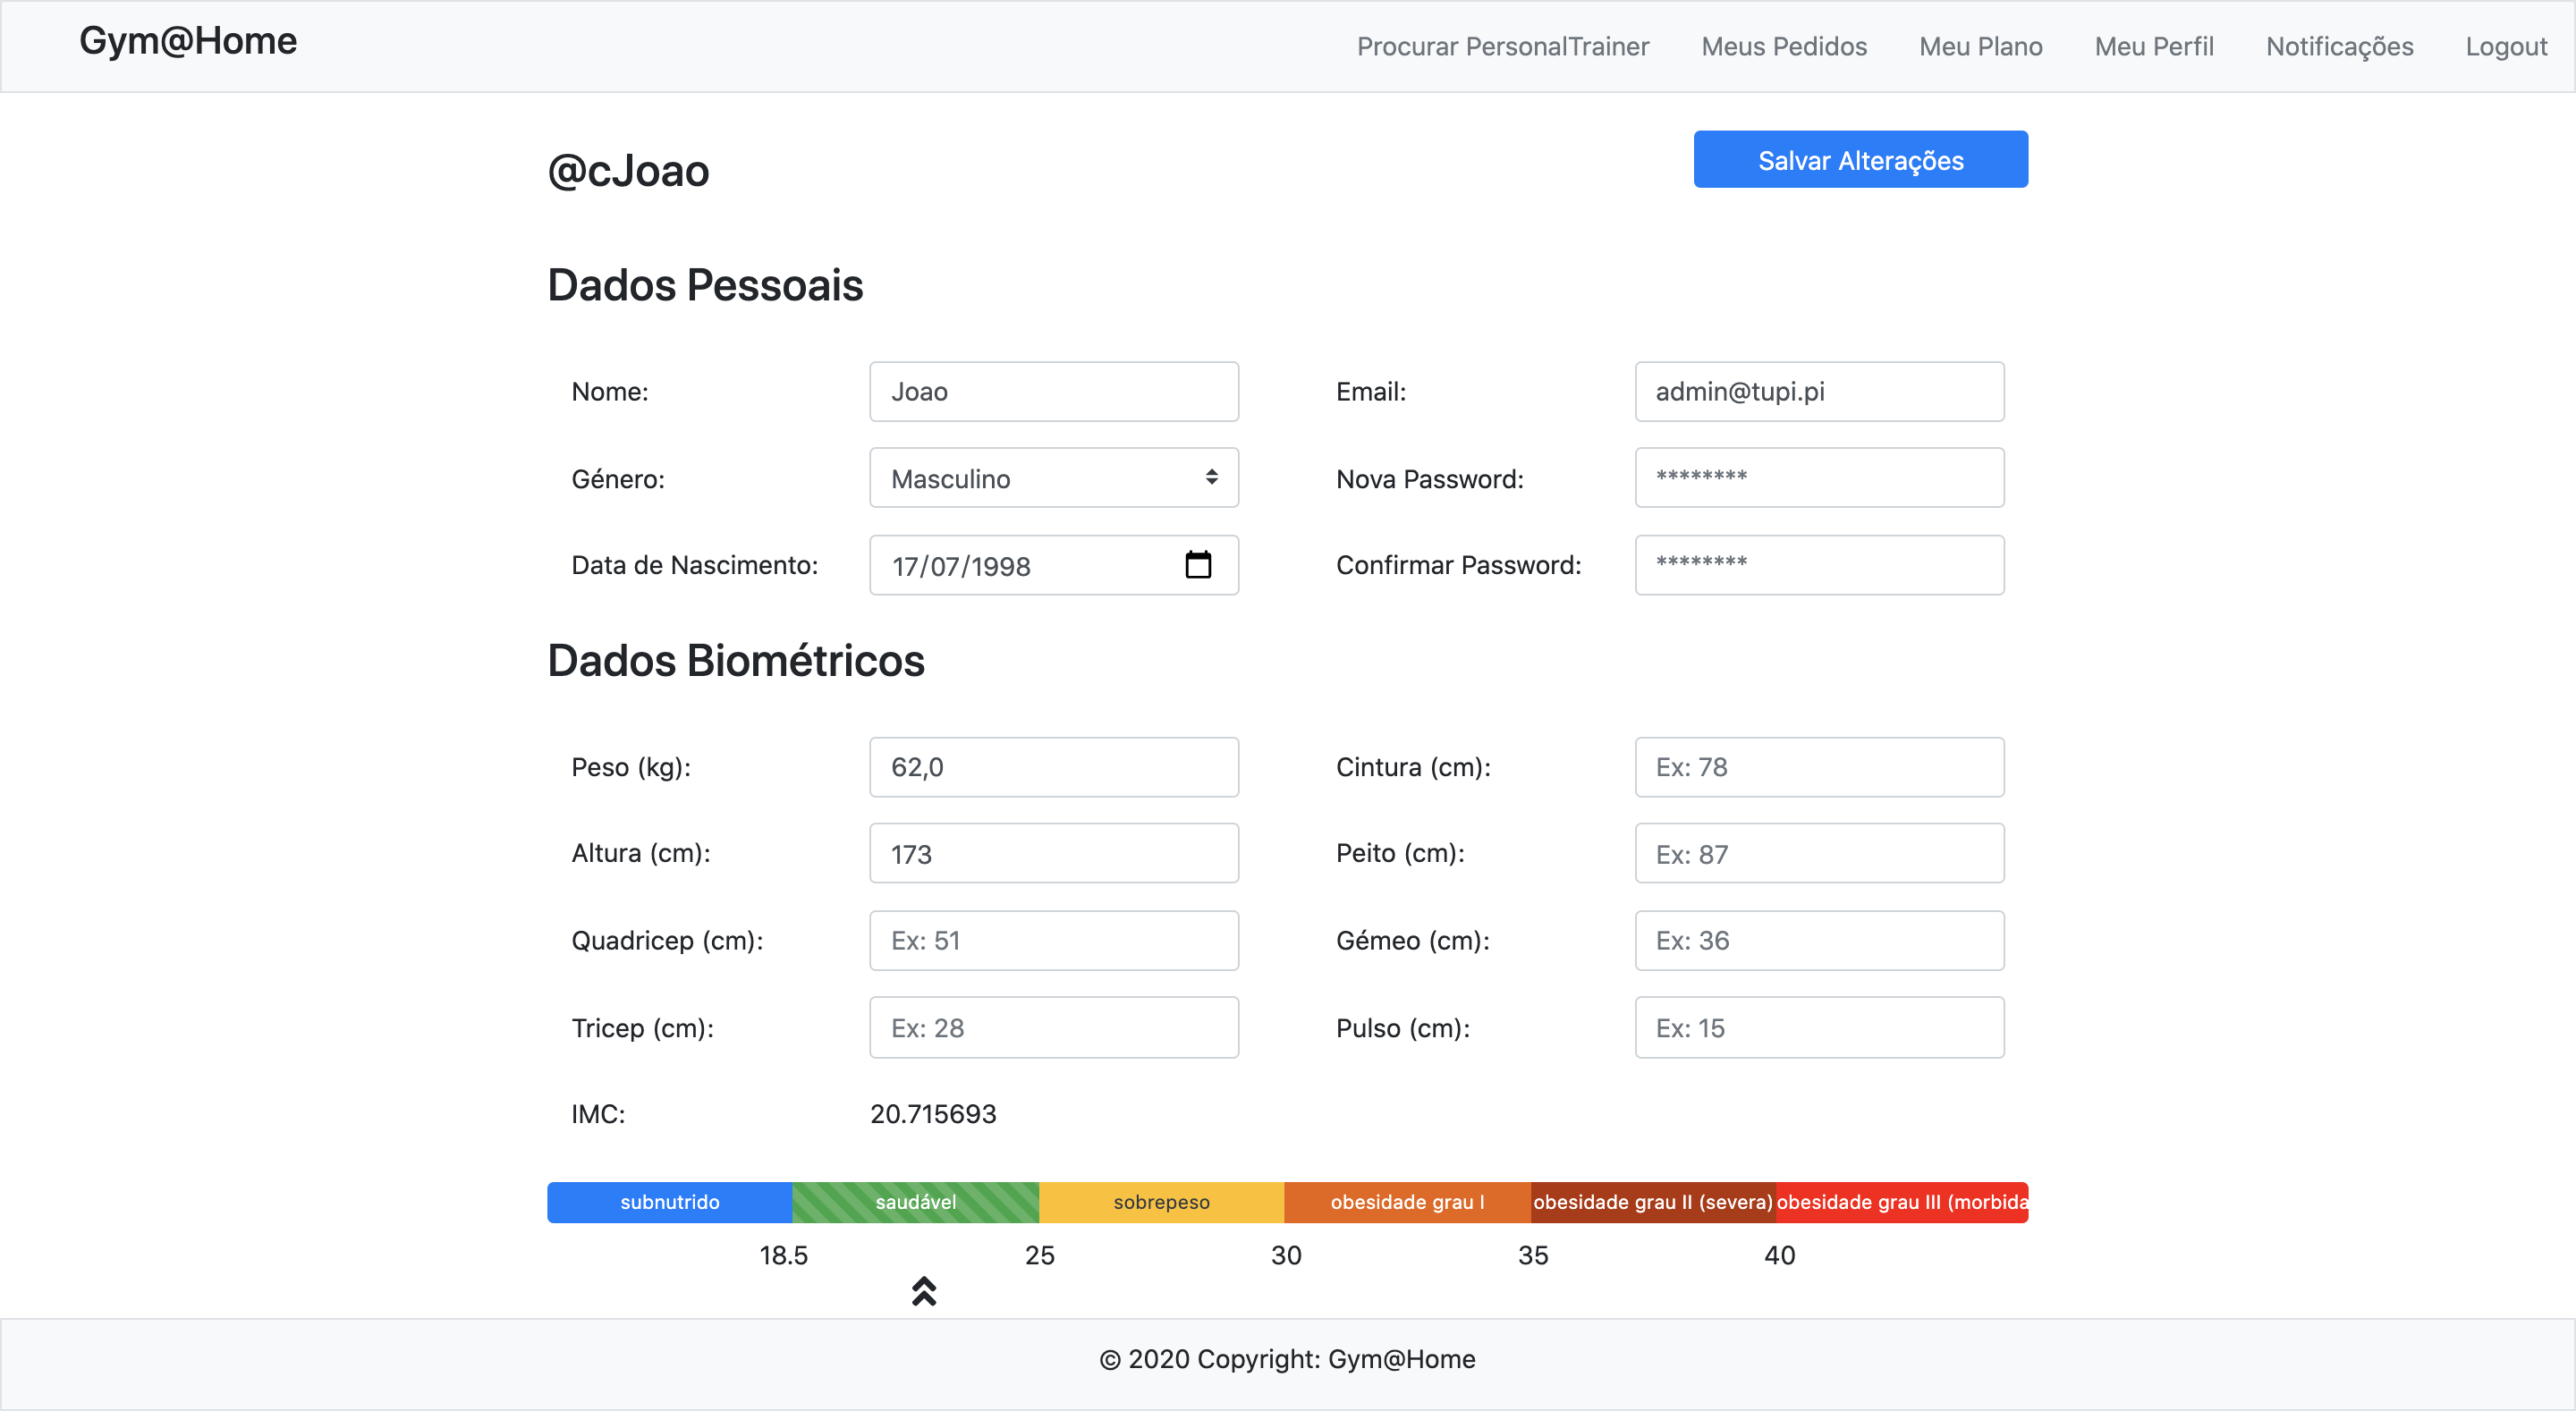
\includegraphics[scale=0.25]{images/interfaces/client_perfil.png}
    \caption{Interface Perfil Cliente visto pelo próprio.}
    \label{fig:interfaceperfilclientebycliente}
\end{figure}

\subsubsection{Princípios de usabilidade}
\begin{itemize}
   \item \textbf{Substitutivity}: Os inputs da interface onde o Cliente pode alterar os valores são também outputs. Sempre que o Cliente alterar dados estes são guardados na BD e novamente carregados para os outputs que o Cliente tinha utilizado como input.
    
    \item \textbf{Observability}: O botão "Salvar Alterações" está no cimo da página para o Cliente o conseguir observar mal carregue a página.
    
    \item \textbf{Familiarity}: Colocar a "Data de Nascimento" é feito através de um calendário, pelo que o Cliente como ser humano está mais familiarizado a utilizar.
    
\end{itemize}

\subsubsection{Heurísticas de Normam}
\begin{itemize}
    \item \textbf{Error prevention}: Todos os inputs numéricos aceitam apenas números, o "Género" apenas permite os valores do dropdown, a "Data de Nascimento" apenas permite datas seleccionadas pelo calendário e o "Email" apenas aceita um email (tem de conter o @).
    \item \textbf{Flexibility and efficiency of use}: tal como diz respeito ao principio \textbf{Substitutivity}, usar o mesmo componente quer para visualizar, quer para editar o perfil, torna a interface mais eficiente para o PT.
\end{itemize}

\subsection{Cliente consultar o perfil do PT}
\label{subsec:perfilptbycliente}

\subsubsection{Descrição}
\hspace{5mm} De forma a que o Cliente tenha uma visão mais detalhada do PT antes de realizar um pedido de Plano são mostradas algumas estatísticas do mesmo. De forma a que o Cliente disponha da informação do PT sem mudar de página este é ilustrado num pop-up, desta forma os filtros aplicados no refinamento dos PTs a observar são mantidos porque não é feito reload à página de "Procurar Personal Trainer".

\begin{figure}[H]
    \centering
    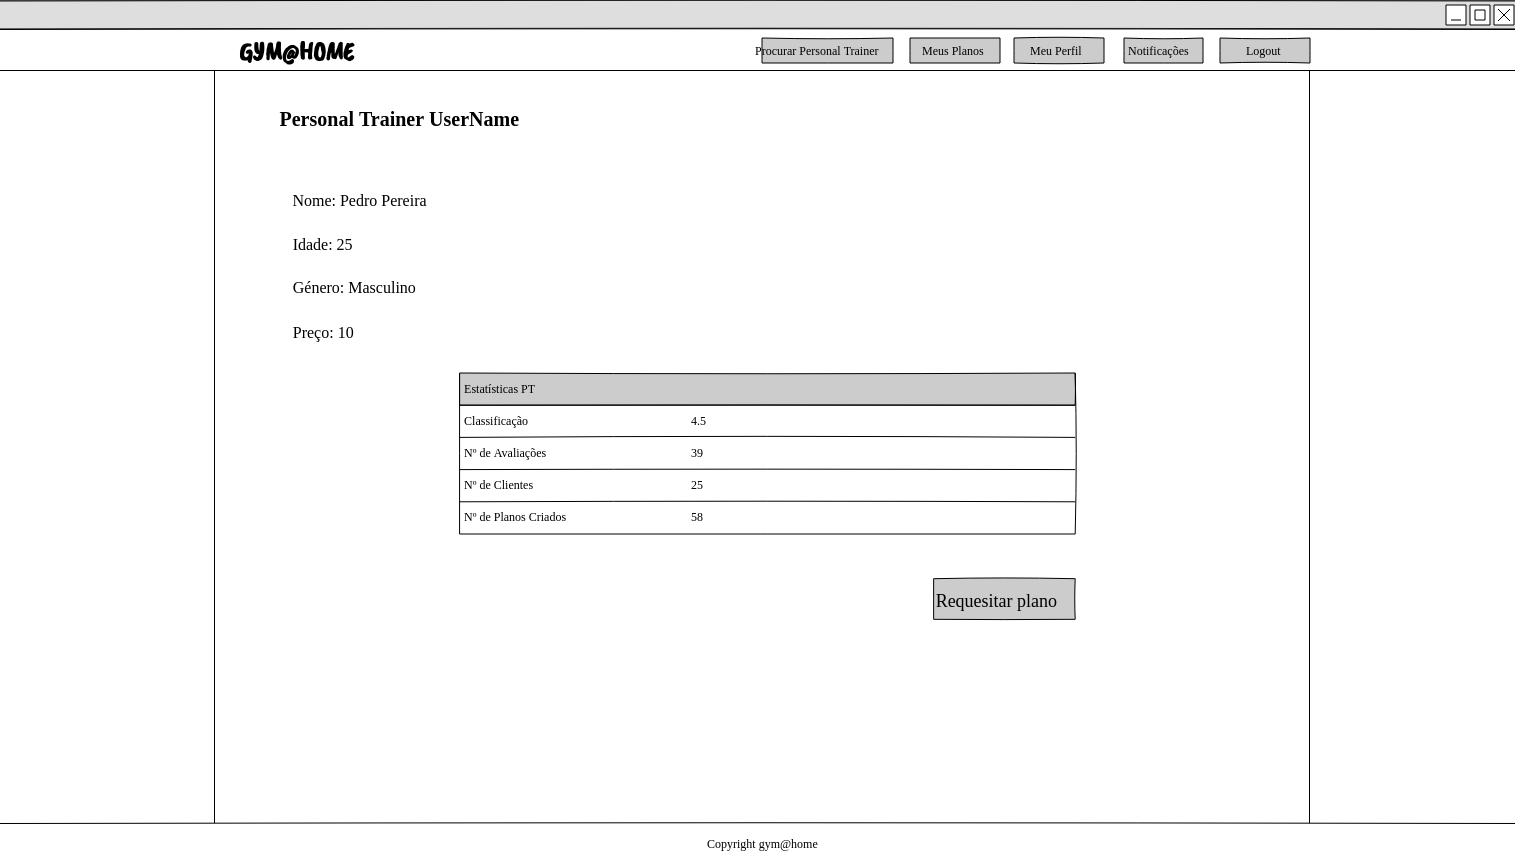
\includegraphics[scale=0.25]{images/mockups/cliente_perfil_personal_trainer.png}
    \caption{Mockup Perfil PT visto pelo Cliente.}
    \label{fig:mockupperfilptbycliente}
\end{figure}

\begin{figure}[H]
    \centering
    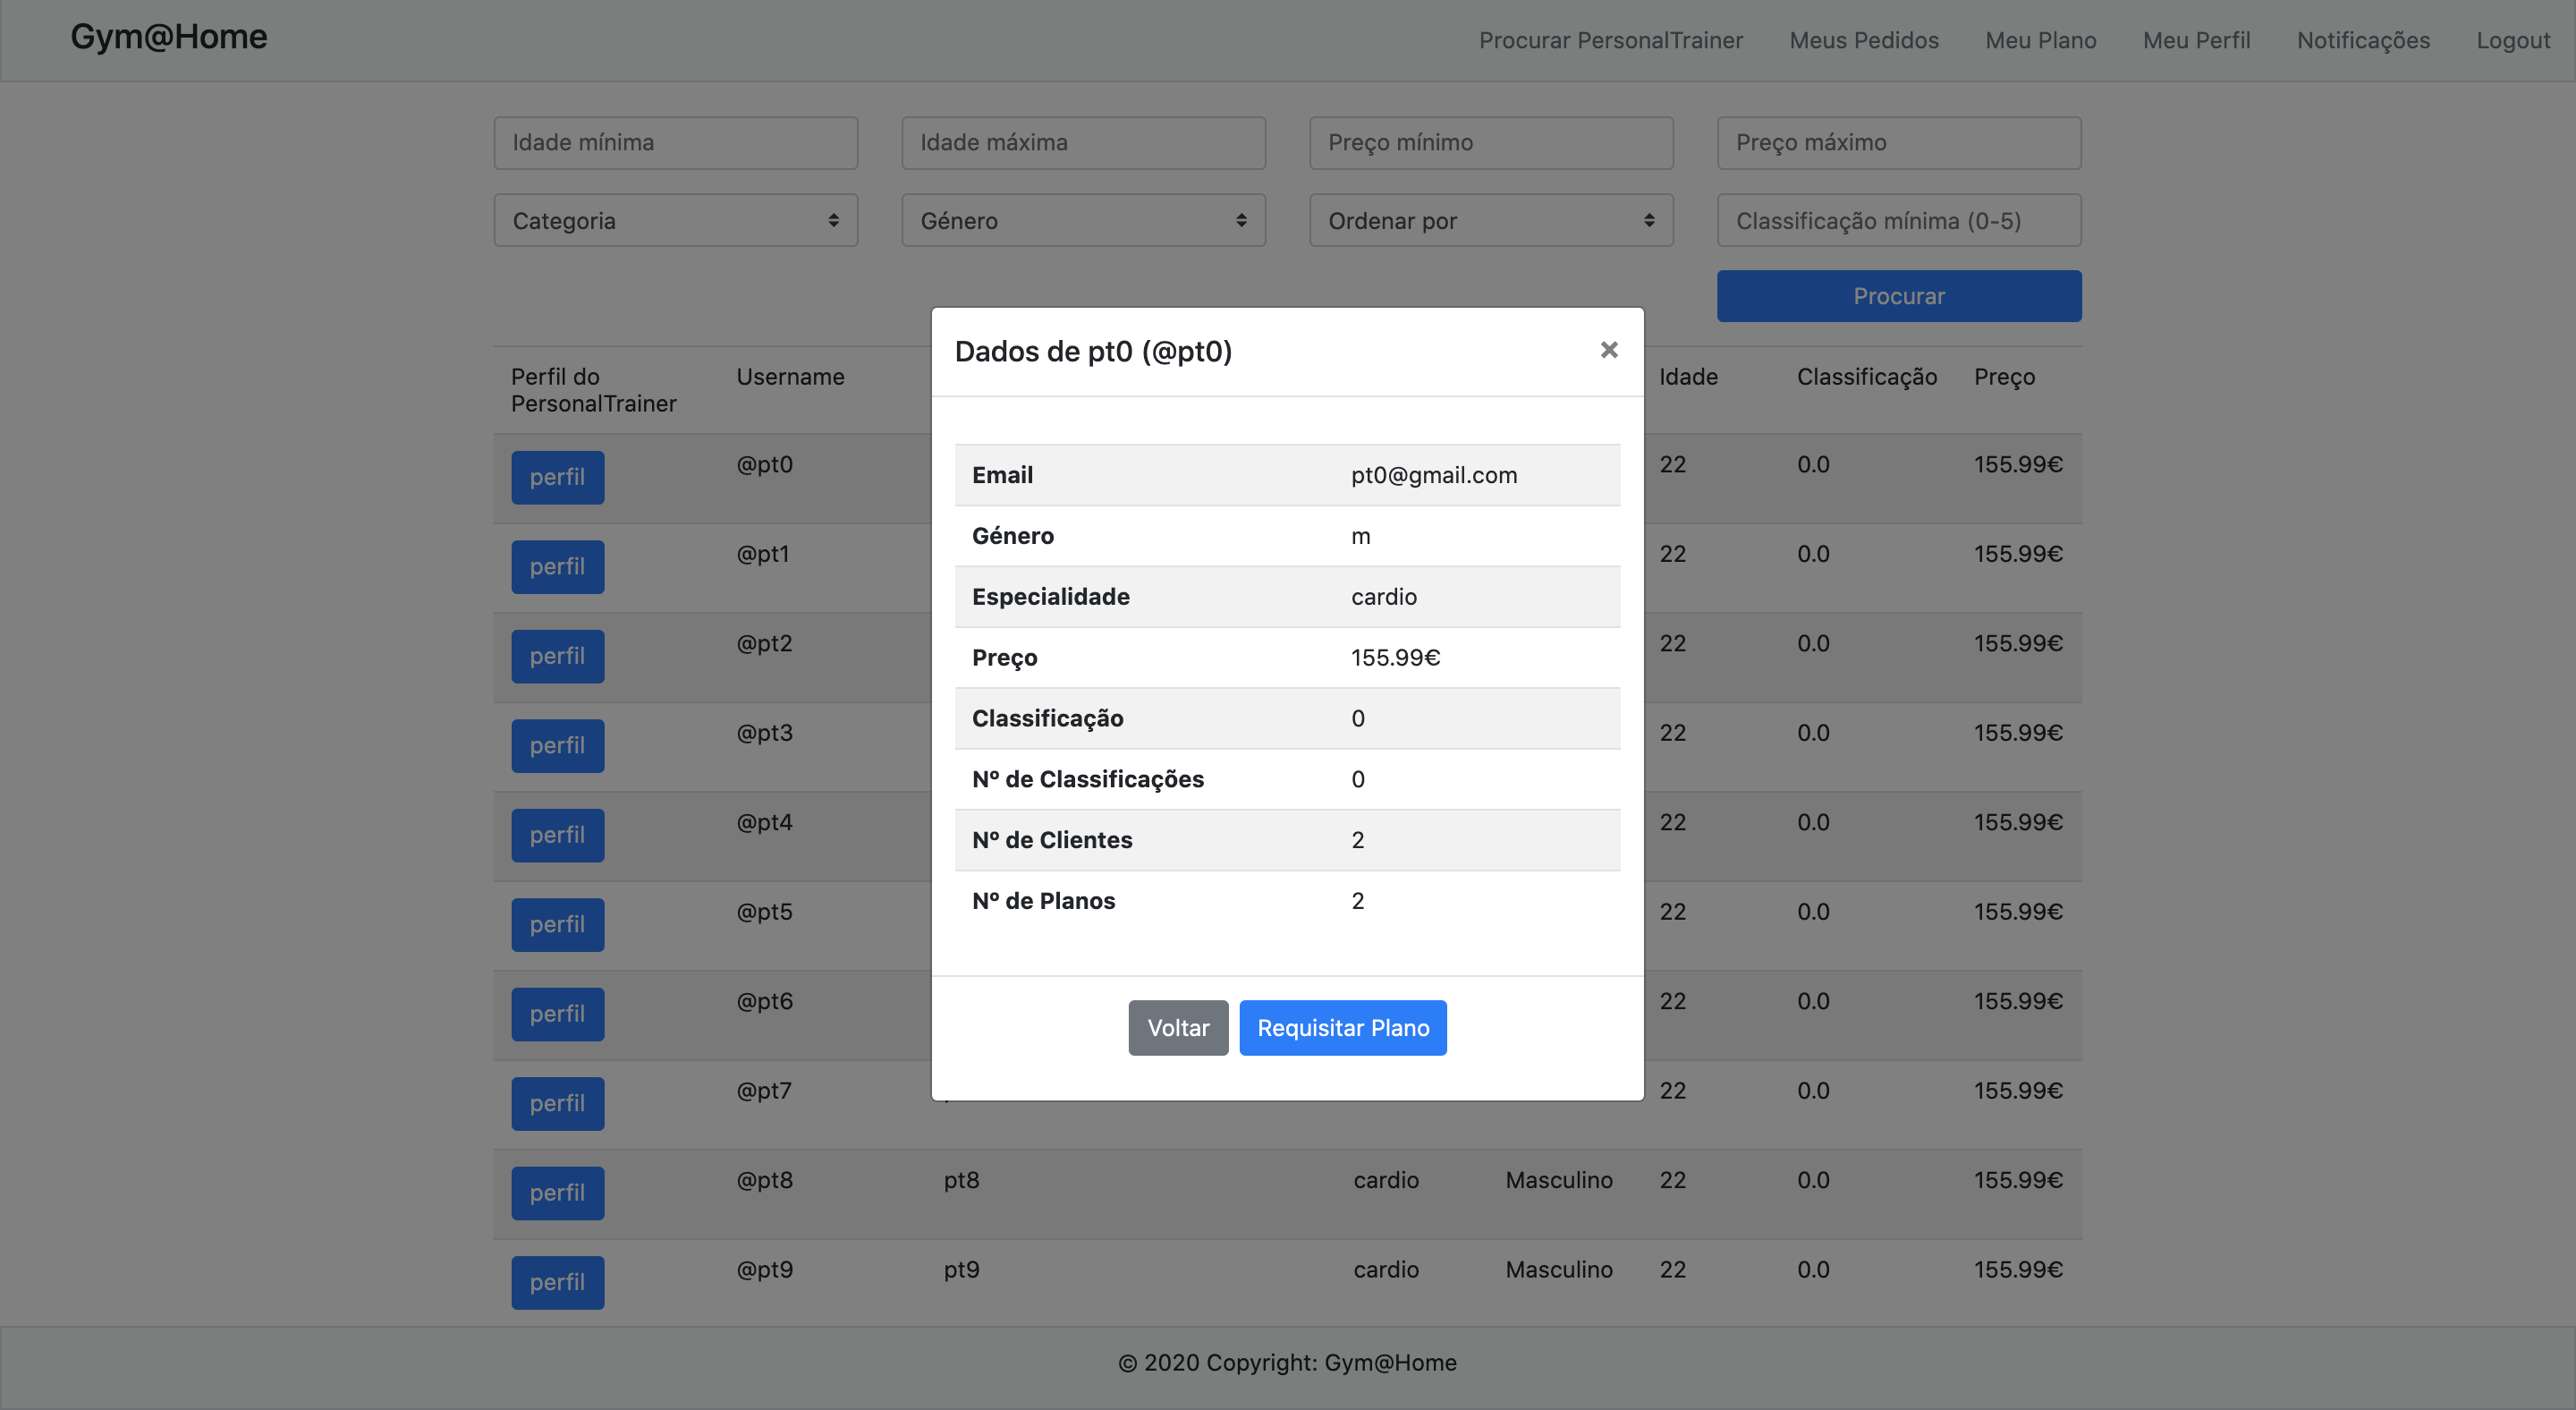
\includegraphics[scale=0.25]{images/interfaces/client_perfil_pt.png}
    \caption{Interface Perfil PT visto pelo Cliente.}
    \label{fig:interfaceperfilptbycliente}
\end{figure}

\subsubsection{Princípios de usabilidade}
\begin{itemize}
    \item \textbf{Generability} e \textbf{Consistency}: na medida em que a estrutura de apresentação deste pop-up com a informação do perfil torna-se semelhante para ambos os utilizadores quando desejam consultar a informação da entidade oposta.
\end{itemize}

\subsubsection{Heurísticas de Normam}
\begin{itemize}
    \item \textbf{Recognition rather than recall}: o cliente não necessita de lembrar-se/memorizar dos dados de perfil do PT, podendo consultá-los no momento em que precisa dos mesmos de forma eficiente.
    \item \textbf{Flexibility and efficiency of use}: o botão "perfil", que mostra as informações do PT torna esse processo de consulta mais \textbf{eficiente}, como uma espécie de atalho.
\end{itemize}

\subsection{Procurar Personal Trainer}
\label{subsec:procurarpersonaltrainer}

\subsubsection{Descrição}
\hspace{5mm} Nesta mockup são ilustrados todos os PTs disponíveis, aqui o Cliente pode aplicar filtros para uma pesquisa mais refinada por PTs que possam ser do seu interesse. Devido ao tamanho dos filtros e respectivo conteúdo estes não cabiam numa única linha tal como na mockup pelo que na interface final estes aparecem em duas linhas, ficando assim mais legíveis para o Cliente.

\hspace{5mm} Tal como foi mostrado no mockup anterior, cada linha, que corresponde a um PT contém um botão denominado "perfil" que apresenta um pop-up com as informações do perfil do PT, onde se encontram algumas informações adicionais.

\begin{figure}[H]
    \centering
    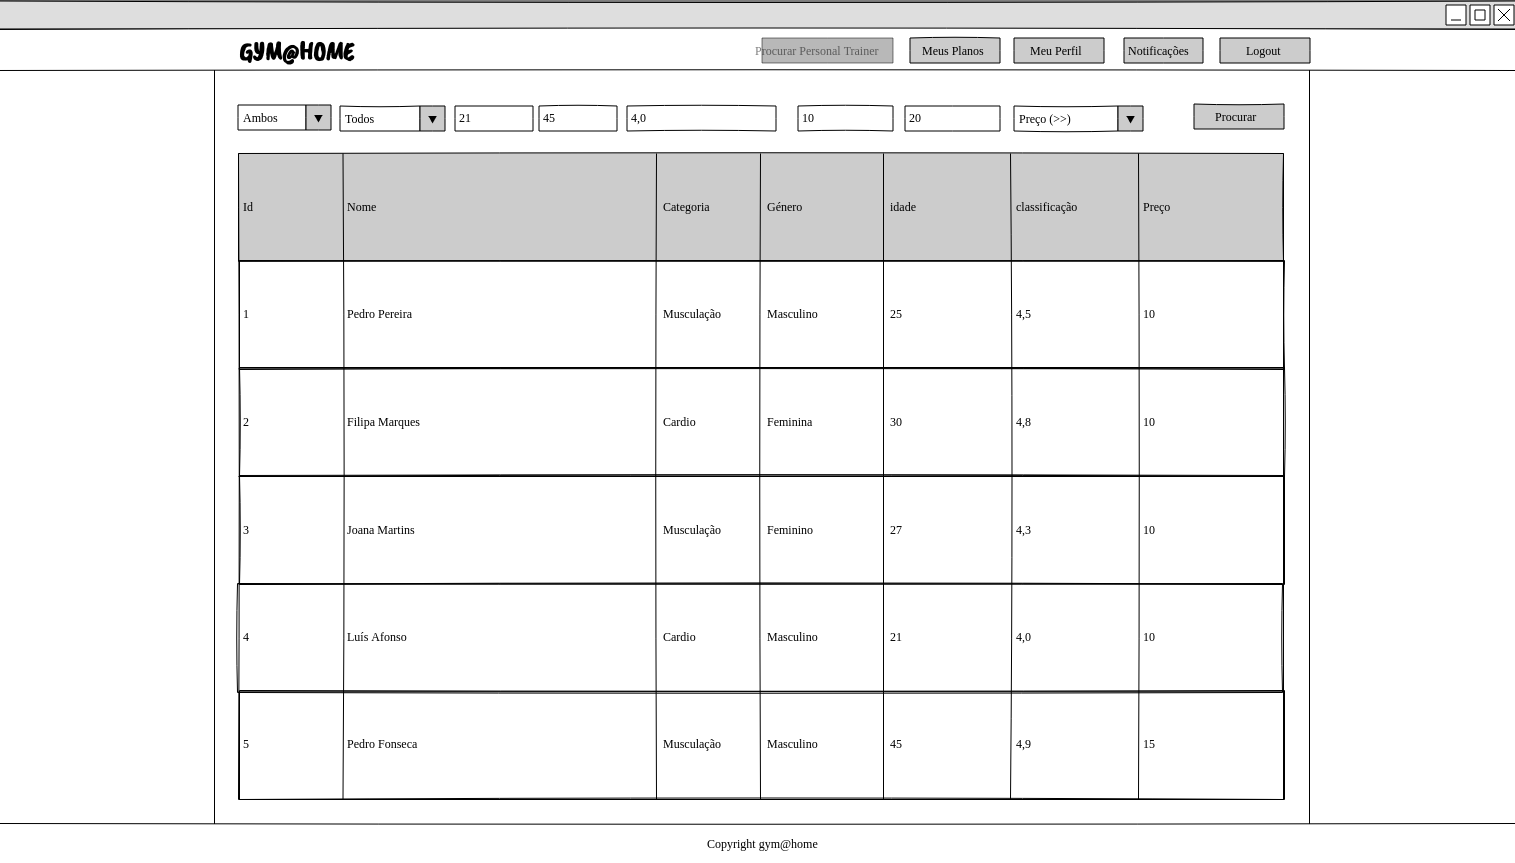
\includegraphics[scale=0.25]{images/mockups/procurar_com_filtros_tabela_preenchida.png}
    \caption{Mockup Procurar Personal Trainer.}
    \label{fig:mockupprocurarpersonaltrainer}
\end{figure}

\begin{figure}[H]
    \centering
    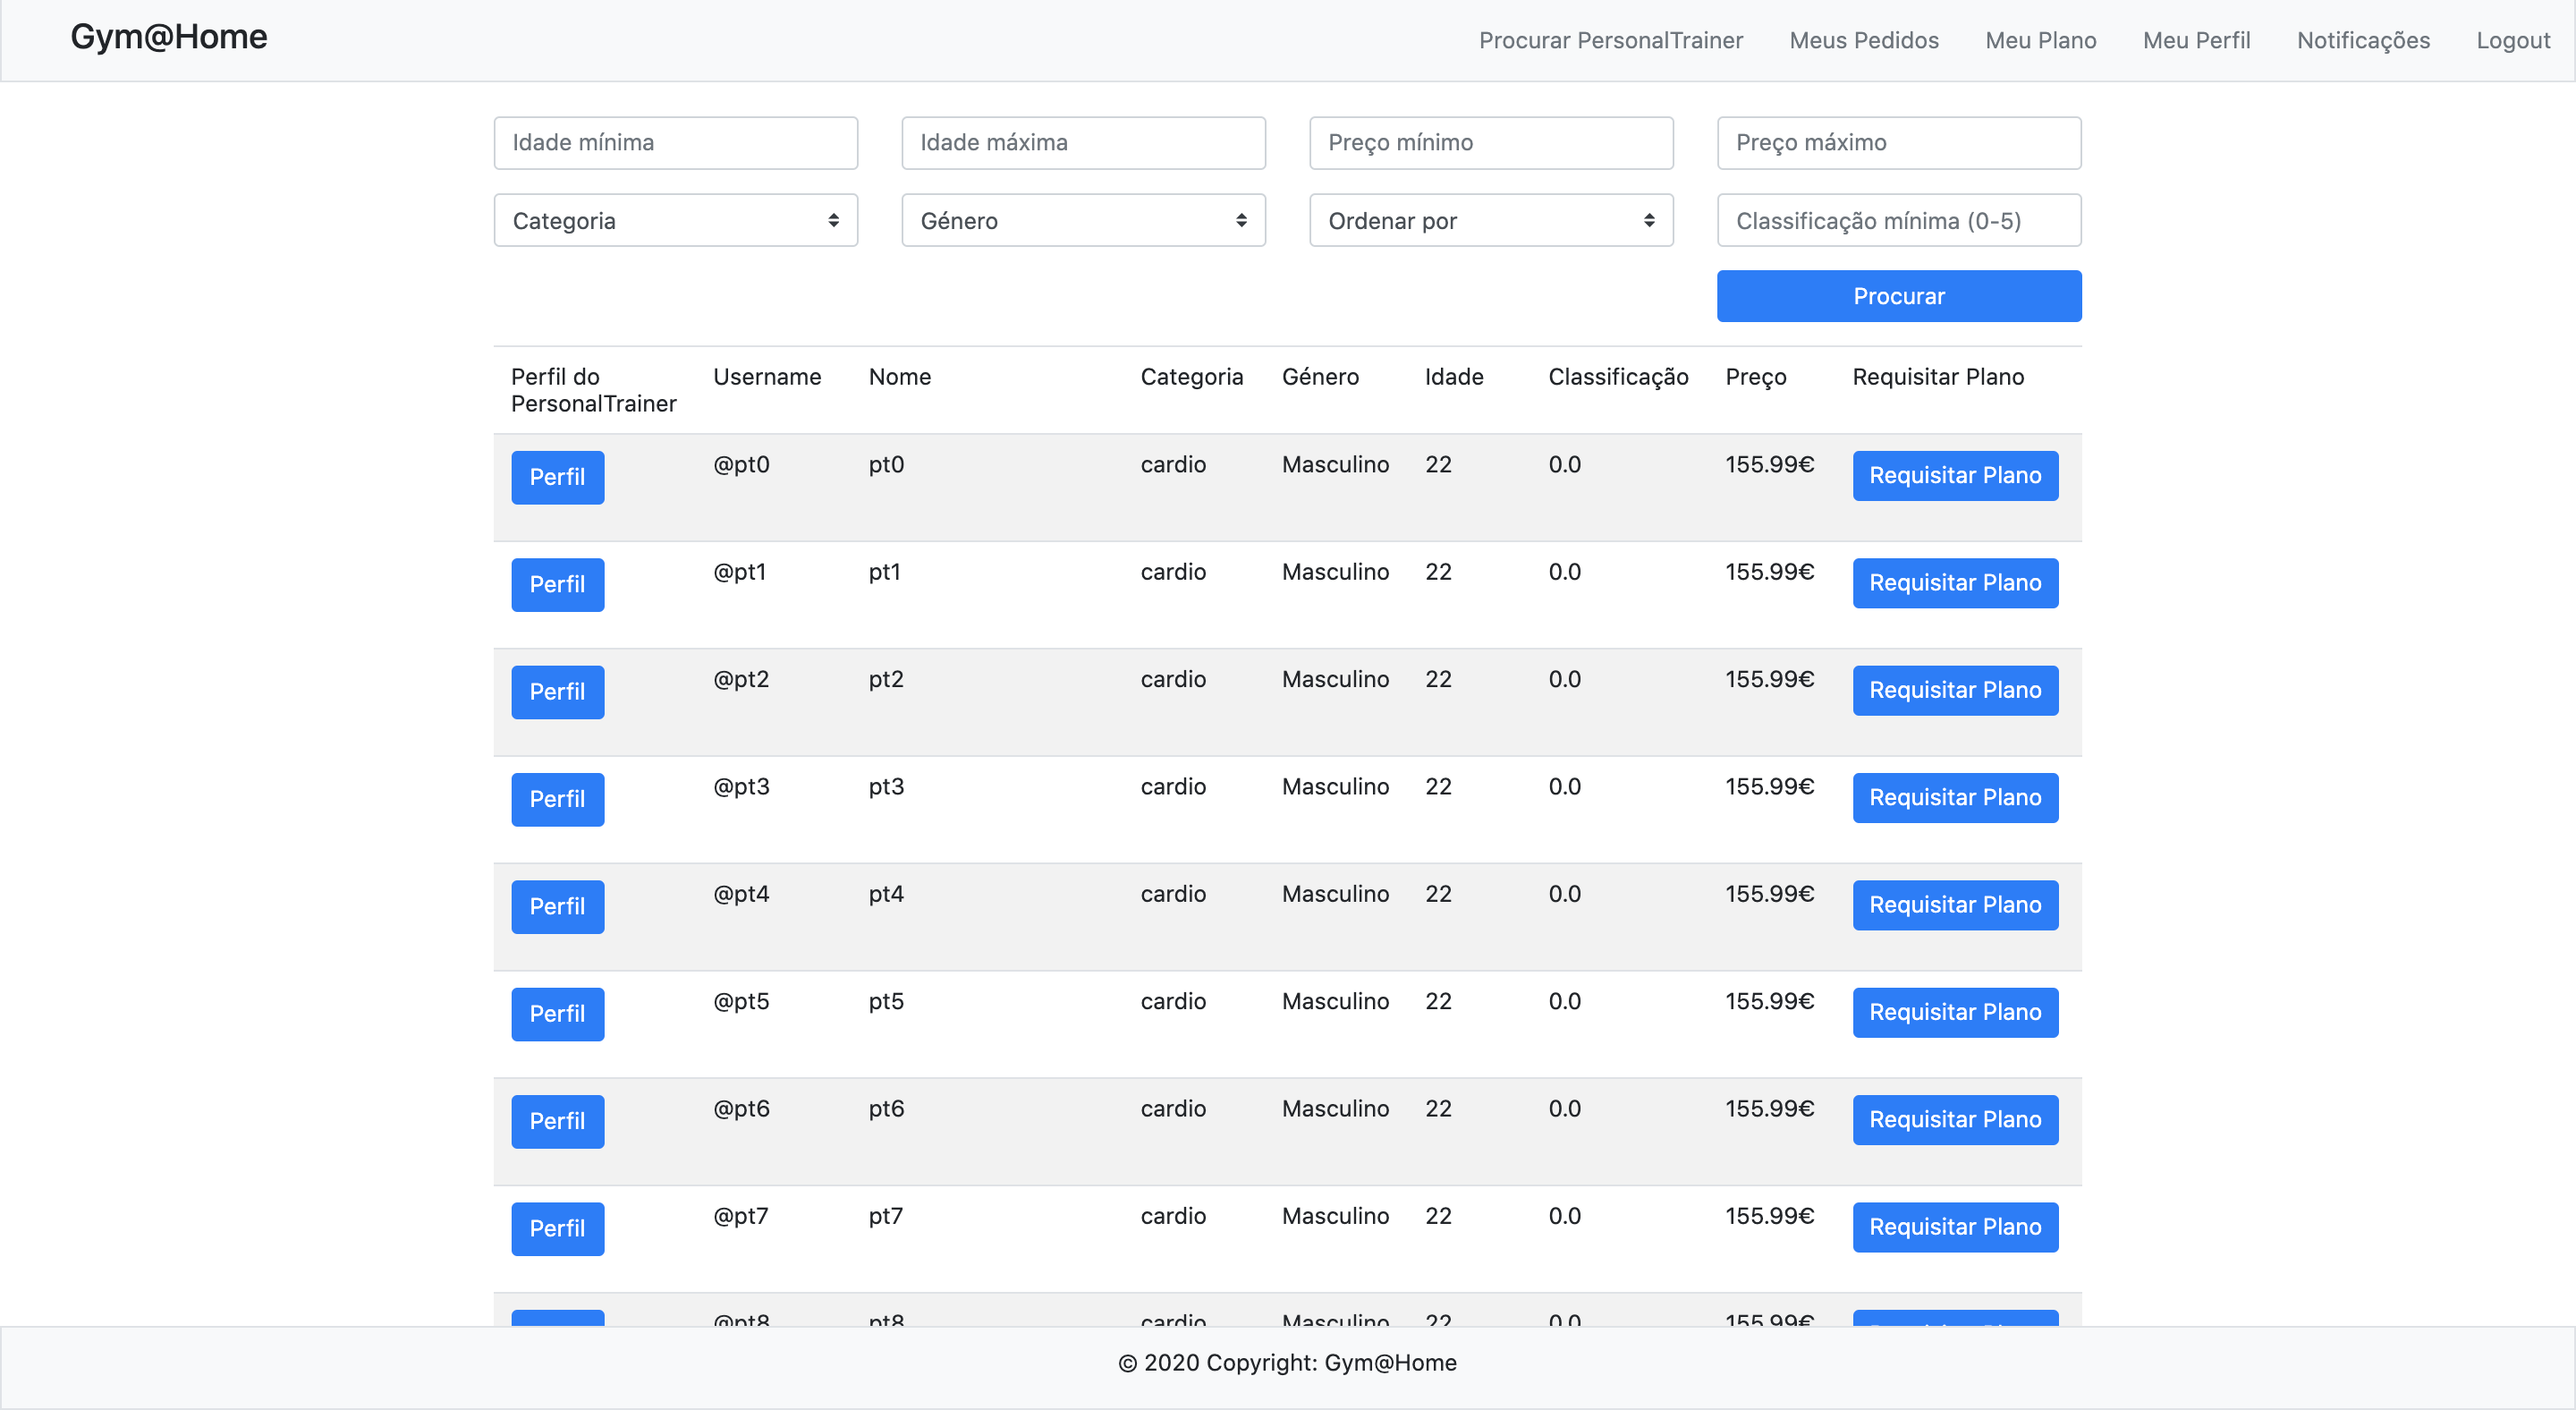
\includegraphics[scale=0.25]{images/interfaces/client_procurar_pt.png}
    \caption{Interface Procurar Personal Trainer.}
    \label{fig:interfaceprocurarpersonaltrainer}
\end{figure}

\subsubsection{Princípios de usabilidade}
\begin{itemize}
    \item \textbf{Synthesizability}: nesta interface, existem duas situações deste princípio: inicialmente quando são listados todos os PTs, isto é, consegue perceber o efeito da sua acção, por outro lado, quando selecciona um PT e deseja requisitar um plano do mesmo, redirecciona-se para a página para esse efeito, e dessa forma, também consegue perceber o efeito da sua acção.
    \item \textbf{Familiarity}: a estrutura utilizada para a filtragem seguiu o padrão comum, que se pode encontrar em muitas aplicações web.
\end{itemize}

\subsubsection{Heurísticas de Normam}
\begin{itemize}
    \item \textbf{Error prevention}: Todos os inputs numéricos aceitam apenas números e o "Género", "Categoria" e "Ordenar Por" apenas permite os valores dos dropdowns.
    \item \textbf{Recognition rather than recall}: utilização de dropdowns nos filtros permite que o utilizador não tenha que memorizar as opções existentes.
    \item \textbf{Flexibility and efficiency of use}: o botão "perfil", que mostra as informações do PT torna esse processo de consulta mais \textbf{eficiente}, como uma espécie de atalho.
\end{itemize}

\subsection{Preencher Pedido}
\label{subsec:preencherpedido}

\subsubsection{Descrição}
\hspace{5mm} A requisição dum Plano, necessita do preenchimento de um formulário com alguns dados pelo Cliente. A mockup/protótipo e a interface final foi removida a opção de adicionar os dados biométricos opcionais do Cliente, sendo que todos os dados biométricos são enviados automaticamente ao PT.

\begin{figure}[H]
    \centering
    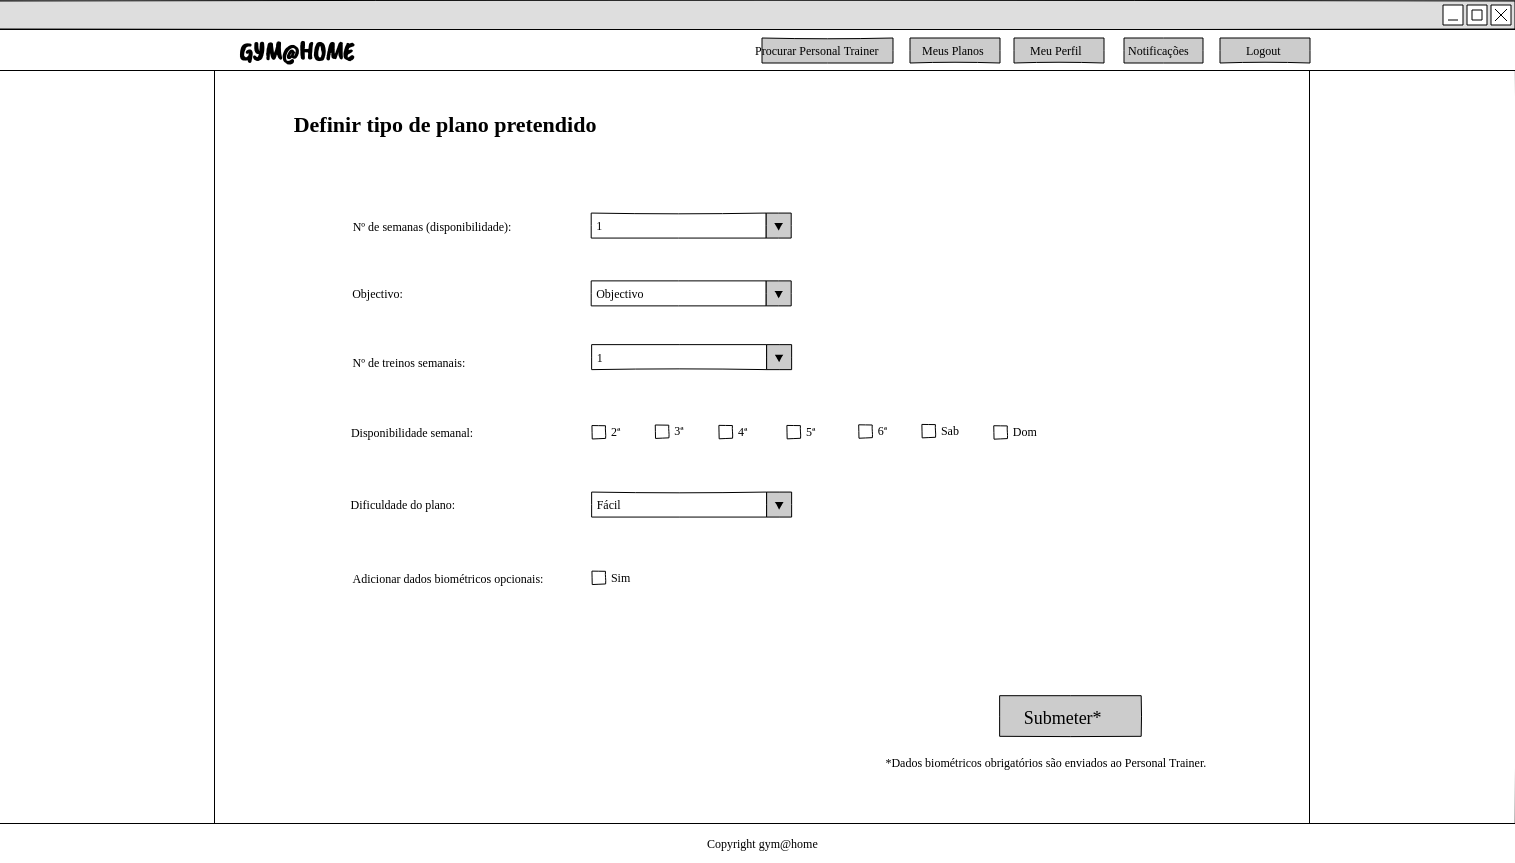
\includegraphics[scale=0.25]{images/mockups/cliente_formulrio.png}
    \caption{Mockup Preencher Pedido.}
    \label{fig:mockuppreencherpedido}
\end{figure}

\begin{figure}[H]
    \centering
    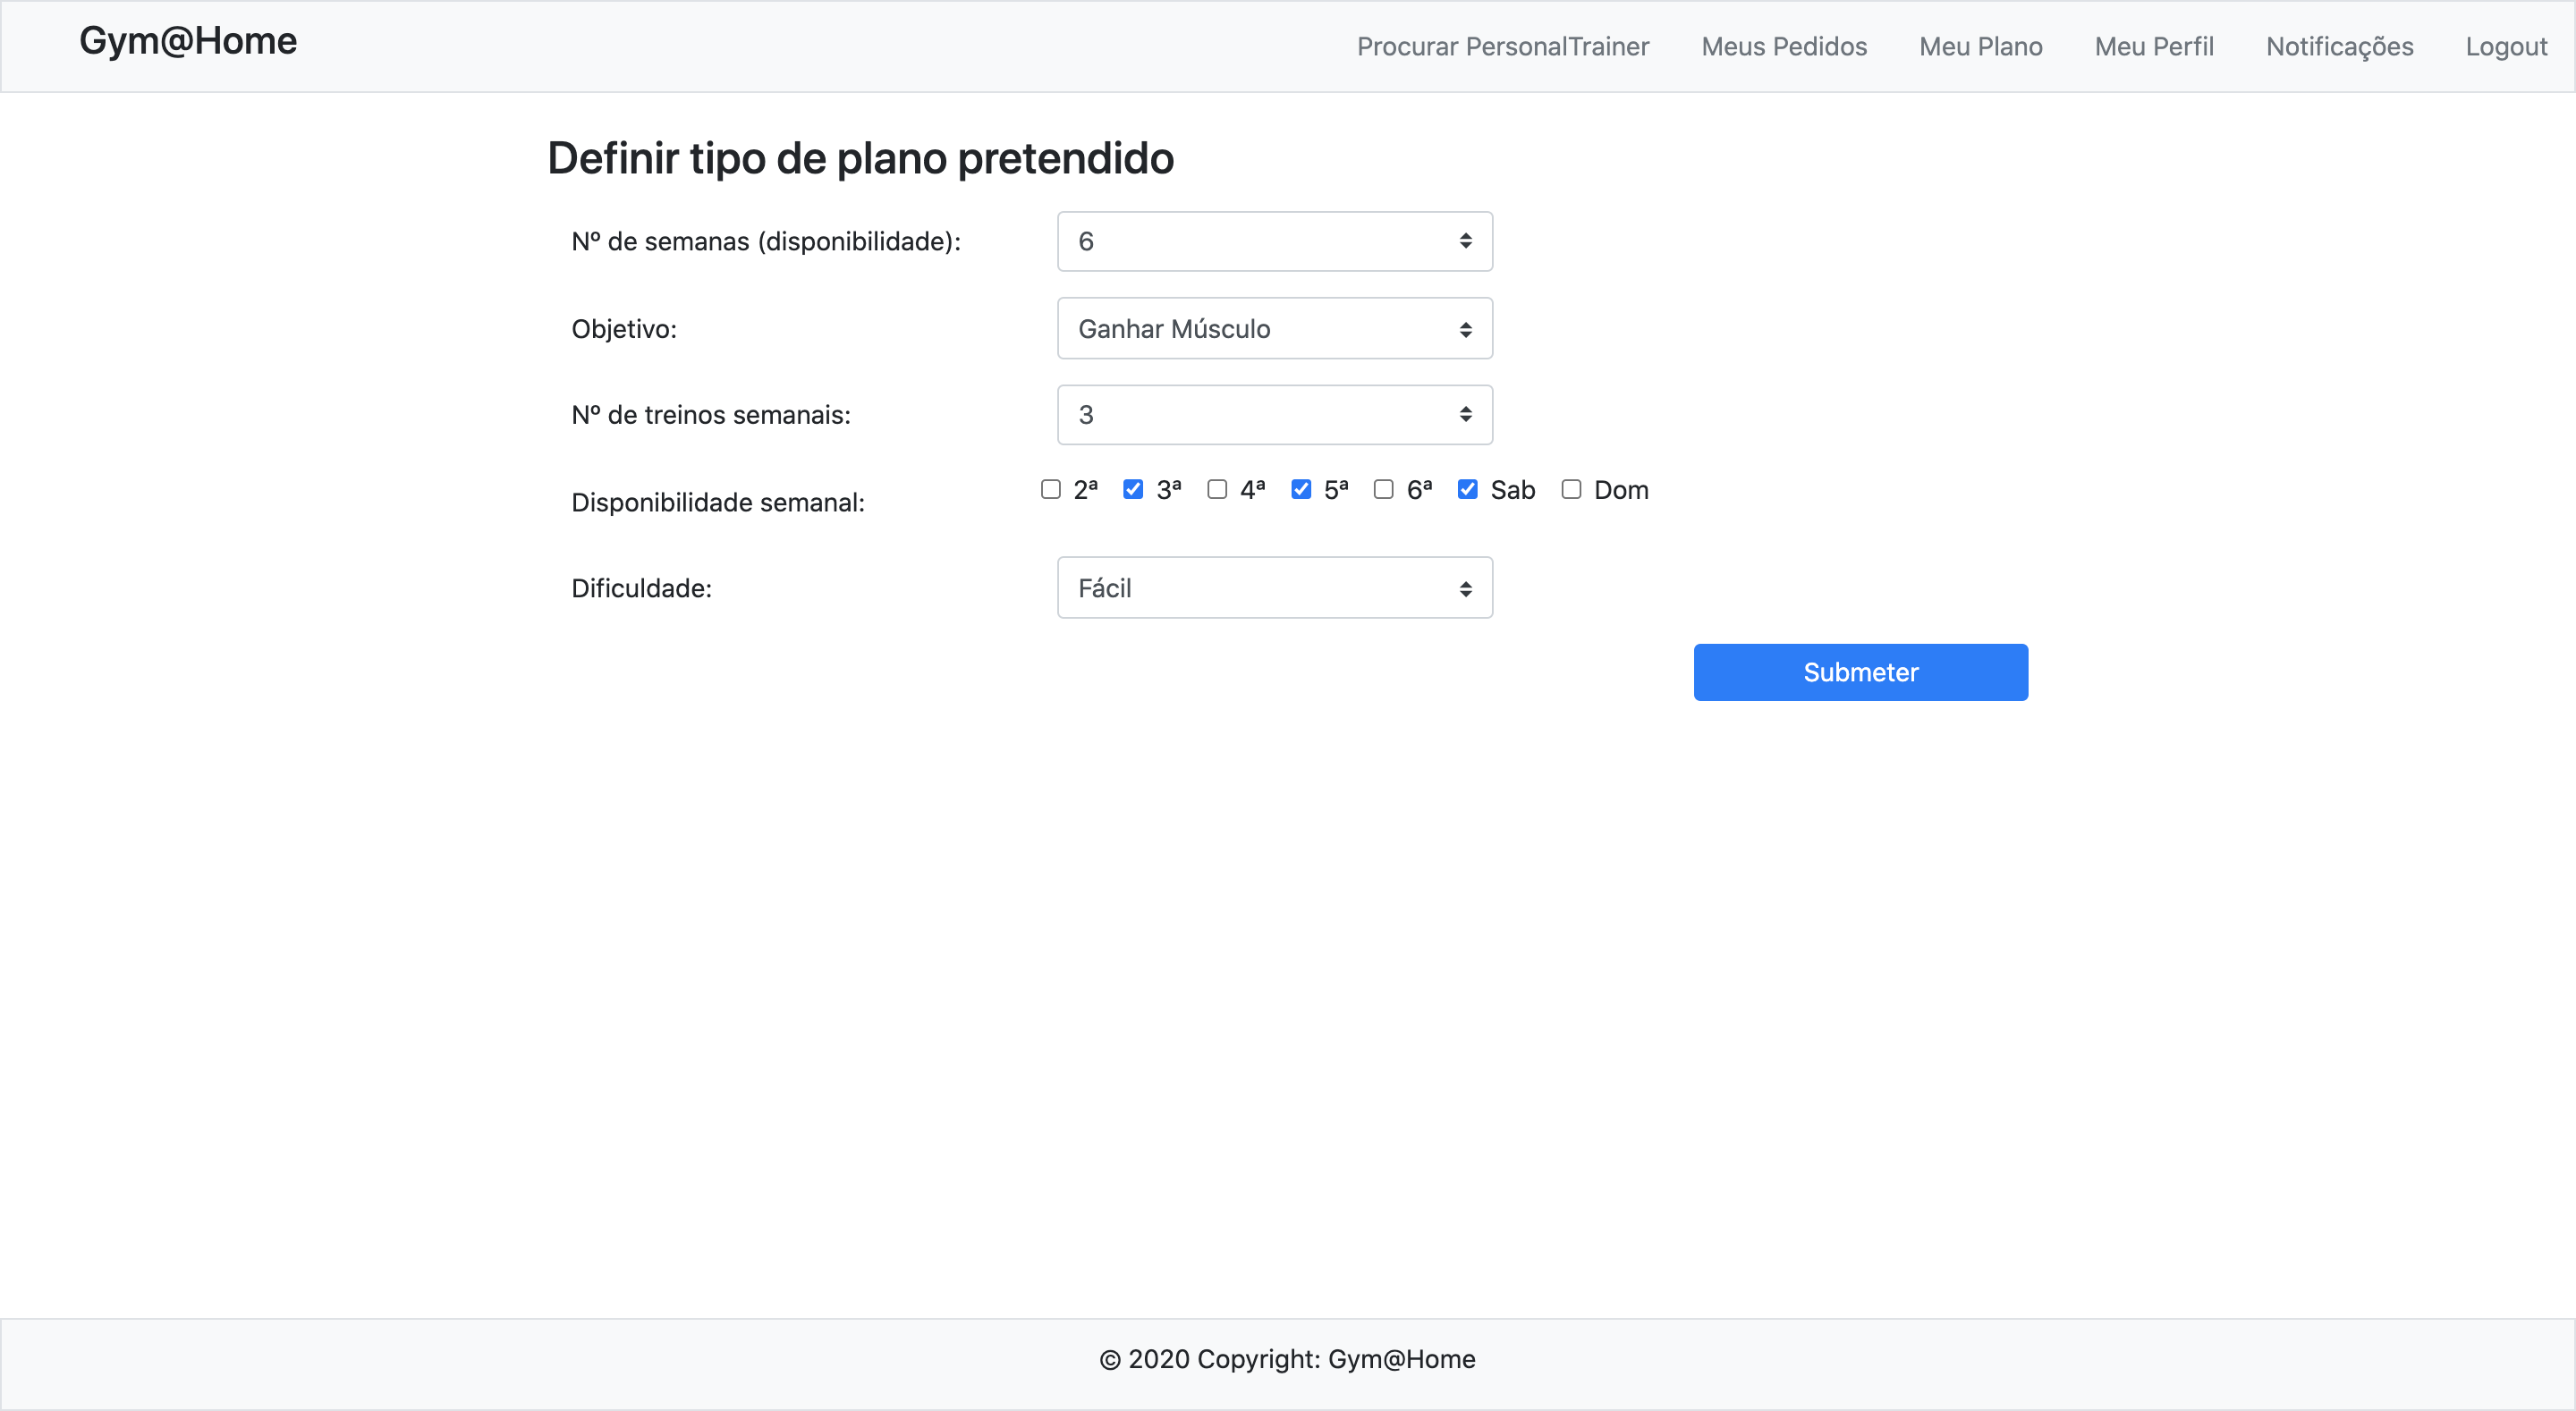
\includegraphics[scale=0.25]{images/interfaces/client_formulario.png}
    \caption{Interface Preencher Pedido.}
    \label{fig:interfacepreencherpedido}
\end{figure}

\subsubsection{Princípios de usabilidade}
\begin{itemize}
    \item \textbf{Synthesizability}: após a submissão do formulário/pedido de plano, vai ser redireccionado para a página que tem todos os pedidos enviados pelo Cliente, permitindo assim que o mesmo perceba o efeito da sua acção.
\end{itemize}

\subsubsection{Heurísticas de Normam}
\begin{itemize}
    \item \textbf{Error prevention}: Todos os inputs estão predefinidos, evitando assim erros por parte do Cliente.
    \item \textbf{Recognition rather than recall}: utilização de dropdowns permite que o utilizador não tenha que memorizar as opções existentes.
\end{itemize}

\subsection{Consultar Semana do plano}
\label{subsec:semana}

\subsubsection{Descrição}
\hspace{5mm} A mockup de visualização da Semana de um plano é comum a ambos o utilizadores, excepto que o Cliente contém um botão para avaliar o PT. Dessa forma, vamos apresentar a do Cliente, no entanto são praticamente semelhantes. 

\hspace{5mm} O Cliente consegue ver os workouts da semana, bem como verificar a sua condição física através dos seus dados biométricos. Na interface final foi acrescentada ainda uma barra do IMC com os valores de referência da OMS, informando assim o Cliente sobre o seu estado do IMC de forma mais intuitiva.

\hspace{5mm} Na tabela o Cliente pode seleccionar um workout tanto por realizar como realizado, sendo que no caso de já estar realizado não lhe é permitido realizar outra vez. Isto é possível para o Cliente poder ver as Tarefas que realizou em Workouts anteriores.

\hspace{5mm} Ainda nesta mockup contém a funcionalidade de avaliar o PT, para o cálculo da sua classificação.

\begin{figure}[H]
    \centering
    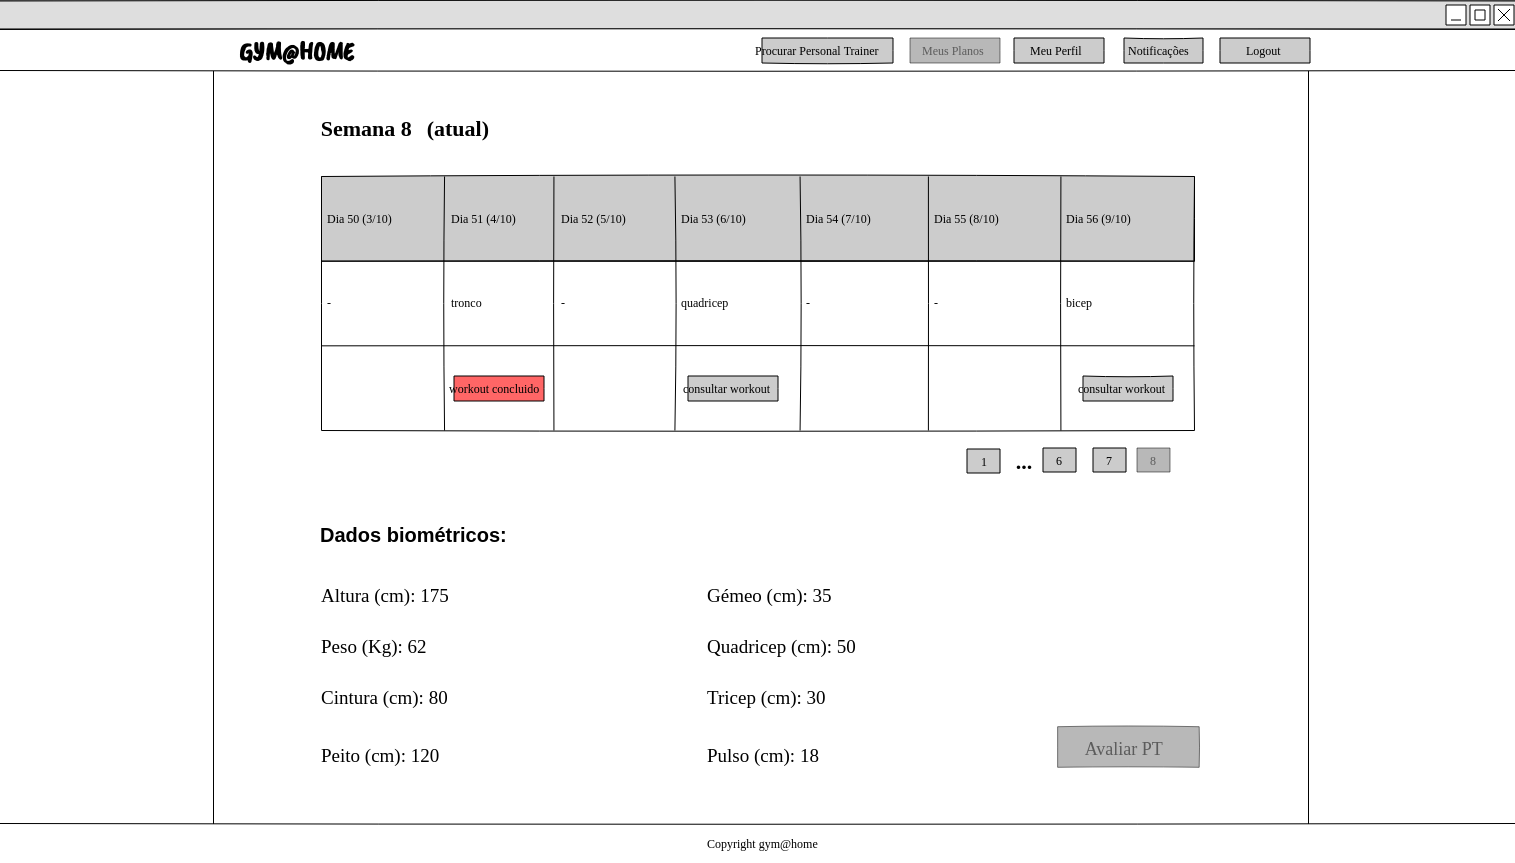
\includegraphics[scale=0.25]{images/mockups/cliente_meus_planos_semana_8_atual.png}
    \caption{Mockup Semana.}
    \label{fig:mockupsemana}
\end{figure}

\begin{figure}[H]
    \centering
    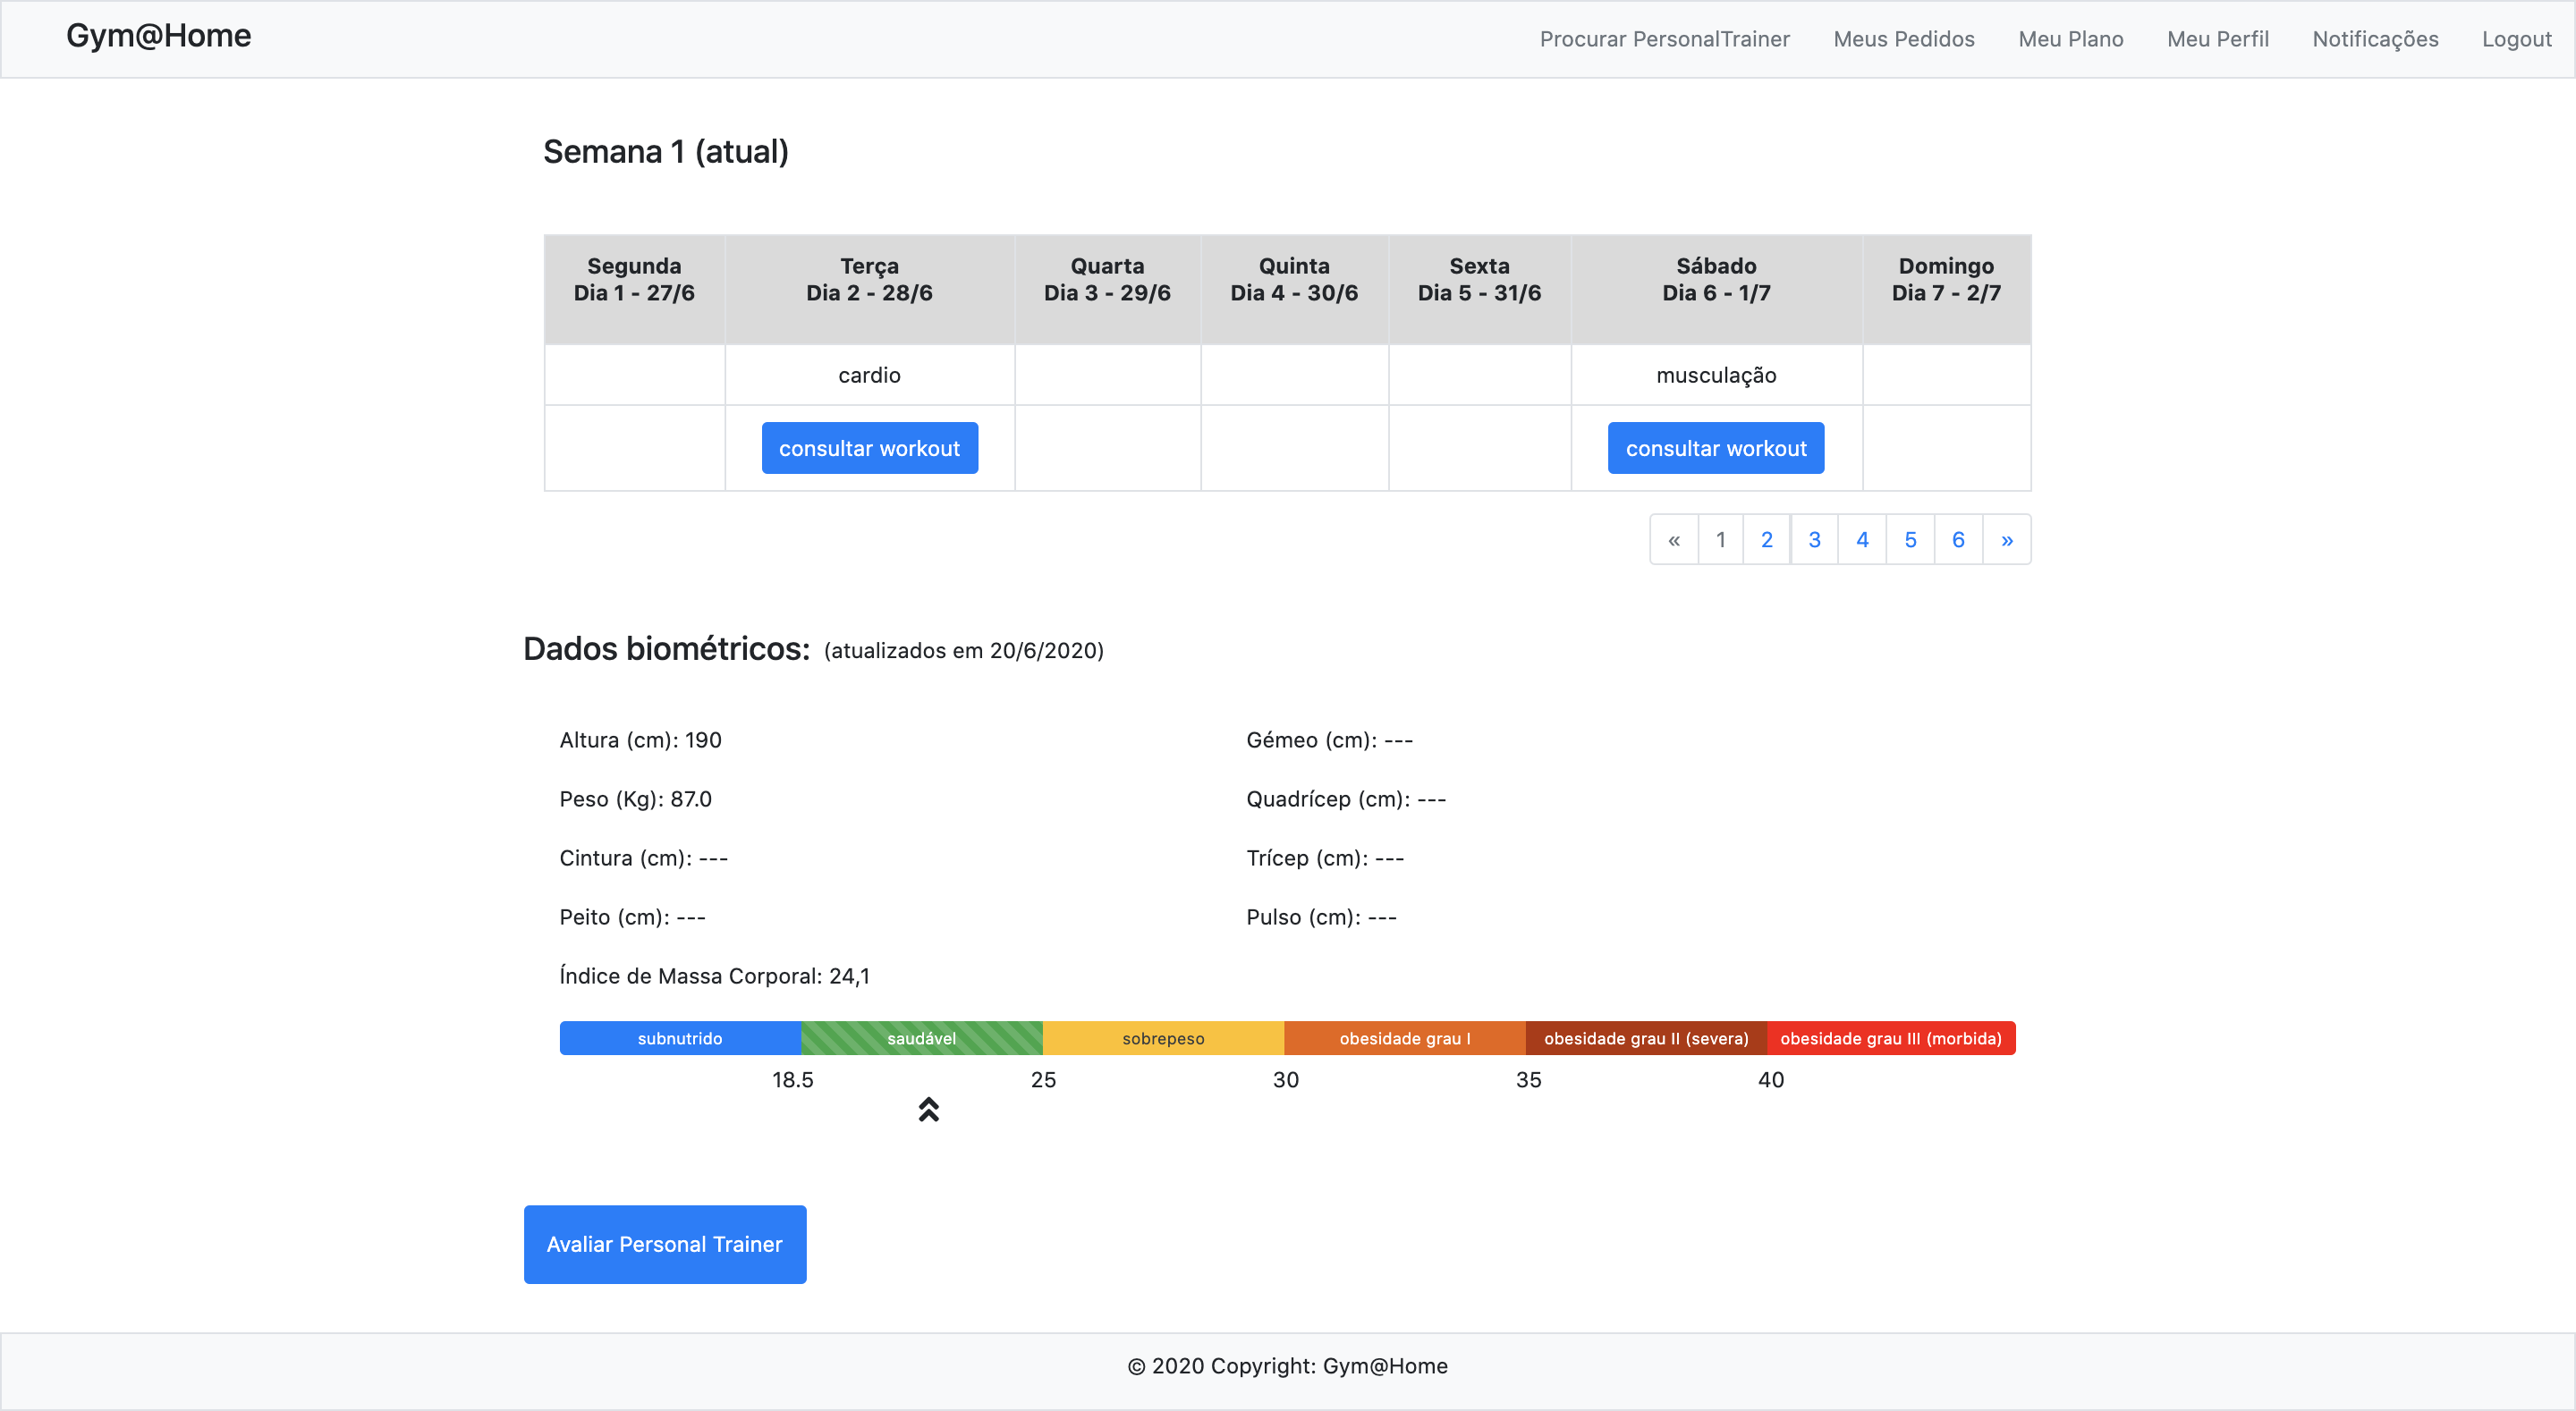
\includegraphics[scale=0.25]{images/interfaces/client_semana.png}
    \caption{Interface Semana.}
    \label{fig:interfacesemana}
\end{figure}

\subsubsection{Princípios de Usabilidade}
\begin{itemize}
    \item \textbf{Observability}: Mais especificamente \textbf{Browsability} pois o Cliente consegue navegar entre as várias semanas do seu plano.
    \item \textbf{Familiarity}: utilizou-se o formato semanal \textbf{comum}/\textbf{padrão} em horários e calendários, visto que é mais familiar aos utilizadores.
    \item \textbf{Generalizability} e \textbf{Consistency}: visto que utilizou-se a mesma estrutura tanto para a consulta pelo Cliente, bem como pelo PT, apesar de terem algumas diferenças, manteve-se a estrutura semanal, bem como os dados biométricos, excepto o botão de avaliação do PT, que não faz sentido no lado do PT.
\end{itemize}

\subsubsection{Heurísticas de Normam}
\begin{itemize}
    \item \textbf{Visibility of system status}: o utilizador conhece o estado da aplicação, como por exemplo, os \textbf{workouts} que já foram feitos, aparecem com uma cor diferente. 
    \item \textbf{Recognition rather than recall}: Os dados biométricos do Cliente são ilustrados durante a visualização da semana para o Cliente não ter de se lembrar de quais eram os valores dos dados biométricos.
    \item \textbf{Consistency and standards}: tal como foi dito em relação à \textbf{Familiarity}, sobre a estrutura semana usada, também se aplica a esta heurística relacionada com consistência e padrões.
\end{itemize}

\subsection{Consultar Workout}
\label{subsec:workout}

\subsubsection{Descrição}
\hspace{5mm} Da mesma forma que o anterior, este mockup também é bastante semelhante a ambos os utilizadores, pelo que apresentar-se-á apenas a view do Cliente. Nesta mockup o Cliente vê uma Tarefa de cada vez, com a listagem das séries e toda a informação necessário sobre a Tarefa. Aqui pode avançar e recuar nas tarefas, sendo que na última Tarefa do Workout pode terminar o Workout.

\begin{figure}[H]
    \centering
    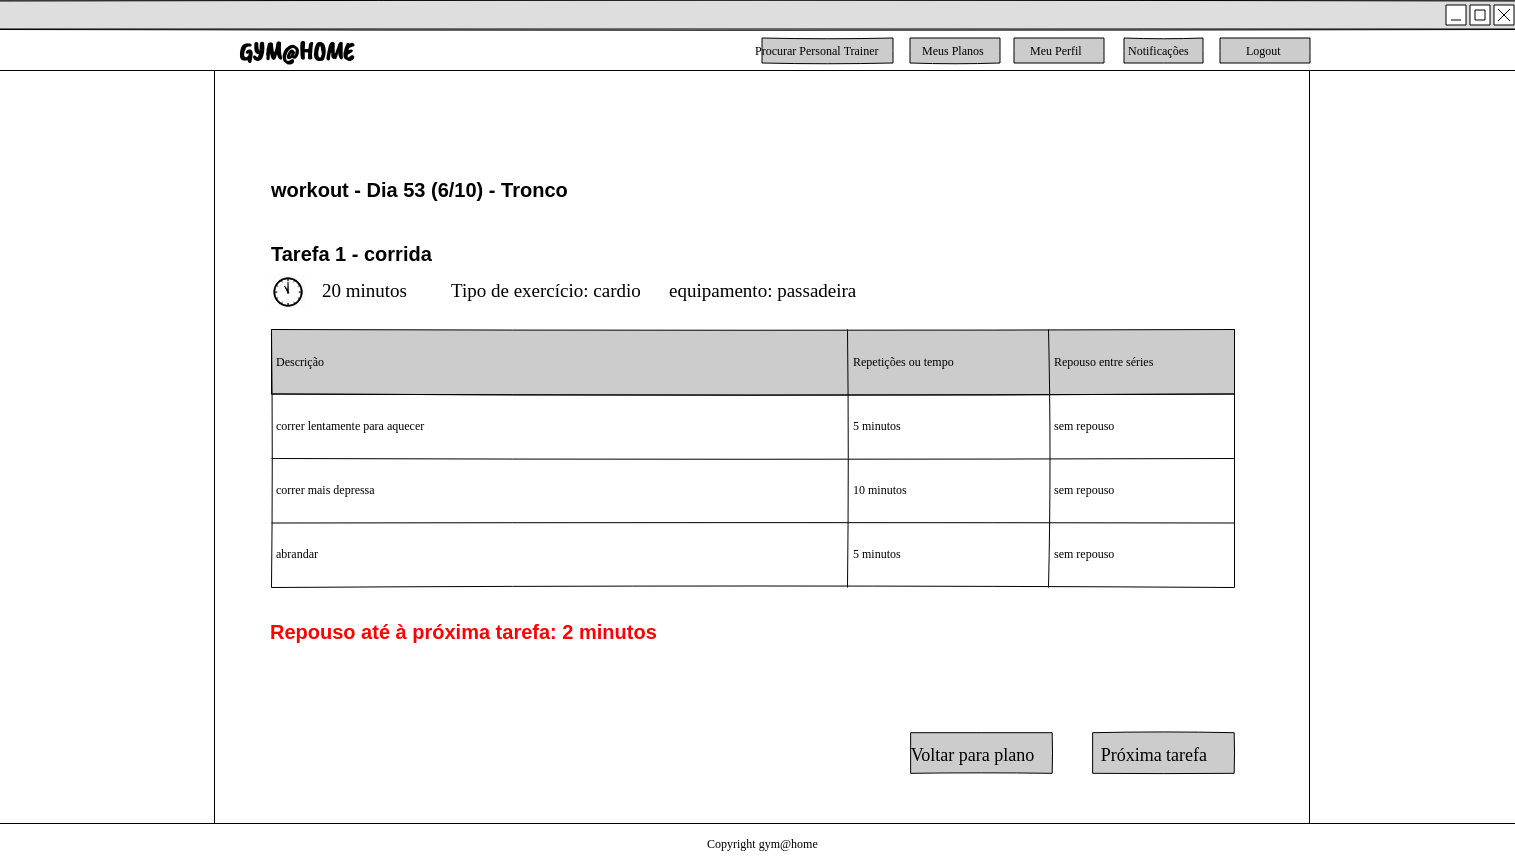
\includegraphics[scale=0.25]{images/mockups/cliente_plano_tarefa_1.png}
    \caption{Mockup Workout.}
    \label{fig:mockupworkout}
\end{figure}

\begin{figure}[H]
    \centering
    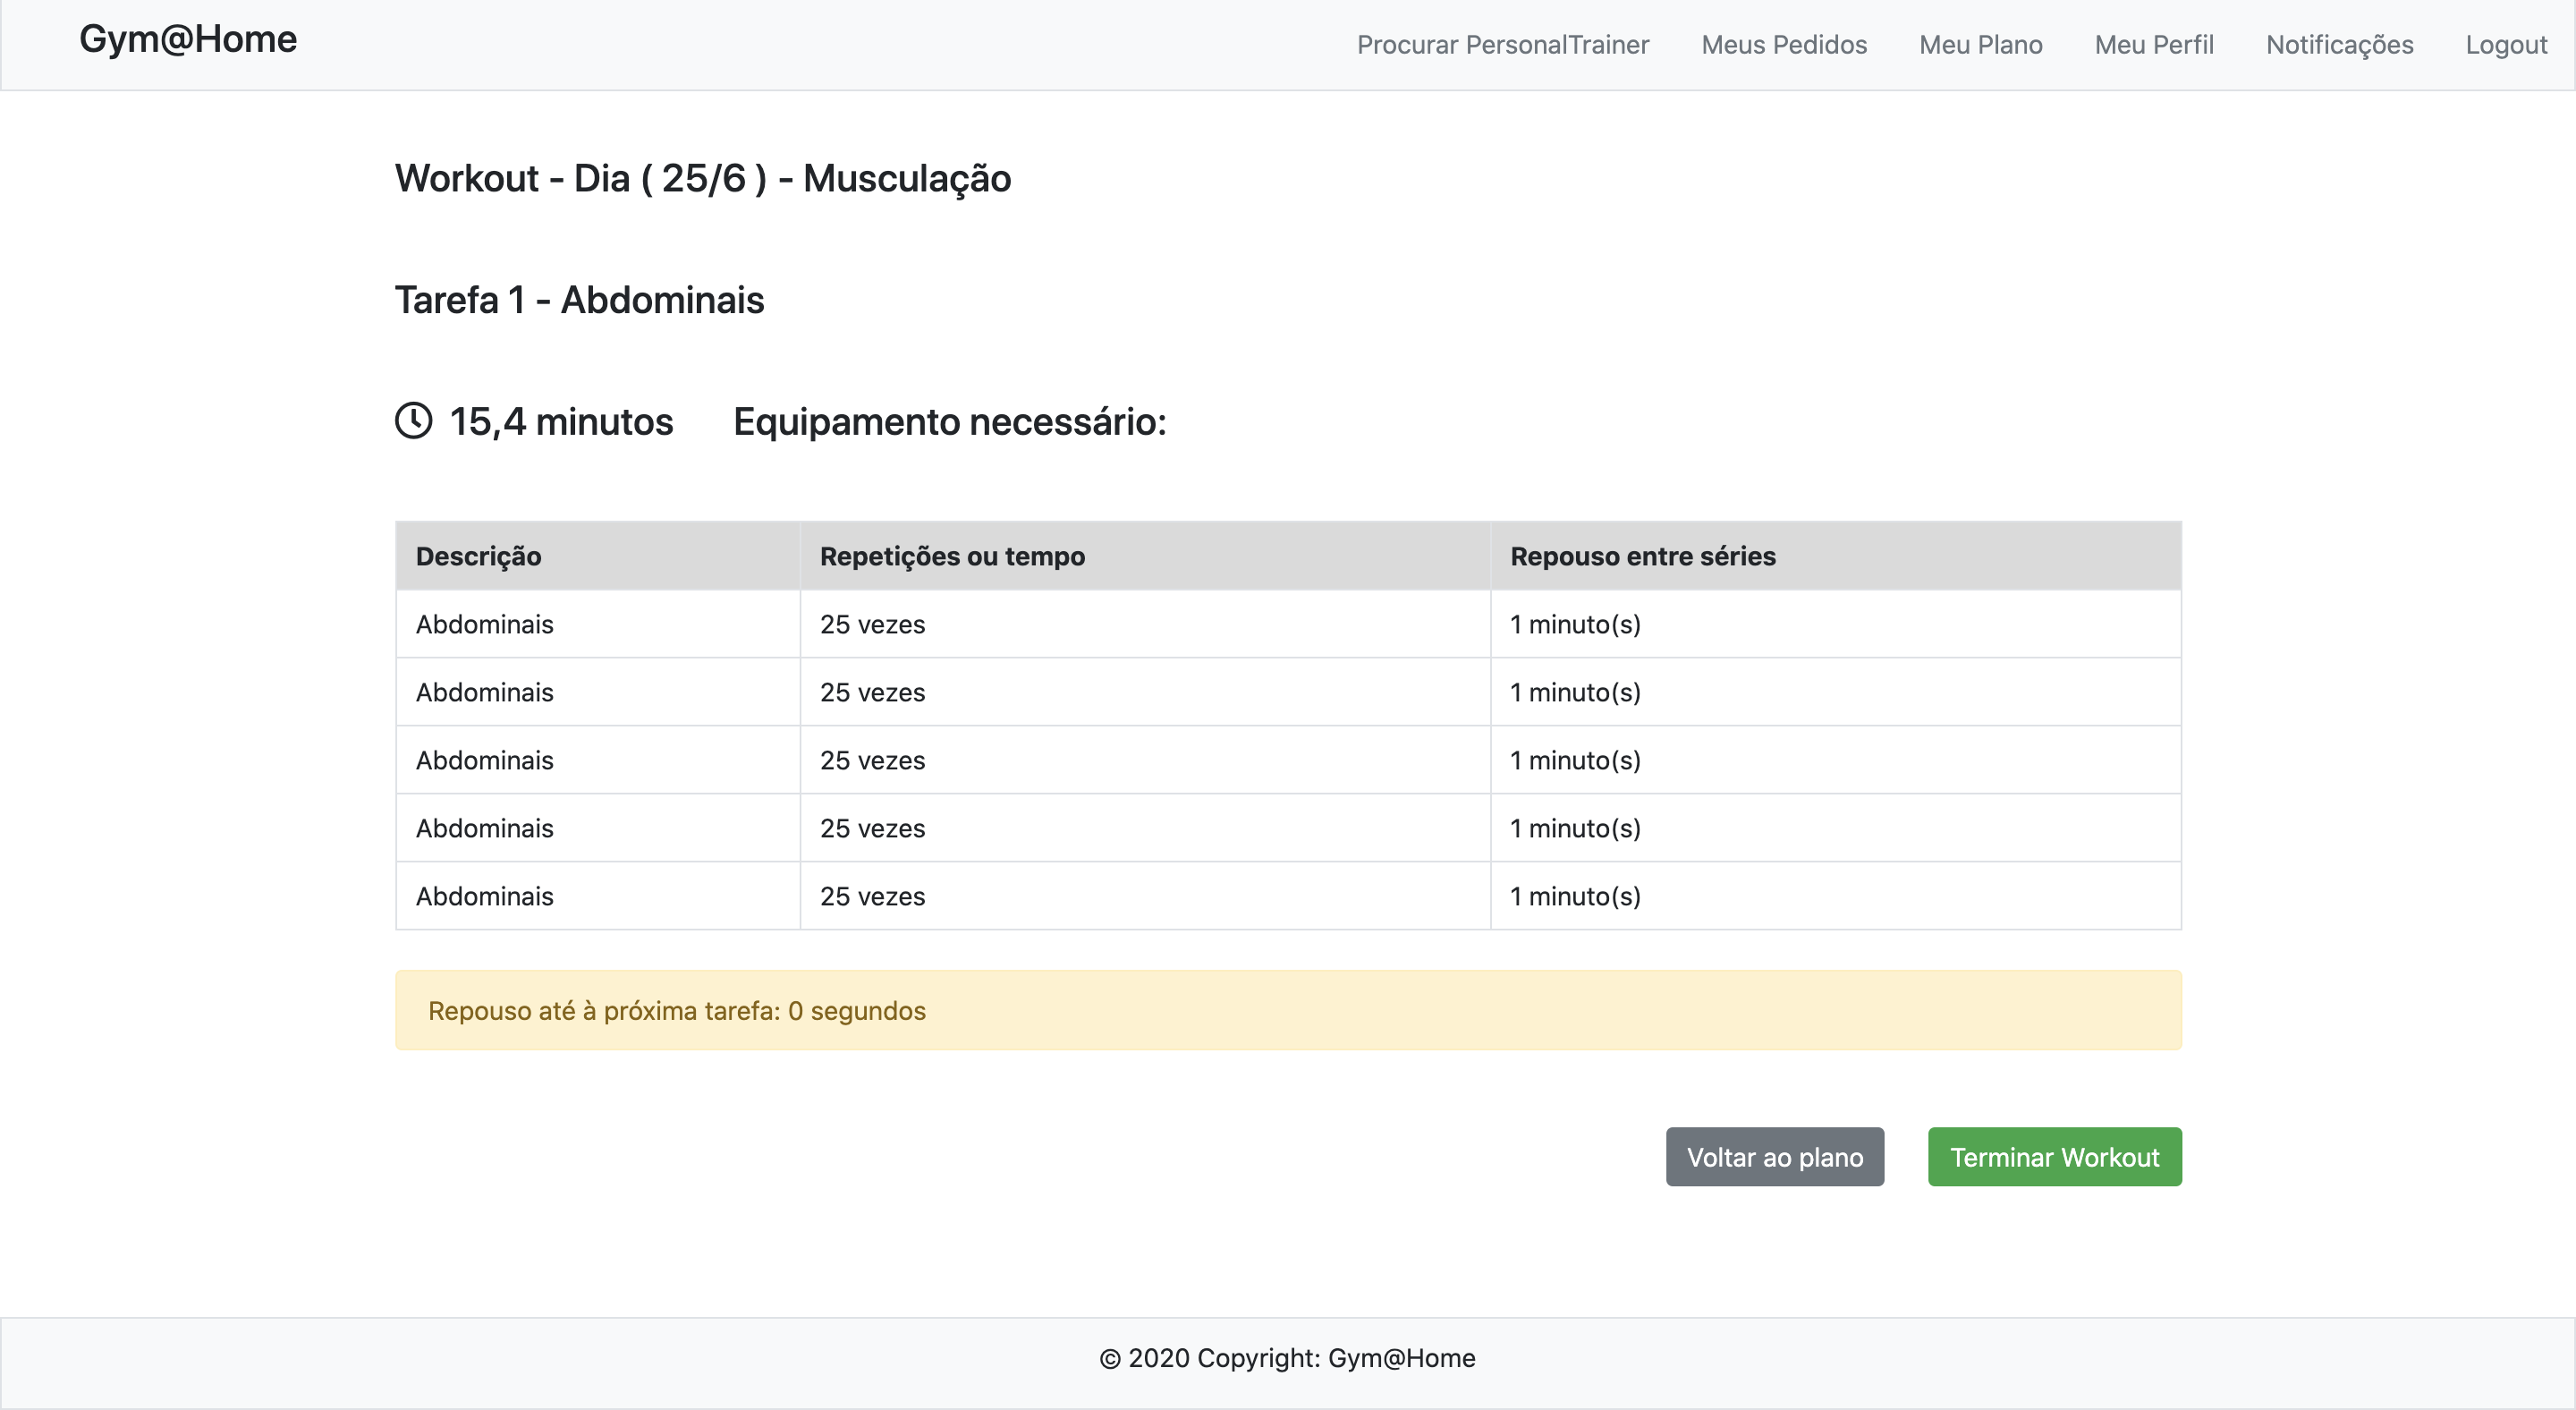
\includegraphics[scale=0.25]{images/interfaces/client_workout.png}
    \caption{Interface Workout.}
    \label{fig:interfaceworkout}
\end{figure}

\subsubsection{Princípios de usabilidade}
\begin{itemize}
    \item \textbf{Observability}: Mais especificamente \textbf{Browsability} pois o Cliente consegue navegar entre as várias tarefas de um workout.
    
    \item \textbf{Generalizability} e \textbf{Consistency}: visto que utilizou-se a mesma estrutura tanto para a consulta pelo Cliente, bem como pelo PT, apesar de terem algumas diferenças, manteve-se a estrutura tabelar das séries de uma tarefa, bem como as informações da tarefa, considerando-se assim que torna-se genérica para ambos os utilizadores.
\end{itemize}

\subsubsection{Heurísticas de Normam}
\begin{itemize}
    \item \textbf{Recognition rather than recall}: as informações sobre o dia da semana e a definição do workout são passadas para esta view para que o cliente/PT não necessitem de memorizar.
\end{itemize}

\subsection{Pedidos enviados pelo Cliente}
\label{subsec:pedidos}

\subsubsection{Descrição}
\hspace{5mm} A interface Pedidos enviados pelo Cliente foi adicionada posteriormente ao desenho das mockups, pelo que só existe a interface final. Nesta interface o Cliente poderá ver todos os pedidos que já realizou, sendo apresentadas todas as informações do pedido, tais como o seu estado (aceite, rejeitado ou pedente), nome do PT, dados do formulário preenchido e ainda a possibilidade de ver o perfil do PT ao qual o pedido foi direccionado.

\begin{figure}[H]
    \centering
    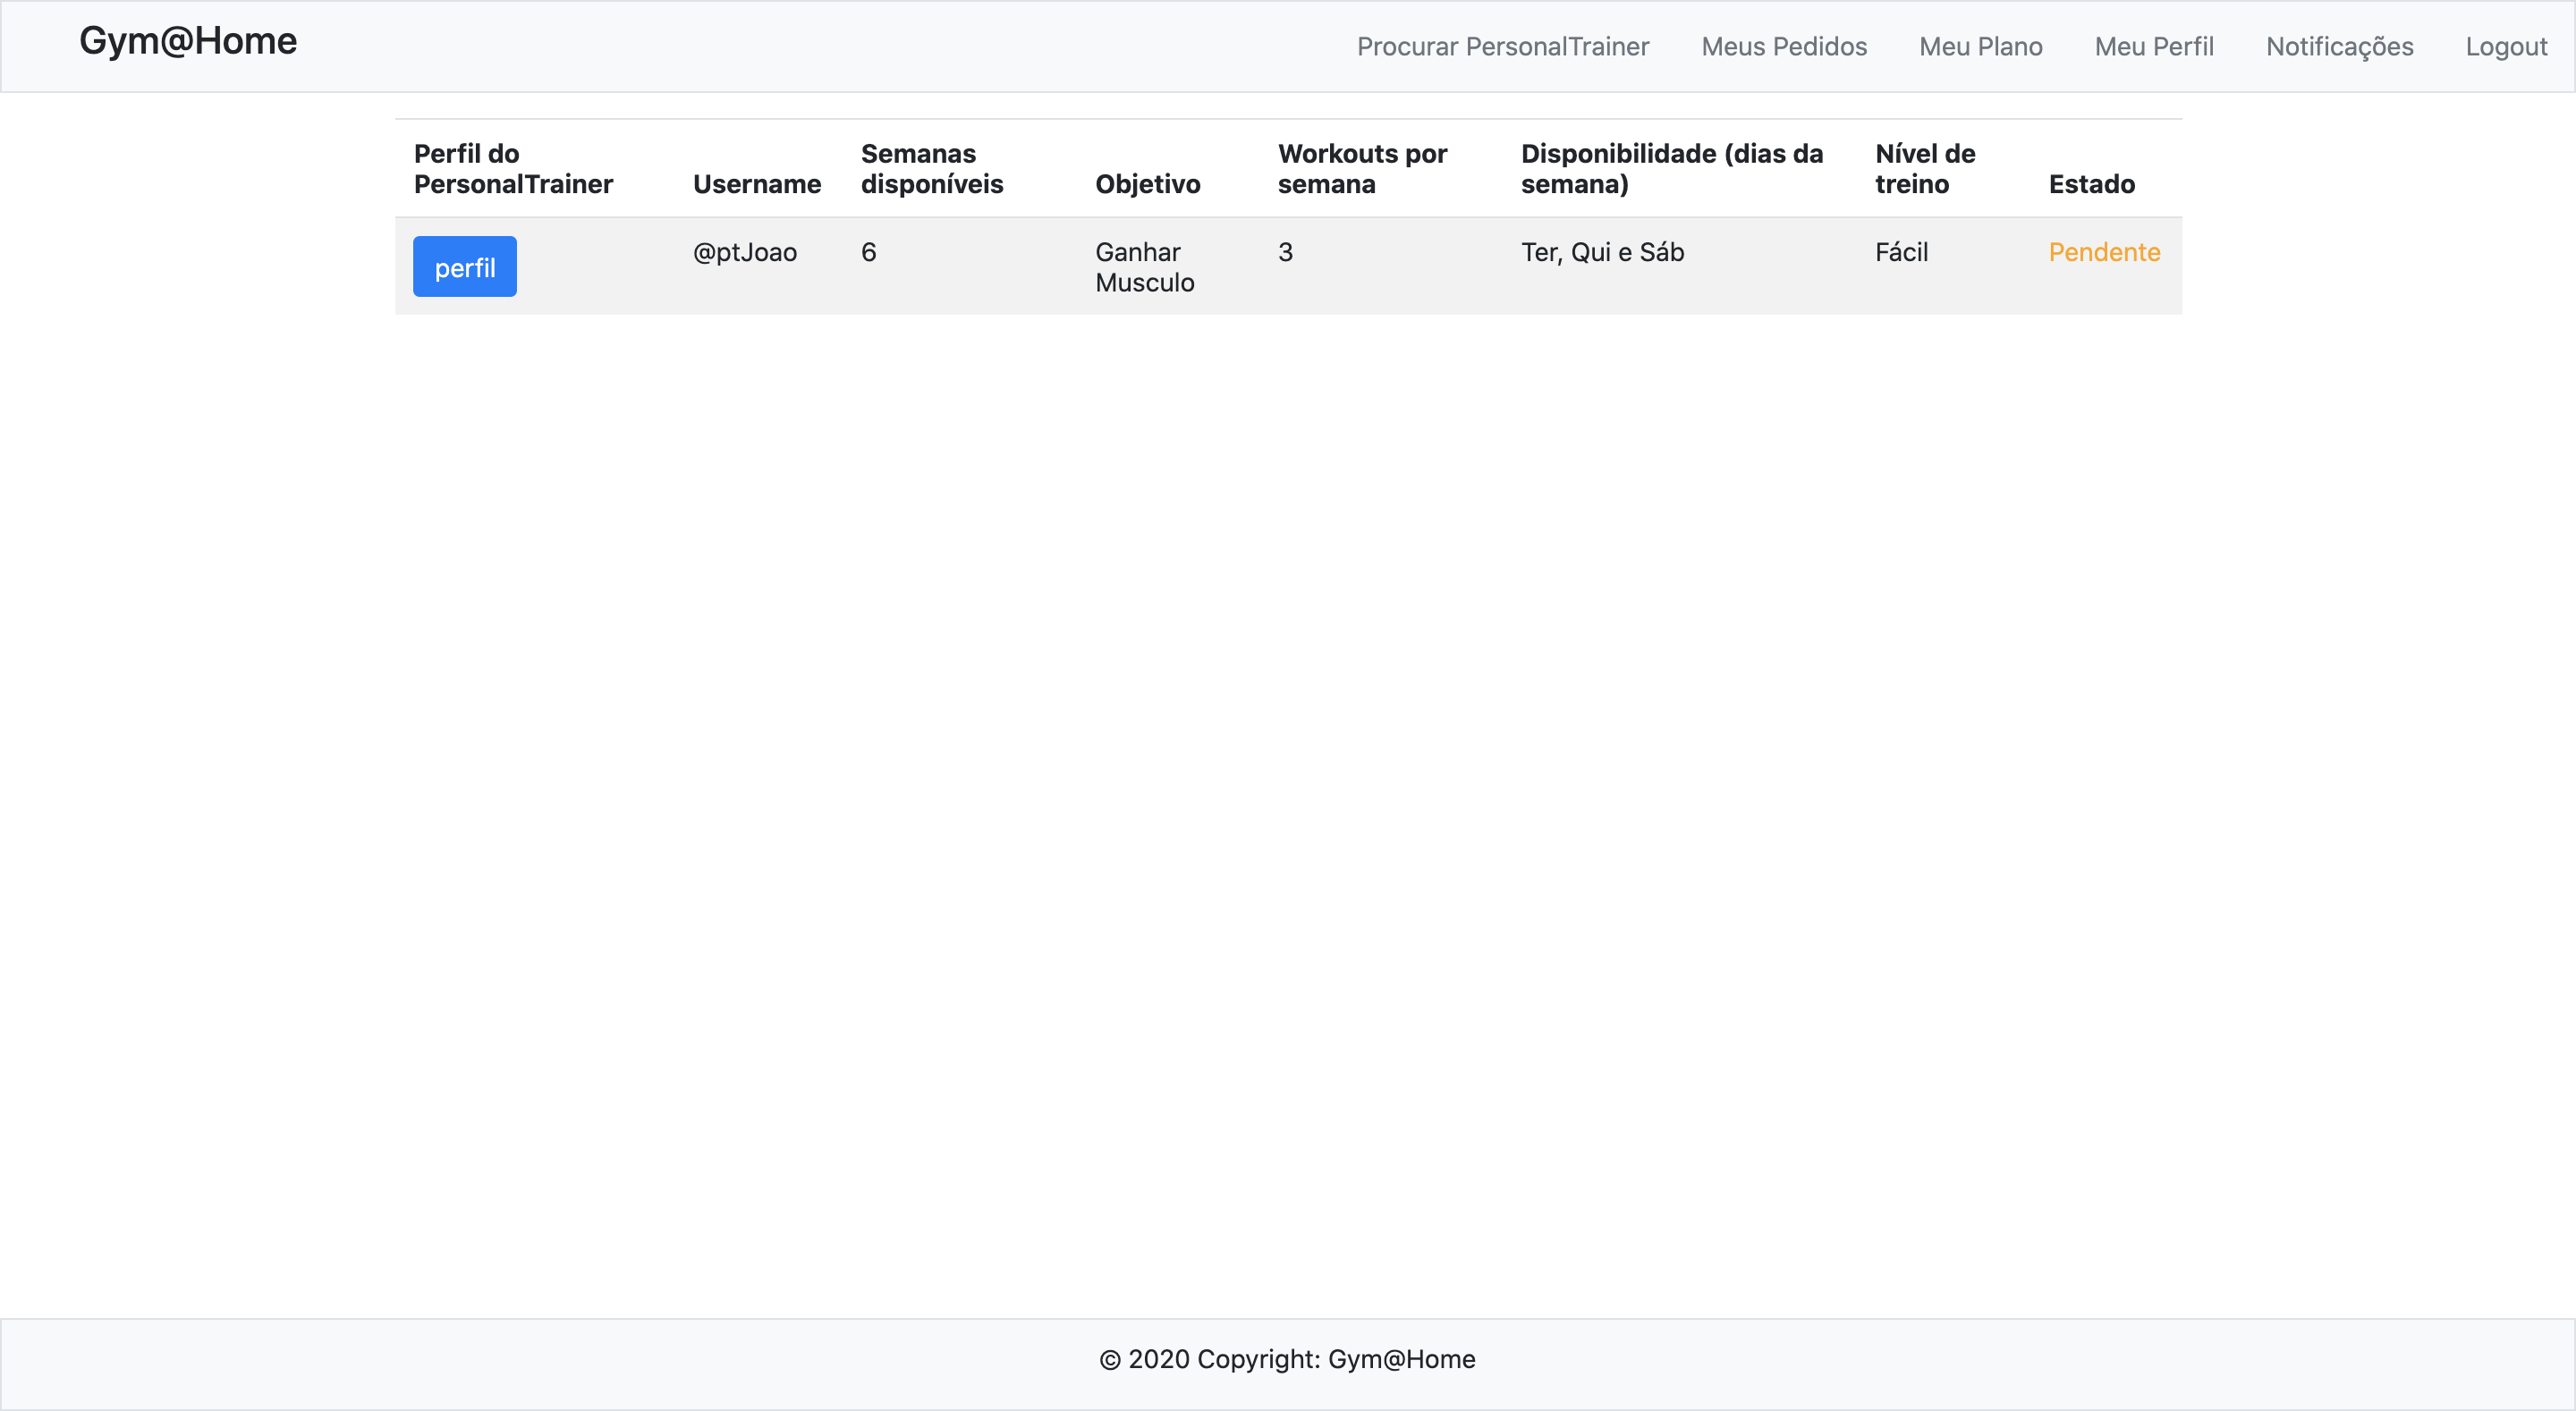
\includegraphics[scale=0.25]{images/interfaces/client_meus_pedidos.png}
    \caption{Interface Pedidos.}
    \label{fig:interfacepedidos}
\end{figure}

\subsubsection{Princípios de usabilidade}
\begin{itemize}
    \item \textbf{Synthesizability}: a acção possível nesta interface consiste em consultar o perfil do PT, pelo que após clicar no botão "perfil", aparece um pop-up com as informações do mesmo, ou seja, o cliente consegue perceber o efeito das suas acções.
    \item \textbf{Generalizability} e \textbf{Consistency}: o PT também contem uma interface para ver os pedidos enviados para o mesmo, que a nível de estrutura pode-se considerar bastante semelhante, difere apenas no conteúdos de algumas colunas, pelo que se pode considerar que se trata de uma interface genérica no sistema. 
    \item \textbf{Observability}: esta interface pode aumentar bastante o número de linhas da tabela, no entanto cada linha tem os botões para as acções desse pedido, o que significa que se houvesse uma tabela gigante, as acções possíveis estariam lá, não necessitando de subir a página ou outra forma para encontrar os botões. No entanto o grupo reconhece que aqui também seria um bom candidato a paginação, não sendo possível implementar face à falta de tempo, mas será uma boa actualização no futuro.
\end{itemize}

\subsubsection{Heurísticas de Normam}
\begin{itemize}
    \item \textbf{Recognition rather than recall}: o cliente não precisa de memorizar o que preencheu no formulário quando enviou o pedido, pois pode consultar na tabela esses mesmos campos.
    \item \textbf{Flexibility and efficiency of use}: o botão "perfil", que mostra as informações do PT torna esse processo de consulta mais \textbf{eficiente}, como uma espécie de atalho.
\end{itemize}

\subsection{Avaliar PT}
\label{subsec:avaliarpt}

\subsubsection{Descrição}
\hspace{5mm} A qualquer momento o Cliente pode avaliar o PT pelo seu trabalho, sendo pedido uma classificação de 1 a 5 estrelas, estas avaliações serão usadas posteriormente como parâmetro para escolher ou não um PT.

\begin{figure}[H]
    \centering
    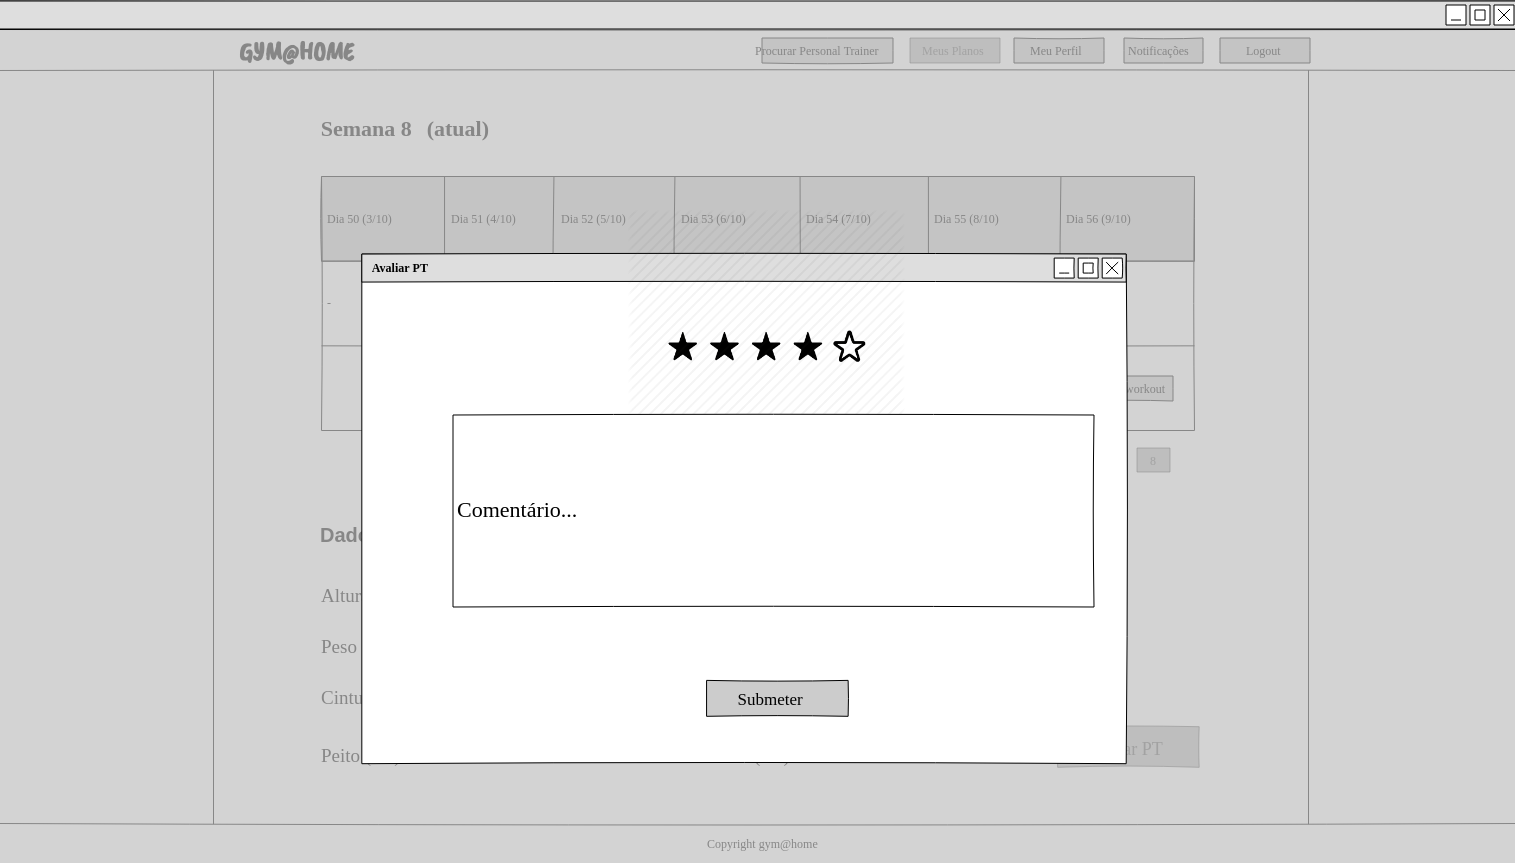
\includegraphics[scale=0.25]{images/mockups/cliente_avaliar_pt.png}
    \caption{Mockup Avaliar PT.}
    \label{fig:mockupavaliarpt}
\end{figure}

\begin{figure}[H]
    \centering
    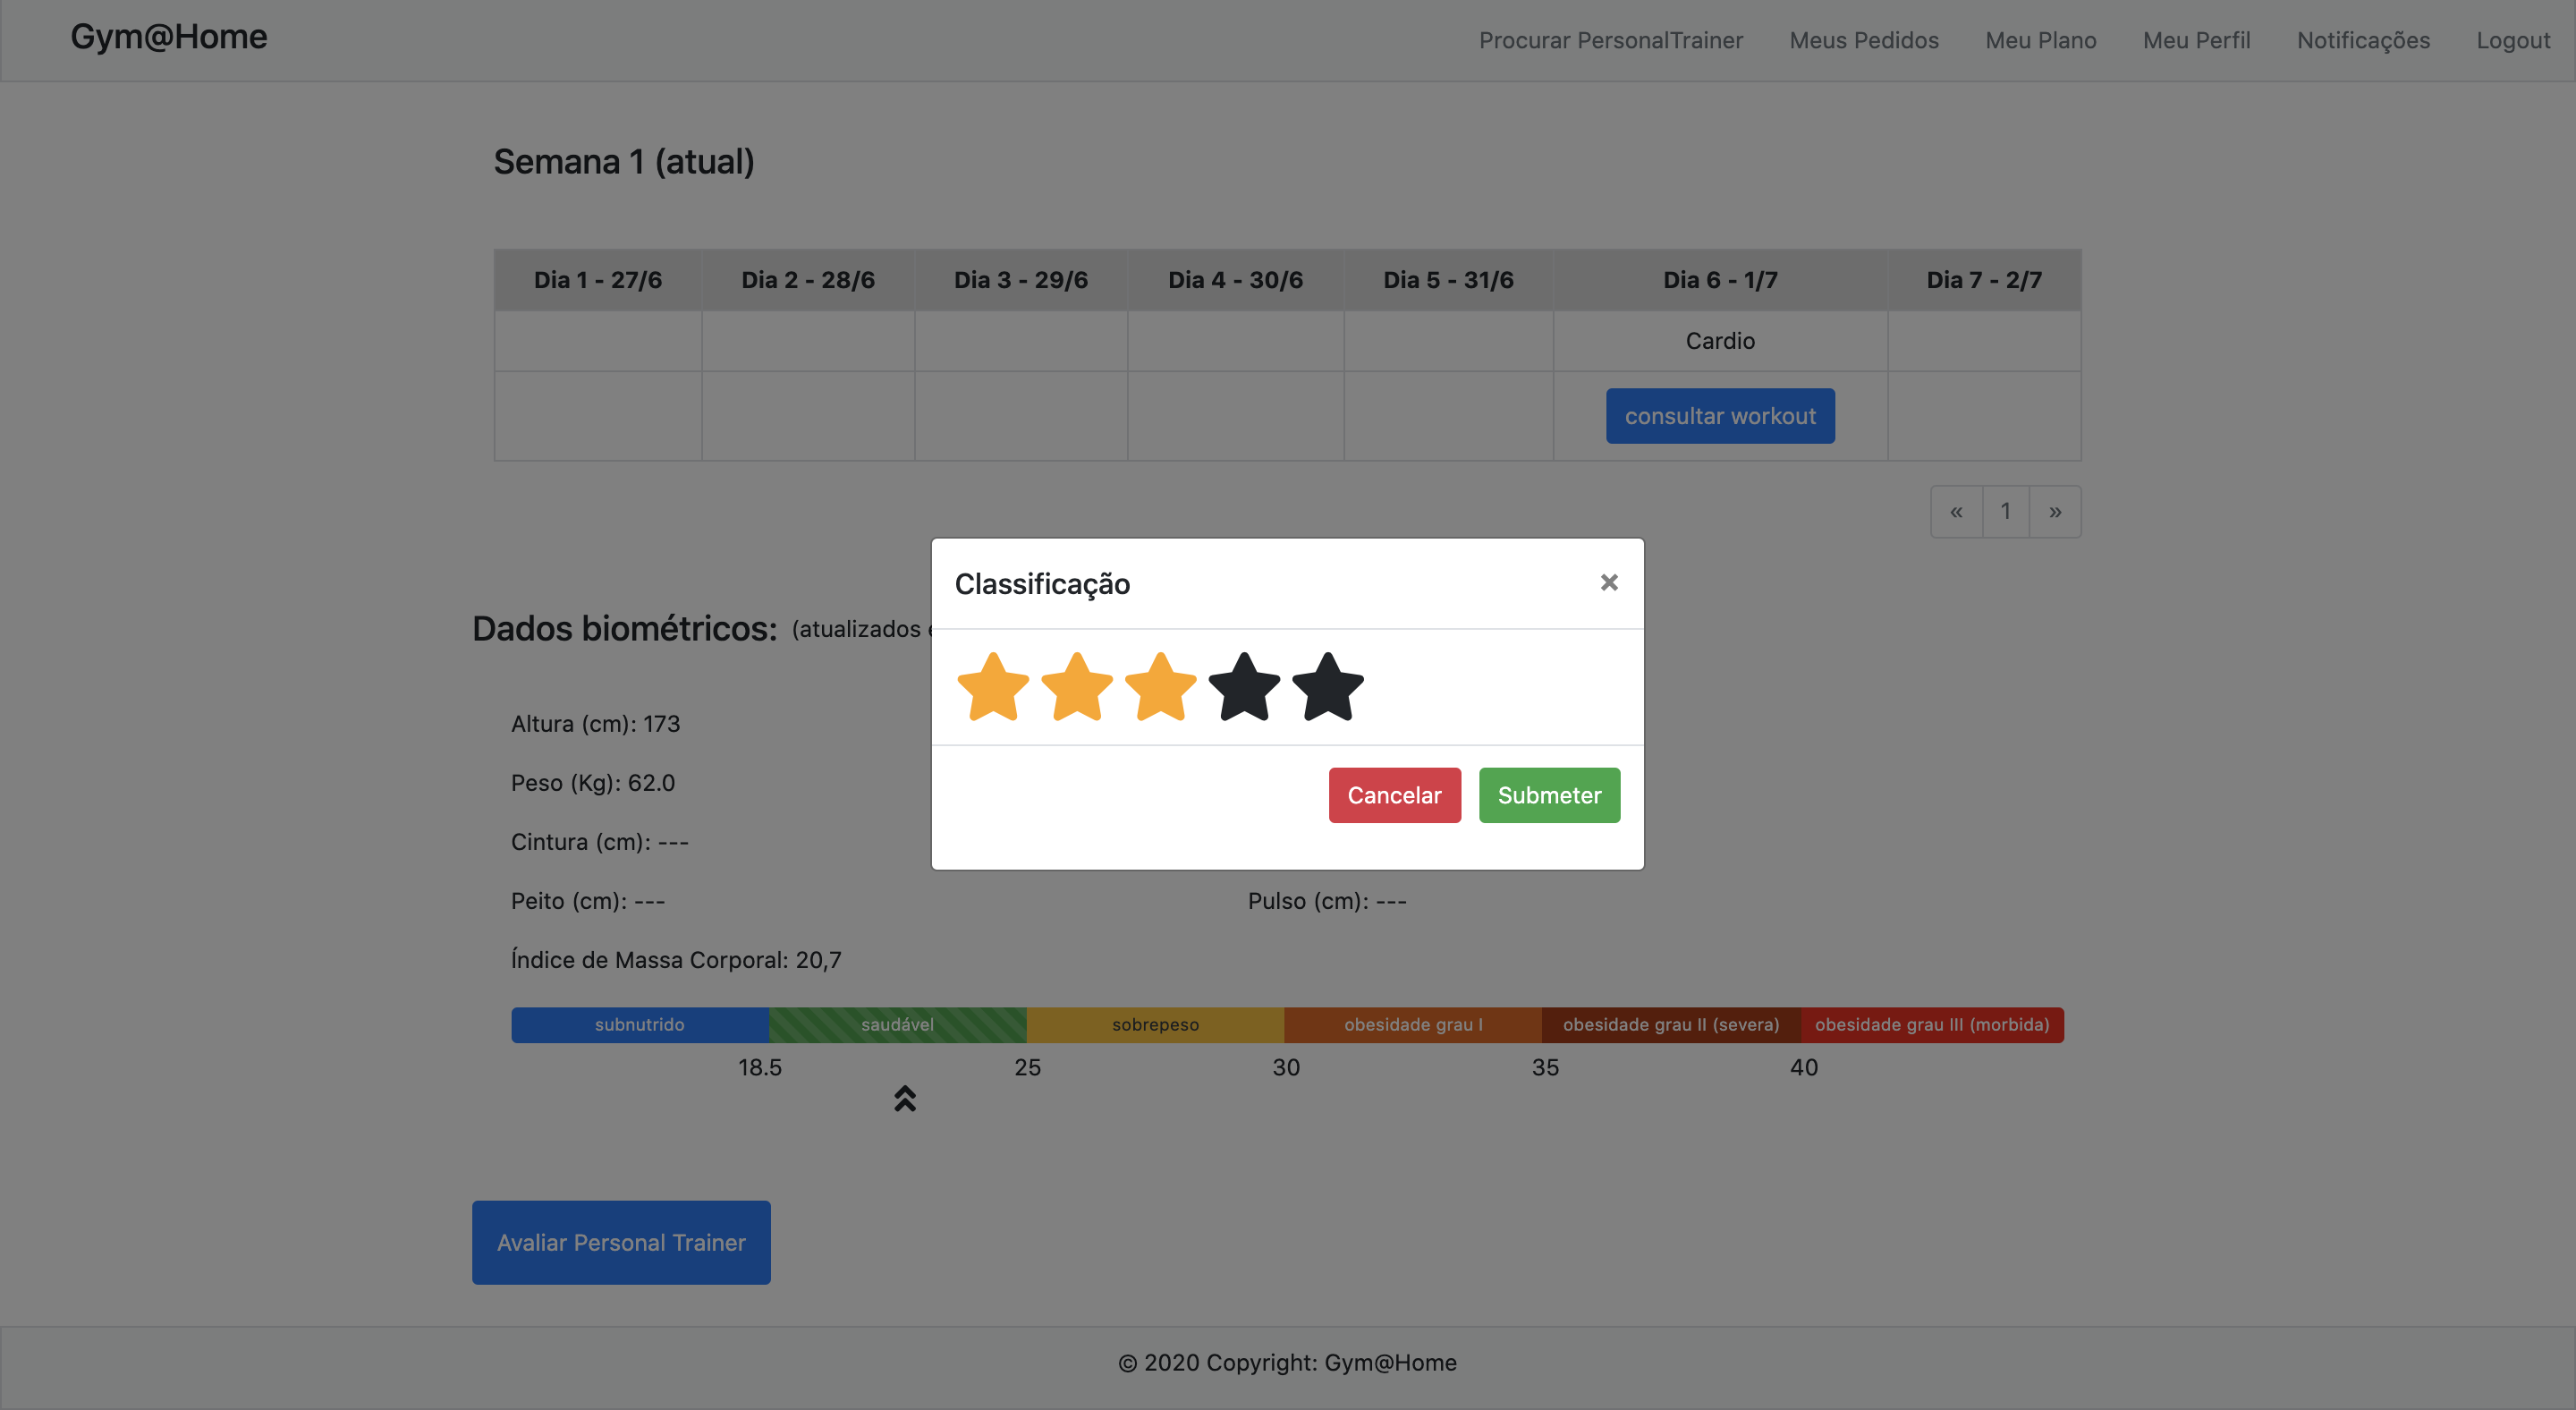
\includegraphics[scale=0.25]{images/interfaces/client_avaliar_pt.png}
    \caption{Interface Avaliar PT.}
    \label{fig:interfaceavaliarpt}
\end{figure}

\subsubsection{Princípios de usabilidade}
\begin{itemize}
    \item \textbf{Familiarity} e \textbf{Consistency}: usou-se uma forma padrão para as avaliações, através de cinco estrelas onde o utilizador selecciona.
\end{itemize}

\subsubsection{Heurísticas de Normam}
\begin{itemize}
    \item \textbf{Error prevetion}: a avaliação é inicializada com pelo menos uma estrela seleccionada, para evitar que o utilizador pudesse enviar zero estrelas, visto que a escala vai de um a cinco.
    \item \textbf{Consistency and standards}: tal como foi dito anteriormente, segue os princípios de \textbf{Familiarity} e \textbf{Consistency}, pelo que significa que também segue esta heurística relacionada com \textbf{padrões}.
\end{itemize}

%--------------------------------------------------------------------------%

\section{Interfaces PTs}
\label{sec:mockupspts}

\subsection{Registar PT}
\label{subsec:registarpt}

\subsubsection{Descrição}
\hspace{5mm} Tal como no registo Cliente são pedidos alguns dados obrigatórios, sendo que o PT não tem dados opcionais.

\begin{figure}[H]
    \centering
    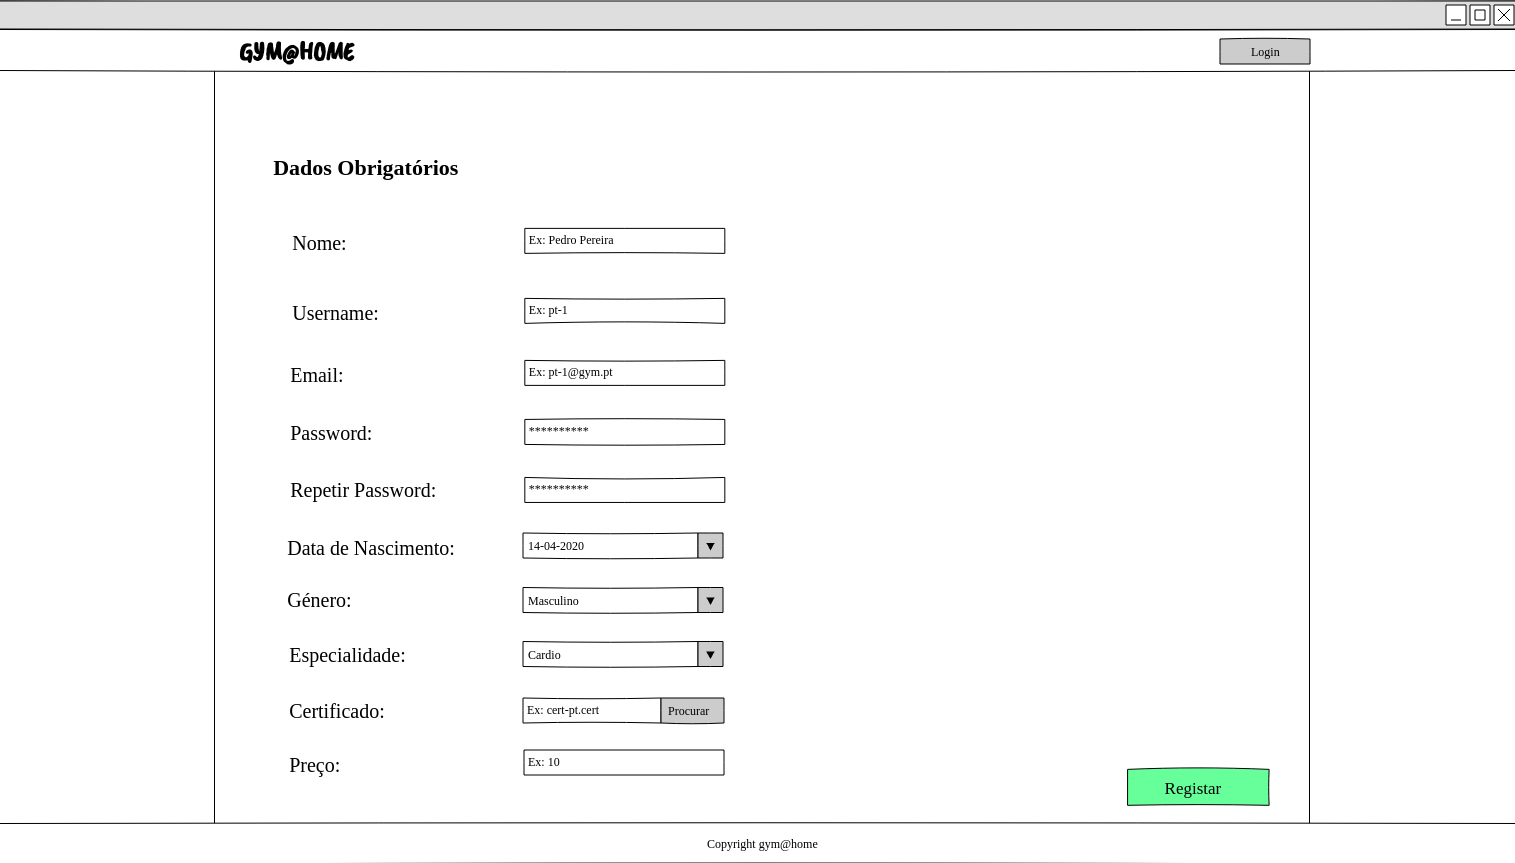
\includegraphics[scale=0.25]{images/mockups/pt_registo.png}
    \caption{Mockup Registar PT.}
    \label{fig:mockupregistarpt}
\end{figure}

\begin{figure}[H]
    \centering
    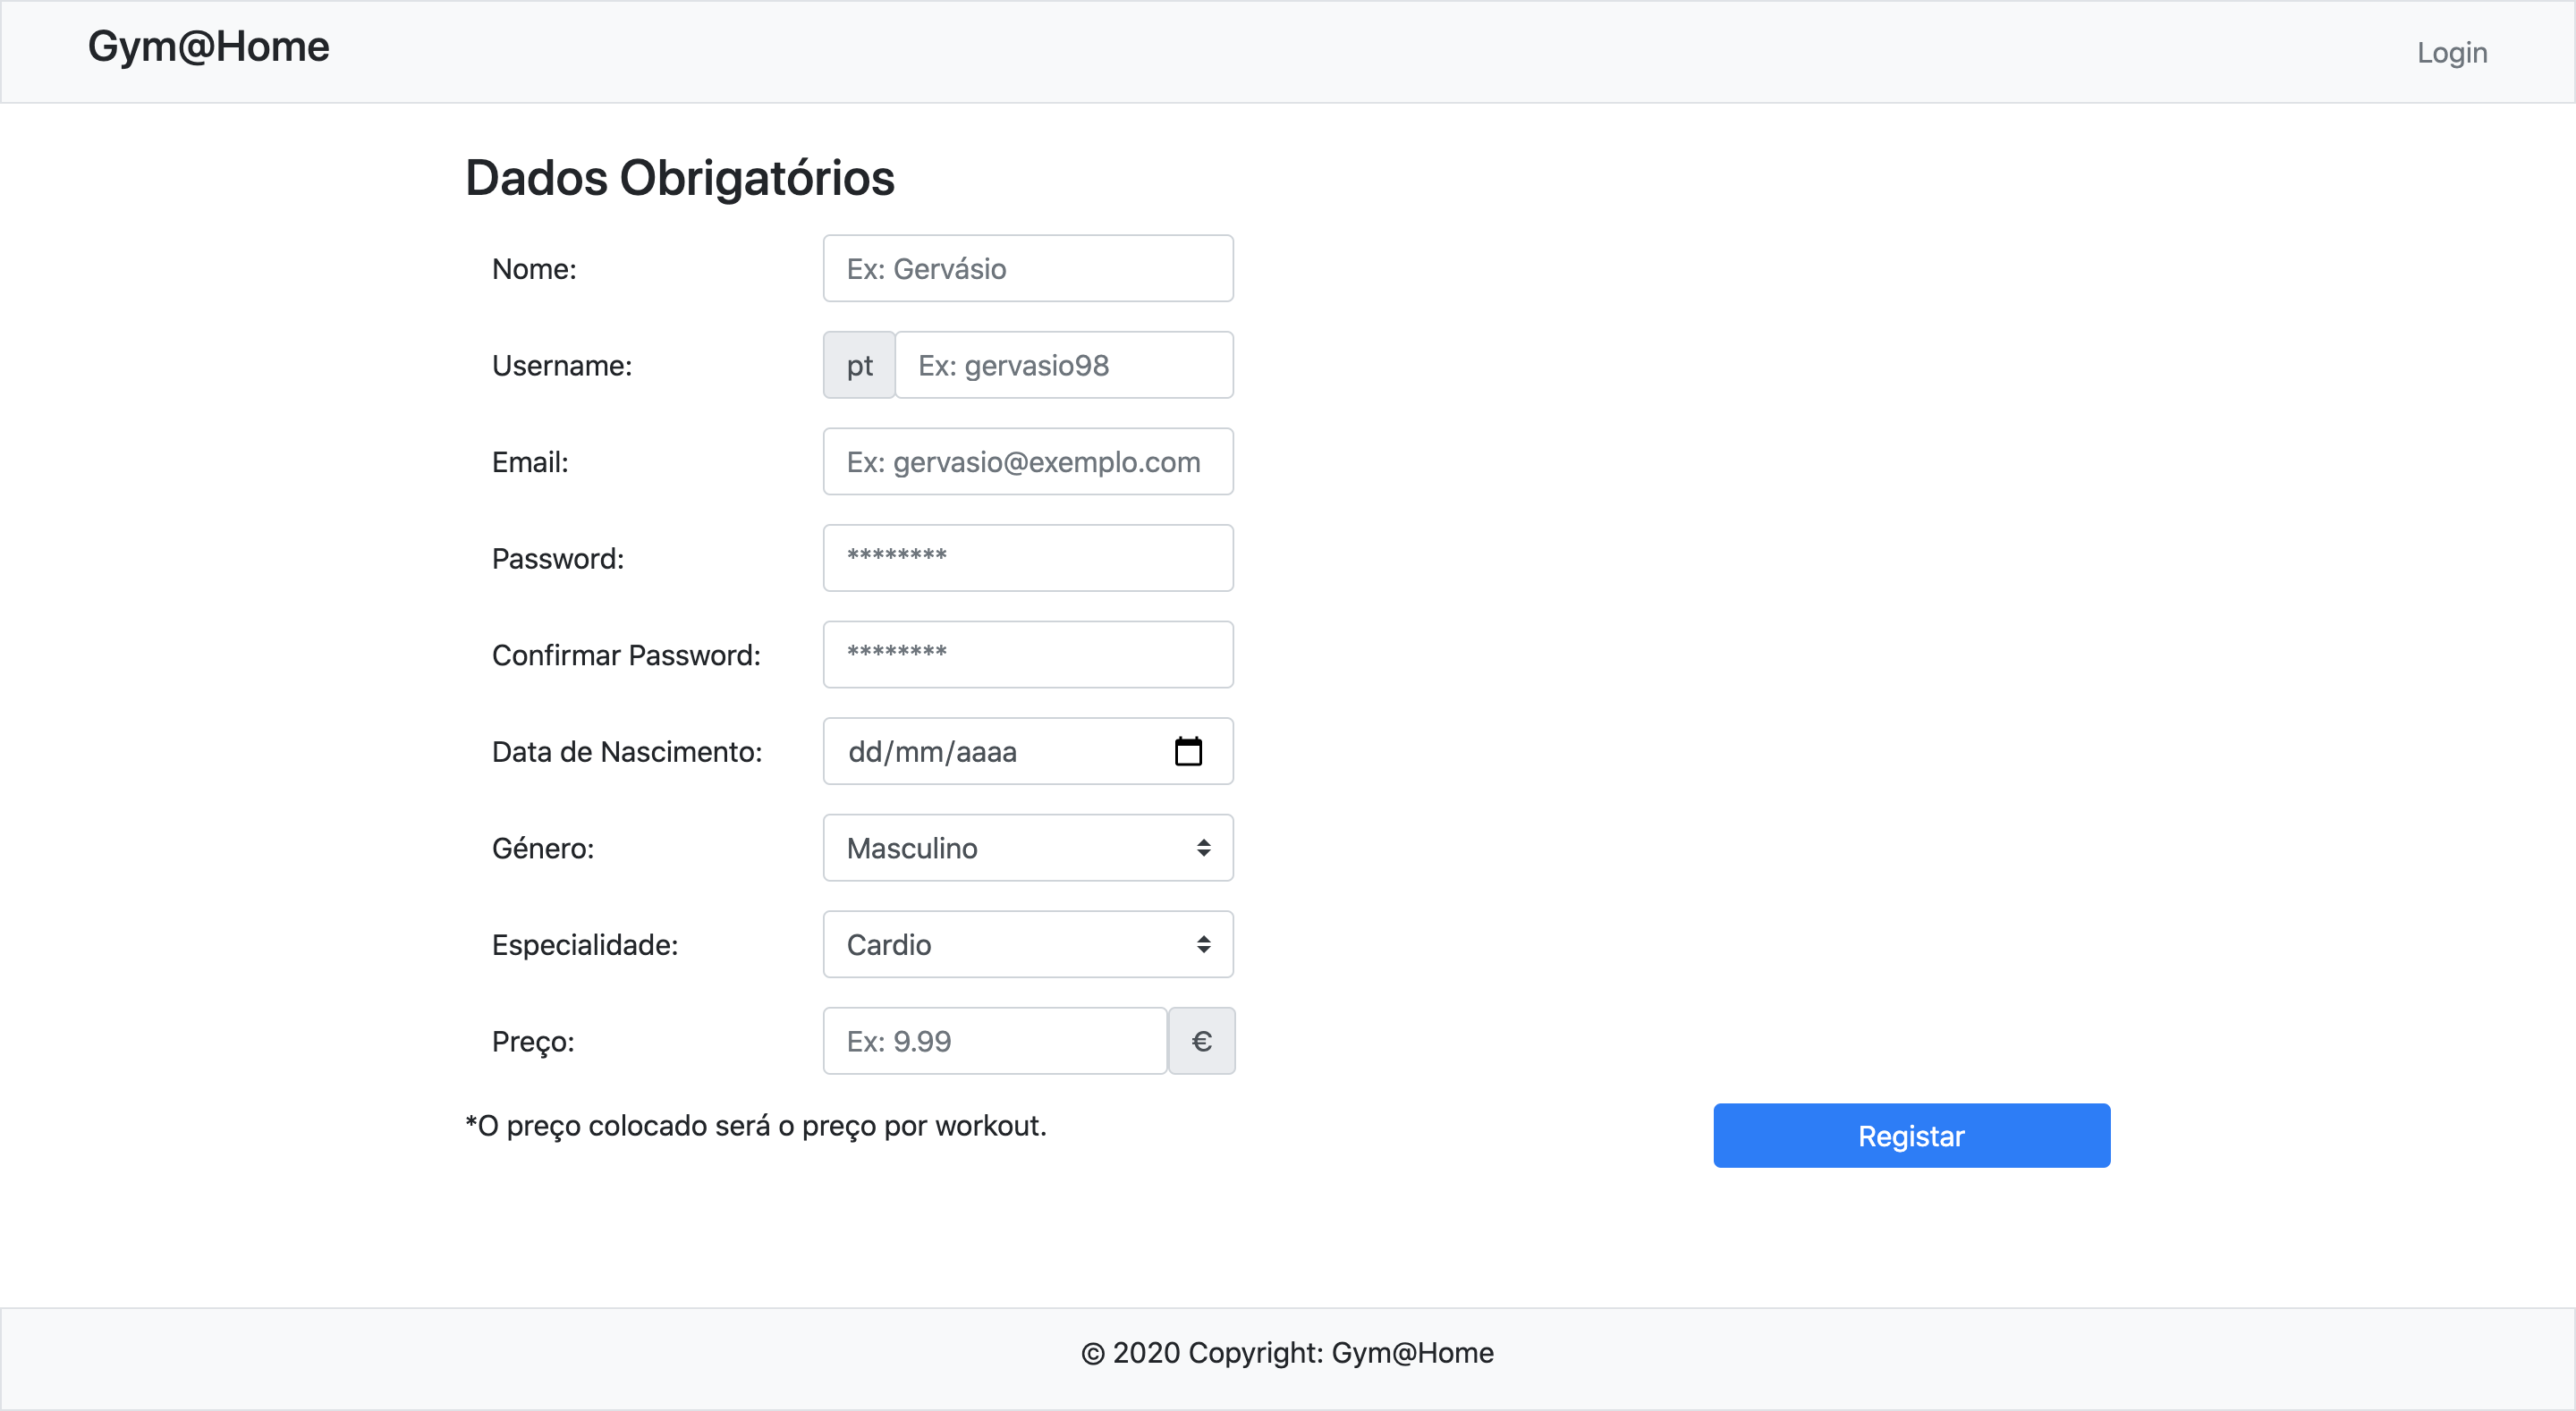
\includegraphics[scale=0.25]{images/interfaces/pt_register.png}
    \caption{Interface Registar PT.}
    \label{fig:interfaceregistarpt}
\end{figure}

\subsubsection{Princípios de Usabilidade}
\begin{itemize}
    \item \textbf{Familiarity} e \textbf{Consistency}: Colocar a "Data de Nascimento" é feito através de um calendário, pelo que o PT como ser humano está mais familiarizado a utilizar.
\end{itemize}

\subsubsection{Heurísticas de Normam}
\begin{itemize}
    \item \textbf{Error prevention}: Todos os inputs numéricos aceitam apenas números, o "Género" e "Especialidade" apenas permite os valores dos dropdowns, a "Data de Nascimento" apenas permite datas seleccionadas pelo calendário e o "Email" apenas aceita um email (tem de conter o @).
    \item \textbf{Consistency and standards}: tal como foi dito anteriormente, segue os princípios de \textbf{Familiarity} e \textbf{Consistency}, pelo que significa que também segue esta heurística relacionada com \textbf{padrões}.
    \item \textbf{Flexibility and efficiency of use}: visto que após ser feito o registo, faz-se o login automático, sendo mais \textbf{eficiente} para o cliente.
\end{itemize}

\subsection{PT consulta/edita o próprio perfil}
\label{subsec:perfilptbypt}

\subsubsection{Descrição}
\hspace{5mm} Do mesmo modo que o Cliente o PT pode visualizar e editar o seu perfil através desta mockup. Também nesta interface final, o botão de "Salvar Alterações" foi deslocado para o cimo da página para facilitar a sua visualização em ecrãs mais pequenos.

\begin{figure}[H]
    \centering
    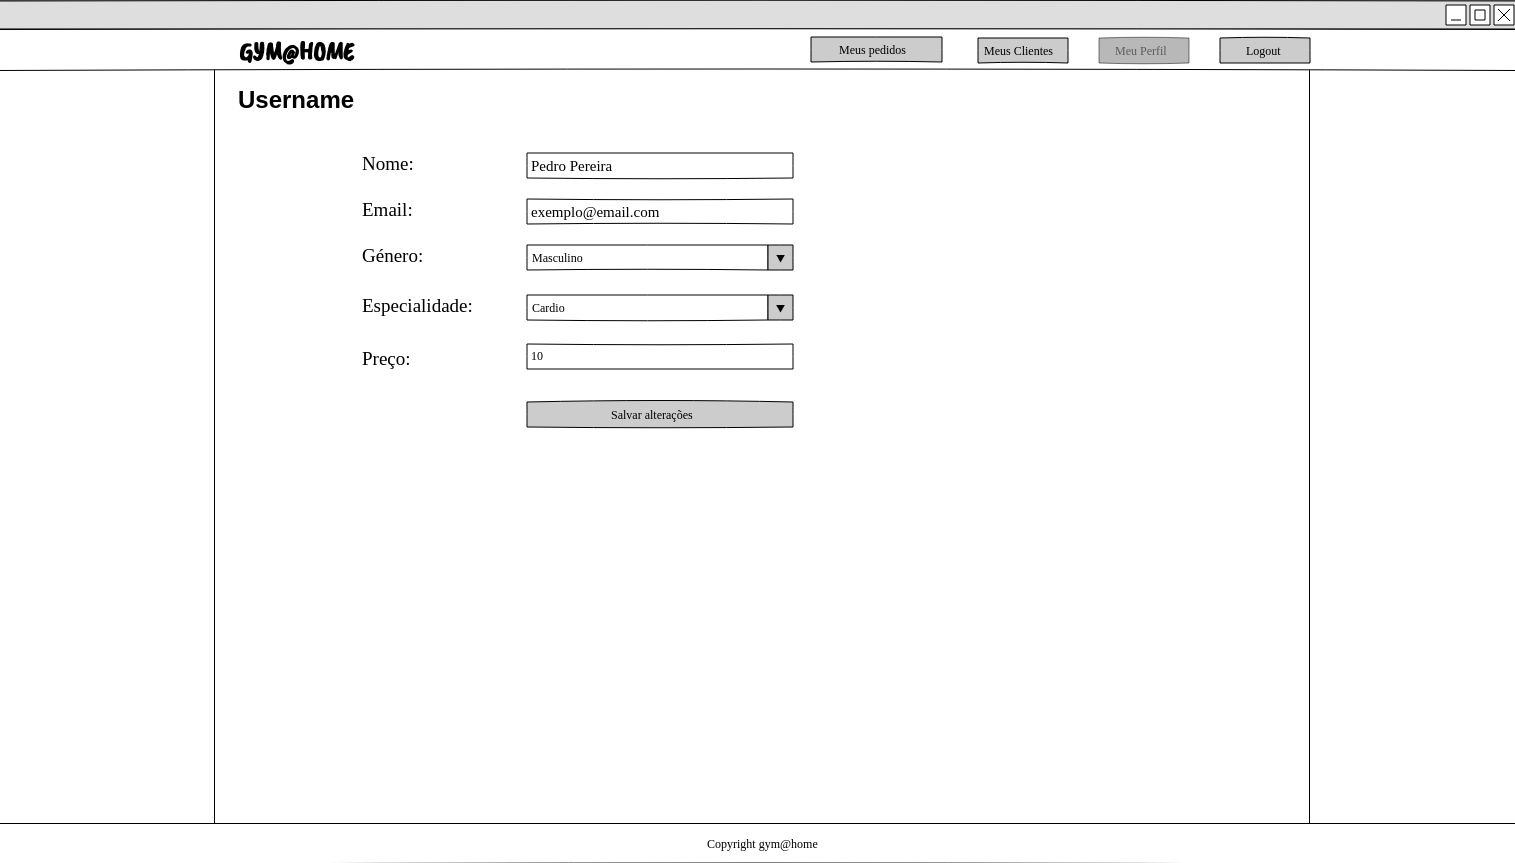
\includegraphics[scale=0.25]{images/mockups/pt_meu_perfil.png}
    \caption{Mockup Perfil PT visto pelo próprio.}
    \label{fig:mockupperfilptbypt}
\end{figure}

\begin{figure}[H]
    \centering
    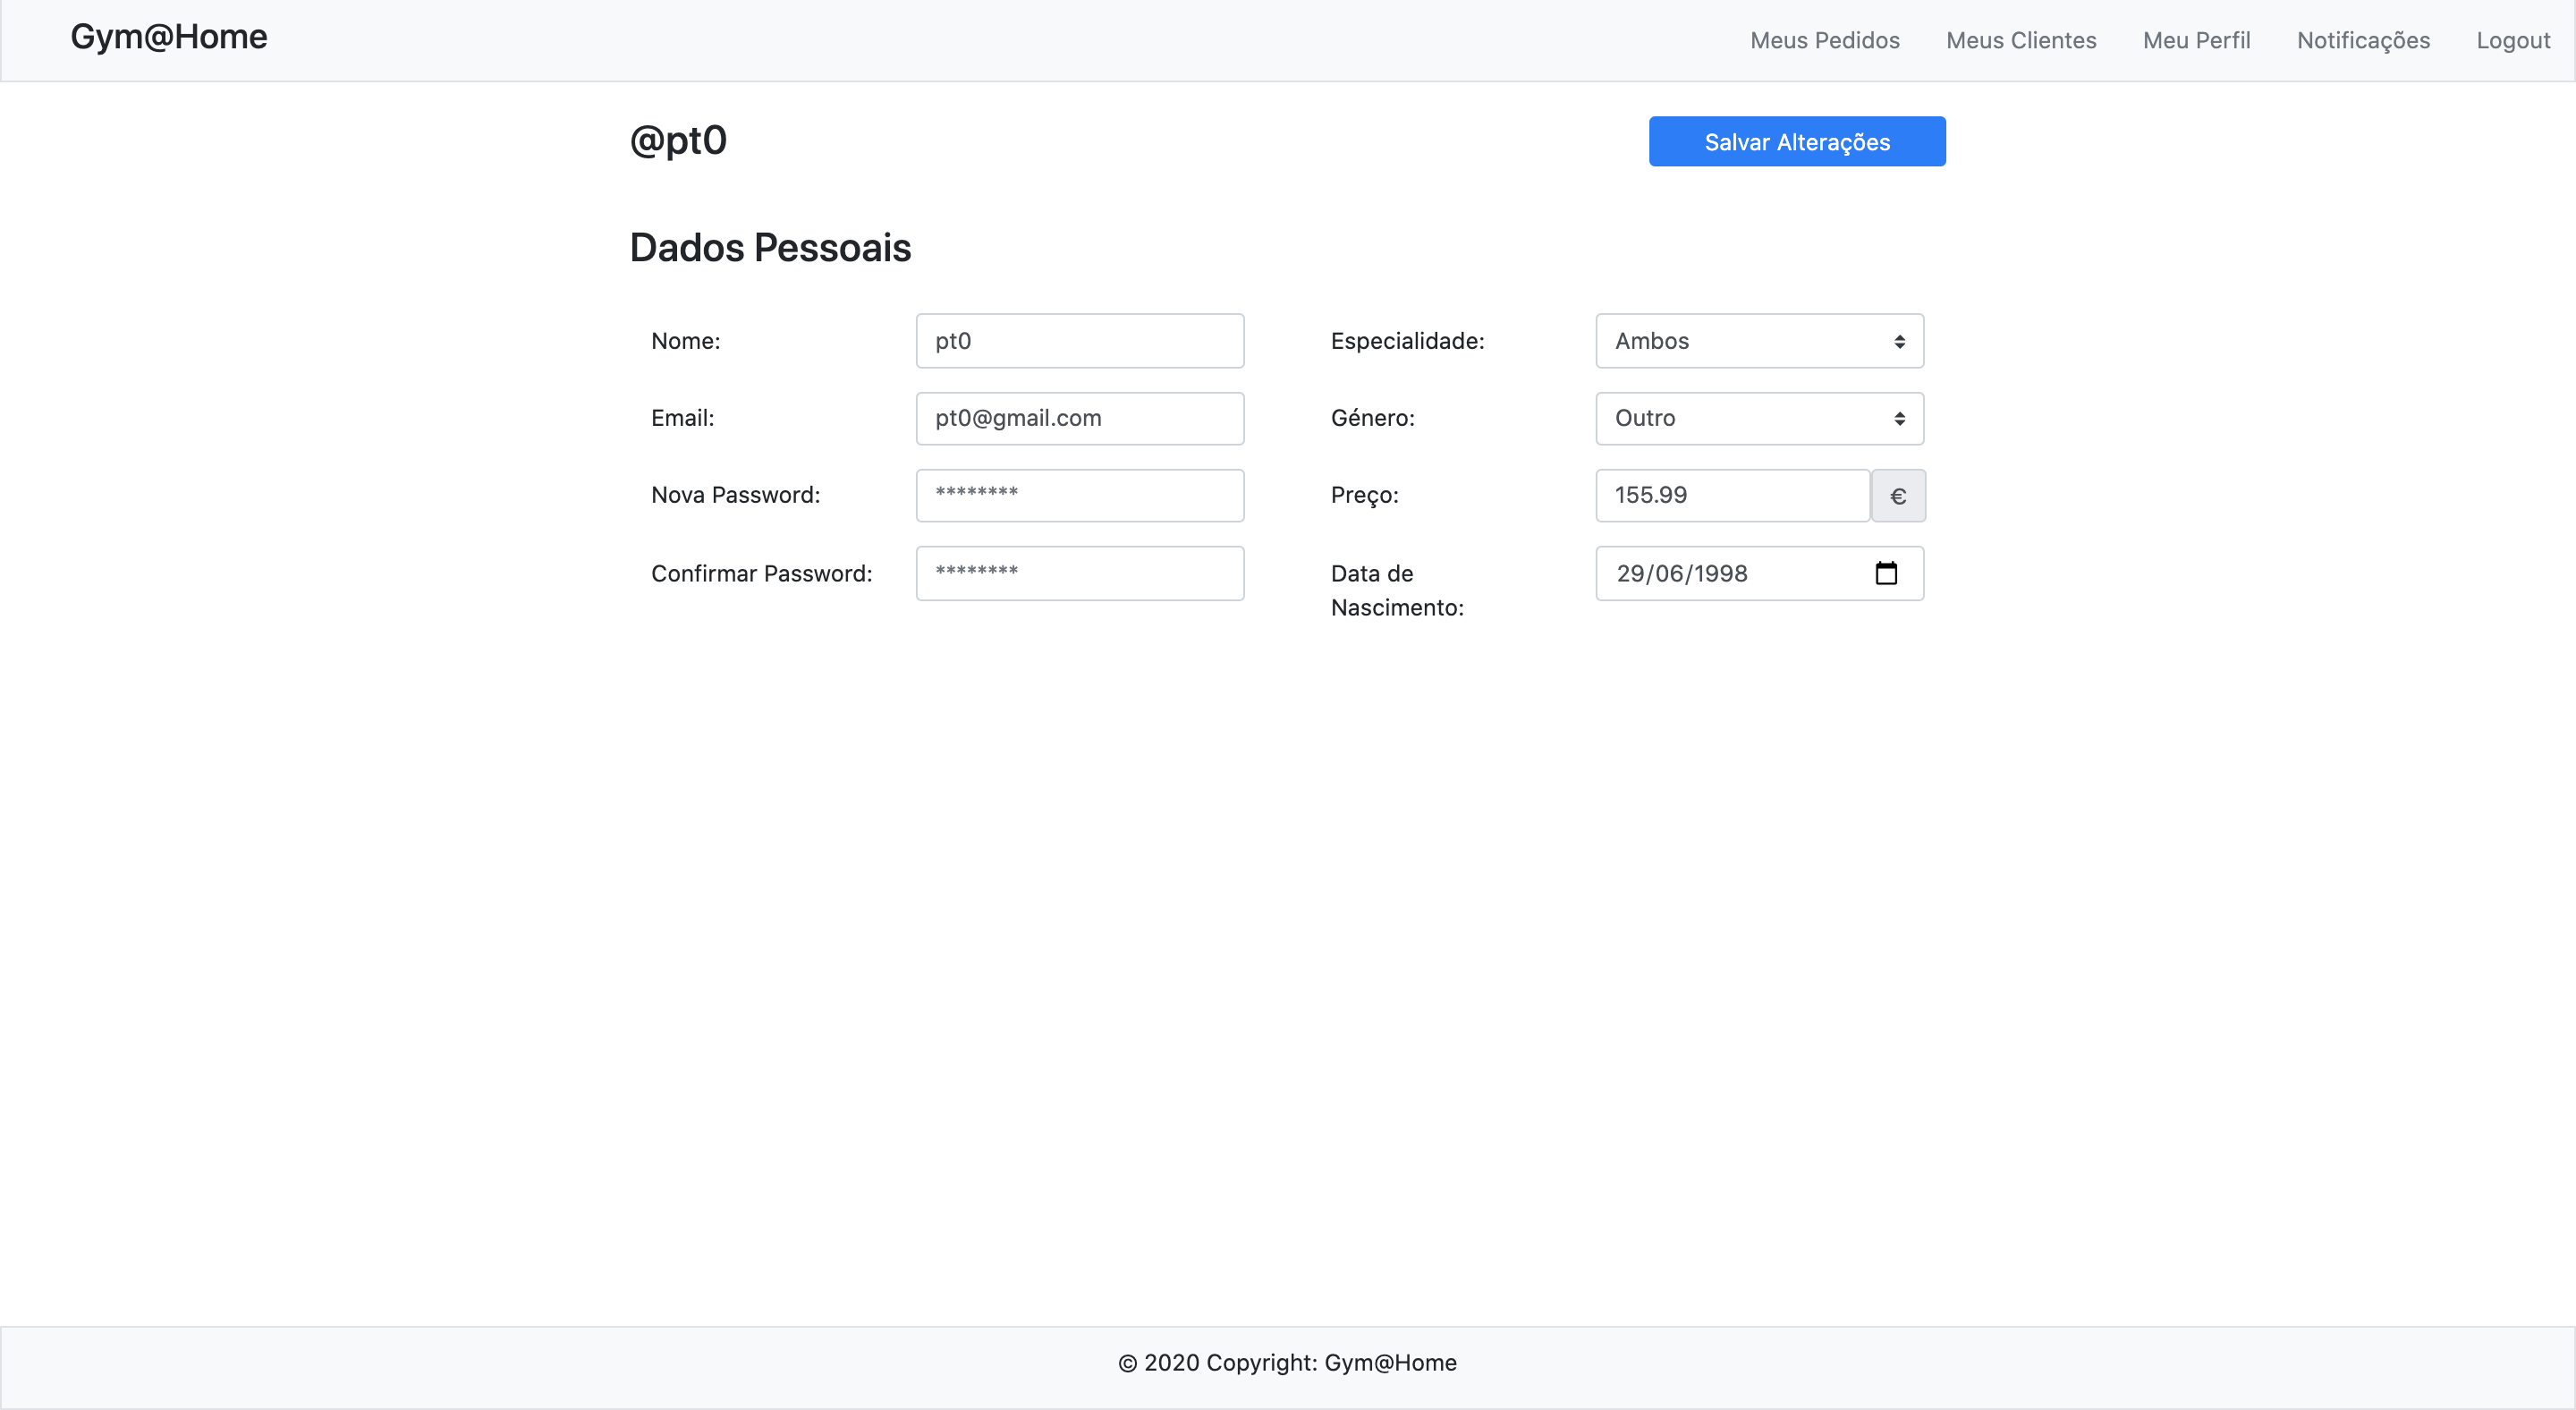
\includegraphics[scale=0.25]{images/interfaces/pt_perfil.png}
    \caption{Interface Perfil PT visto pelo próprio.}
    \label{fig:interfaceperfilptbypt}
\end{figure}

\subsubsection{Princípios de usabilidade}
\begin{itemize}
   \item \textbf{Substitutivity}: Os inputs da interface onde o PT pode alterar os valores são também outputs. Sempre que o PT alterar dados estes são guardados na BD e novamente carregados para os outputs que o PT tinha utilizado como input.
    
    \item \textbf{Observability}: O botão "Salvar Alterações" está no cimo da página para o PT o conseguir observar mal carregue a página.
    
    \item \textbf{Familiarity}: Colocar a "Data de Nascimento" é feito através de um calendário, pelo que o PT como ser humano está mais familiarizado a utilizar.
\end{itemize}

\subsubsection{Heurísticas de Normam}
\begin{itemize}
    \item \textbf{Error prevention}: Todos os inputs numéricos aceitam apenas números, o "Género" e "Especialidade" apenas permite os valores dos dropdowns, a "Data de Nascimento" apenas permite datas seleccionadas pelo calendário e o "Email" apenas aceita um email (tem de conter o @).
    \item \textbf{Flexibility and efficiency of use}: tal como diz respeito ao principio \textbf{Substitutivity}, usar o mesmo componente quer para visualizar, quer para editar o perfil, torna a interface mais eficiente para o PT.
\end{itemize}

\subsection{Consulta do perfil do Cliente pelo PT}
\label{subsec:perfilclientbypt}

\subsubsection{Descrição}
\hspace{5mm} Com o objectivo de facilitar o acesso rápido às informações do Cliente sem ter que ir para uma nova página e voltar, colocou-se um botão/atalho, que mostra os mesmos num pop-up, sendo isto possível e consistente em diversas interfaces, sendo que no lado do PT será no "Meus Clientes" e "Meus Pedidos de Clientes". 

\hspace{5mm} Assim reduziu-se a quantidade de cliques necessários para aceder aos dados, desta forma, acha-se que foi um boa melhoria, principalmente no ponto de vista do PT que fará esta acção repetitivamente, tornando assim a utilização da aplicação mais eficiente. 

\hspace{5mm} A alteração para pop-up, torna-se bastante diferente do protótipo, no entanto, as alterações na opinião da equipa foram para melhorar.

\begin{figure}[H]
    \centering
    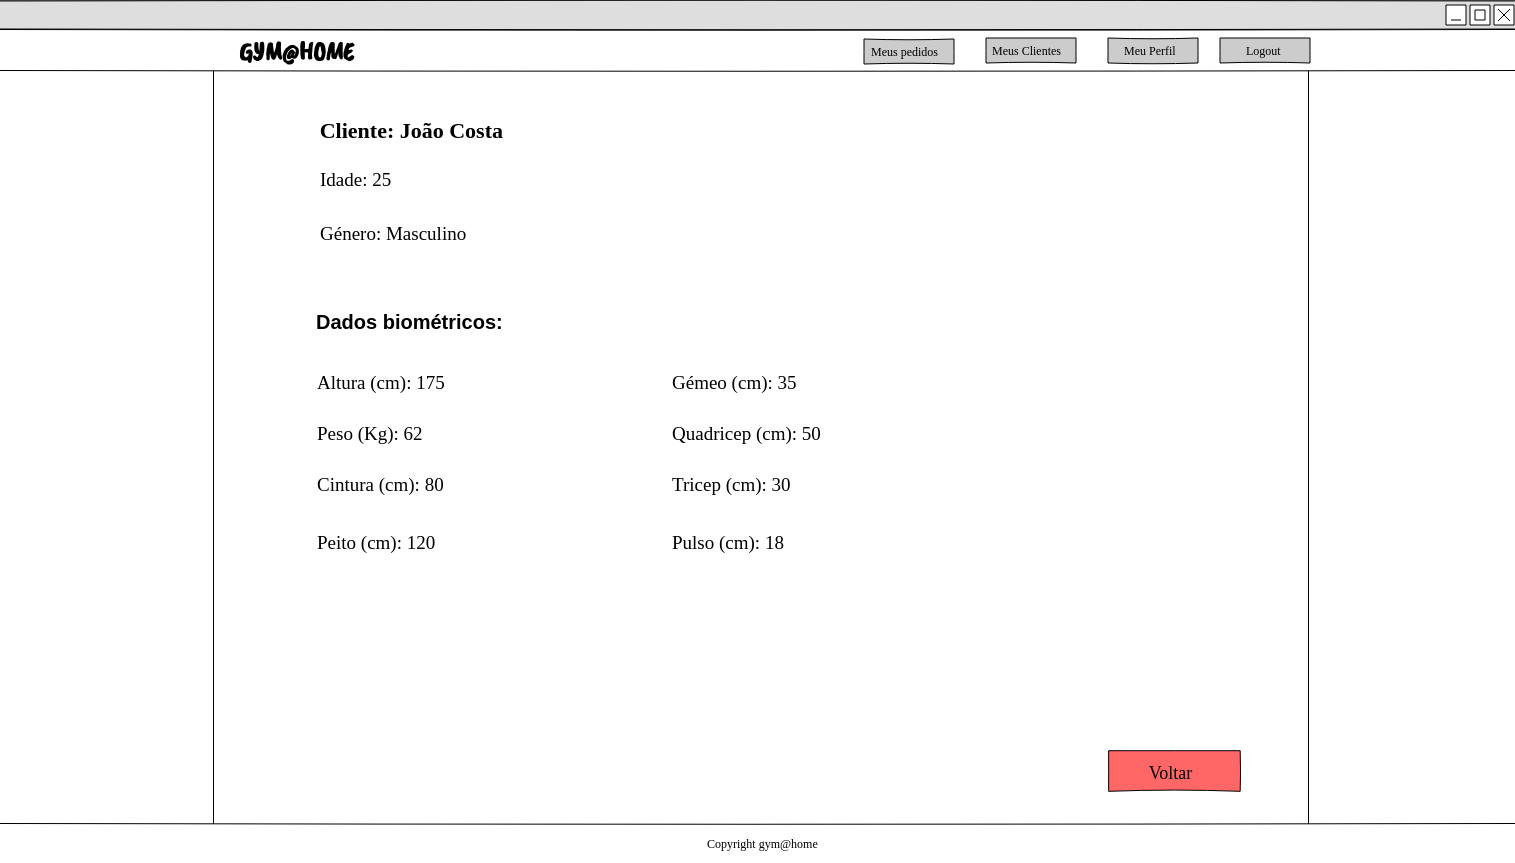
\includegraphics[scale=0.25]{images/mockups/pt_dados_cliente.png}
    \caption{Mockup Perfil Cliente visto pelo PT.}
    \label{fig:mockupperfilclientebypt}
\end{figure}

\begin{figure}[H]
    \centering
    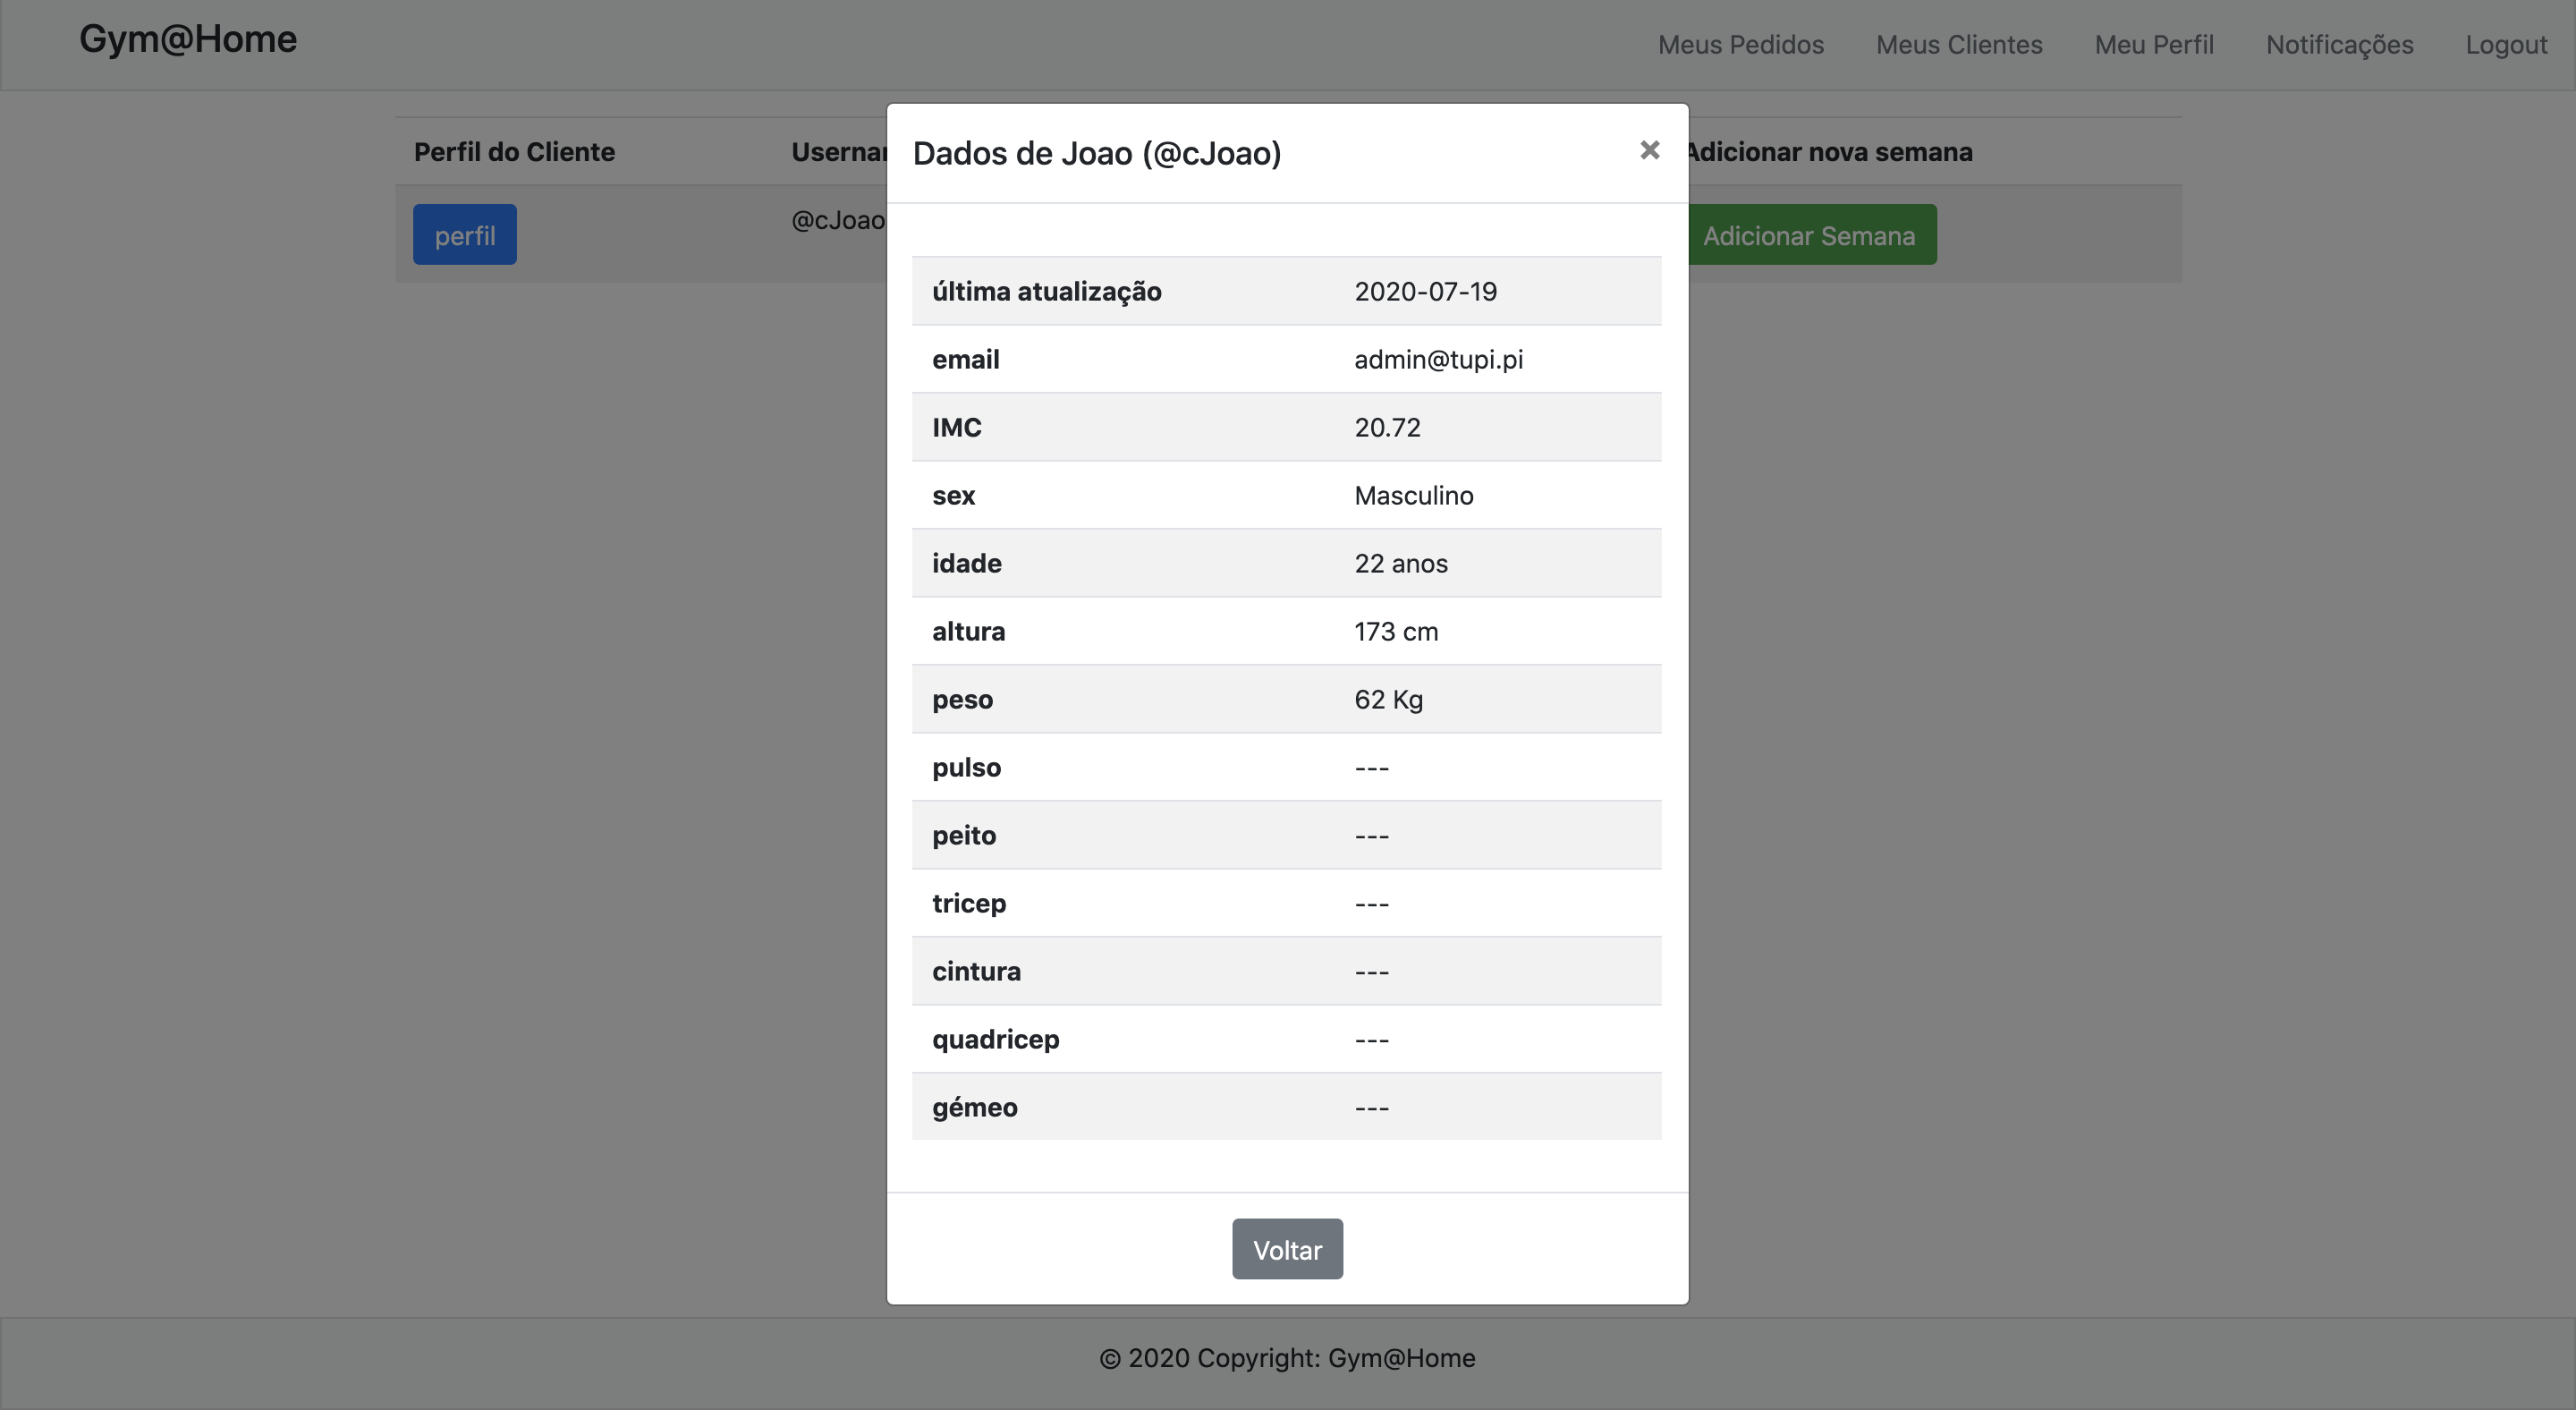
\includegraphics[scale=0.25]{images/interfaces/pt_perfil_cliente.png}
    \caption{Interface Perfil Cliente visto pelo PT.}
    \label{fig:interfaceperfilclientebypt}
\end{figure}

\subsubsection{Princípios de usabilidade}
\begin{itemize}
    \item \textbf{Consistency}: na medida em que, mantêm-se sempre a mesma forma de apresentar o perfil (pop-up) nas várias views que necessitem dessa informação. Pode-se também considerar consistente devido ao facto de a apresentação do perfil do PT ter a mesma estrutura mas com campos diferentes.
    
    \item \textbf{Flexibility and efficiency of use}: o botão "perfil", que mostra as informações do Cliente torna esse processo de consulta mais \textbf{eficiente}, como uma espécie de atalho.
\end{itemize}

\subsubsection{Heurísticas de Normam}
\begin{itemize}
    \item \textbf{Consistency and Standards}: devido à consistência da mesma forma de apresentação pelas várias mockups que necessitam de aceder à informação do cliente.
    \item \textbf{Flexibility and efficiency of use}: o botão de "perfil" presente em algumas interfaces que necessitam de consultar os dados do cliente, torna esse processo mais eficiente para o utilizador, neste caso para o PT. Principalmente para este utilizador, que poderá lidar com muitos pedidos de plano, e para tal precisará de consultar os dados dos clientes, e com apenas um clique consegue fazê-lo.
\end{itemize}

\subsection{Pedidos recebidos pelo PT}
\label{subsec:pedidosclientes}

\subsubsection{Descrição}
\hspace{5mm} Inicialmente importa referir que esta foi uma das interfaces que mudou drasticamente em relação ao prototipo, pois achou-se que não fazia sentido. Primeiramente a tabela lateral apenas tinha o nome do cliente, o que não é nada informativo para o PT. Depois, o PT tinha que clicar na tabela para ver os dados do formulário de cada cliente, o que não é \textbf{eficiente} para o mesmo. Do mesmo modo como já foi referido, o botão para consultar o perfil na página do cliente não é de todo a forma mais eficiente. 

\hspace{5mm}A solução para tornar esta interface mais eficiente, foi em listar os pedidos, bem como os dados mais importantes referentes ao pedido (campos do formulário), permitindo facilmente ao PT ver a informação de cada pedido sem necessitar de clicar em cada cliente. Isto permite por exemplo excluir alguns pedidos apenas olhando para estes dados da tabela. No entanto, consultar os dados biométricos 
é importante em certas situações para se decidir se aceita ou rejeita o pedido. Dessa forma, e como em outras views onde se necessita de consultar dados de perfil, colou-se um botão em cada pedido para aparecer um pop up com a informação do cliente. Como por vezes o PT pode decidir no momento em que consulta esses dados se vai aceitar ou rejeitar, logo, propaga-se os botões de aceitar ou rejeitar para esse pop-up.

\hspace{5mm} Após aceitar um pedido, será redireccionado para a interface "Criar uma semana do plano", caso rejeite, fica na mesma interface e o pedido é removido da tabela.

\begin{figure}[H]
    \centering
    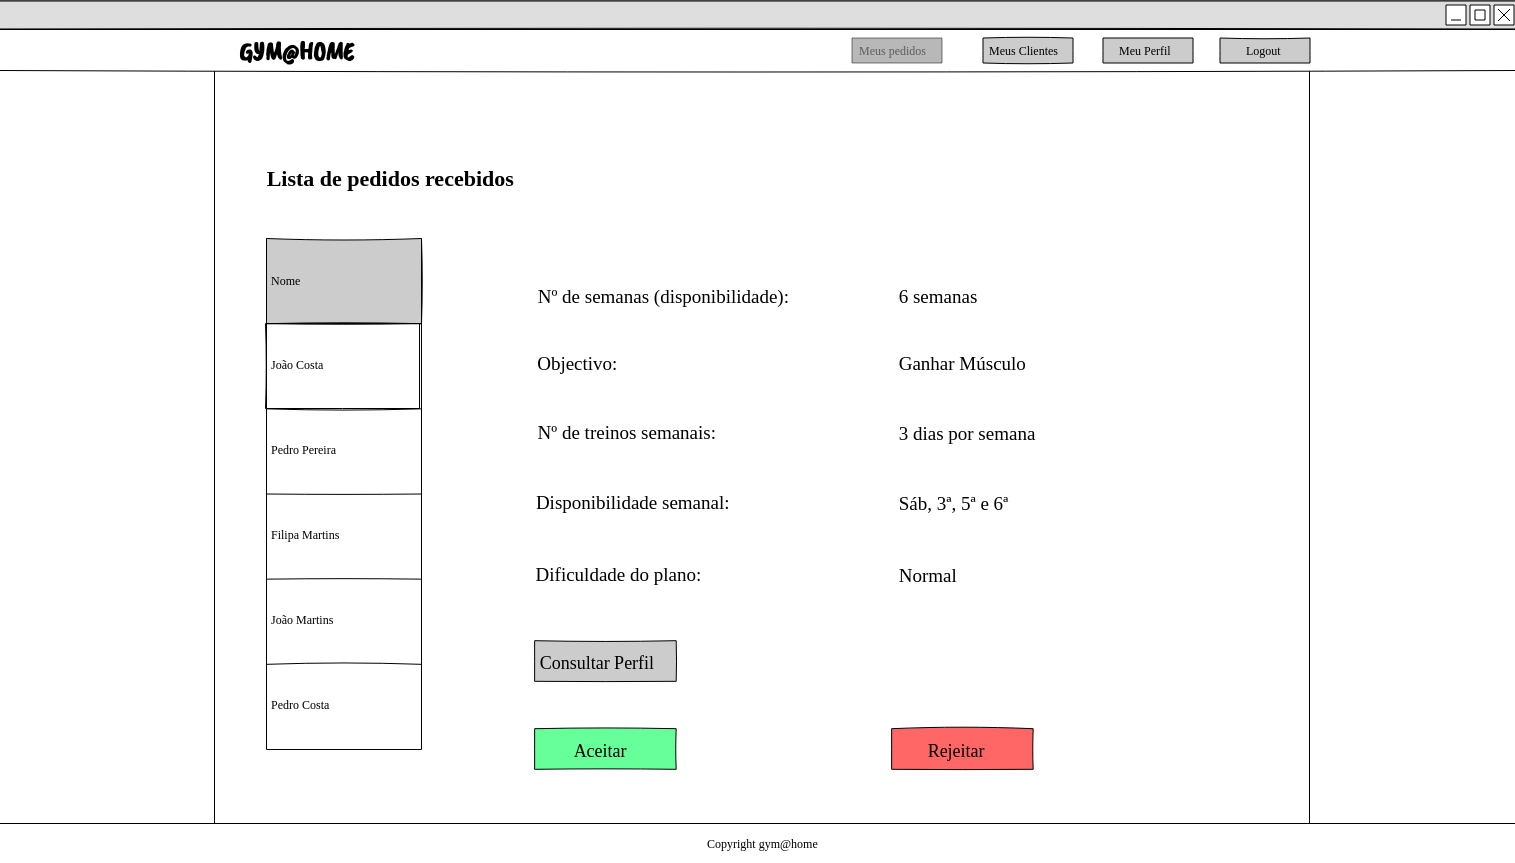
\includegraphics[scale=0.25]{images/mockups/pt_meus_pedidos_joo_costa.png}
    \caption{Mockup Pedidos Clientes.}
    \label{fig:mockuppedidosclientes}
\end{figure}

\begin{figure}[H]
    \centering
    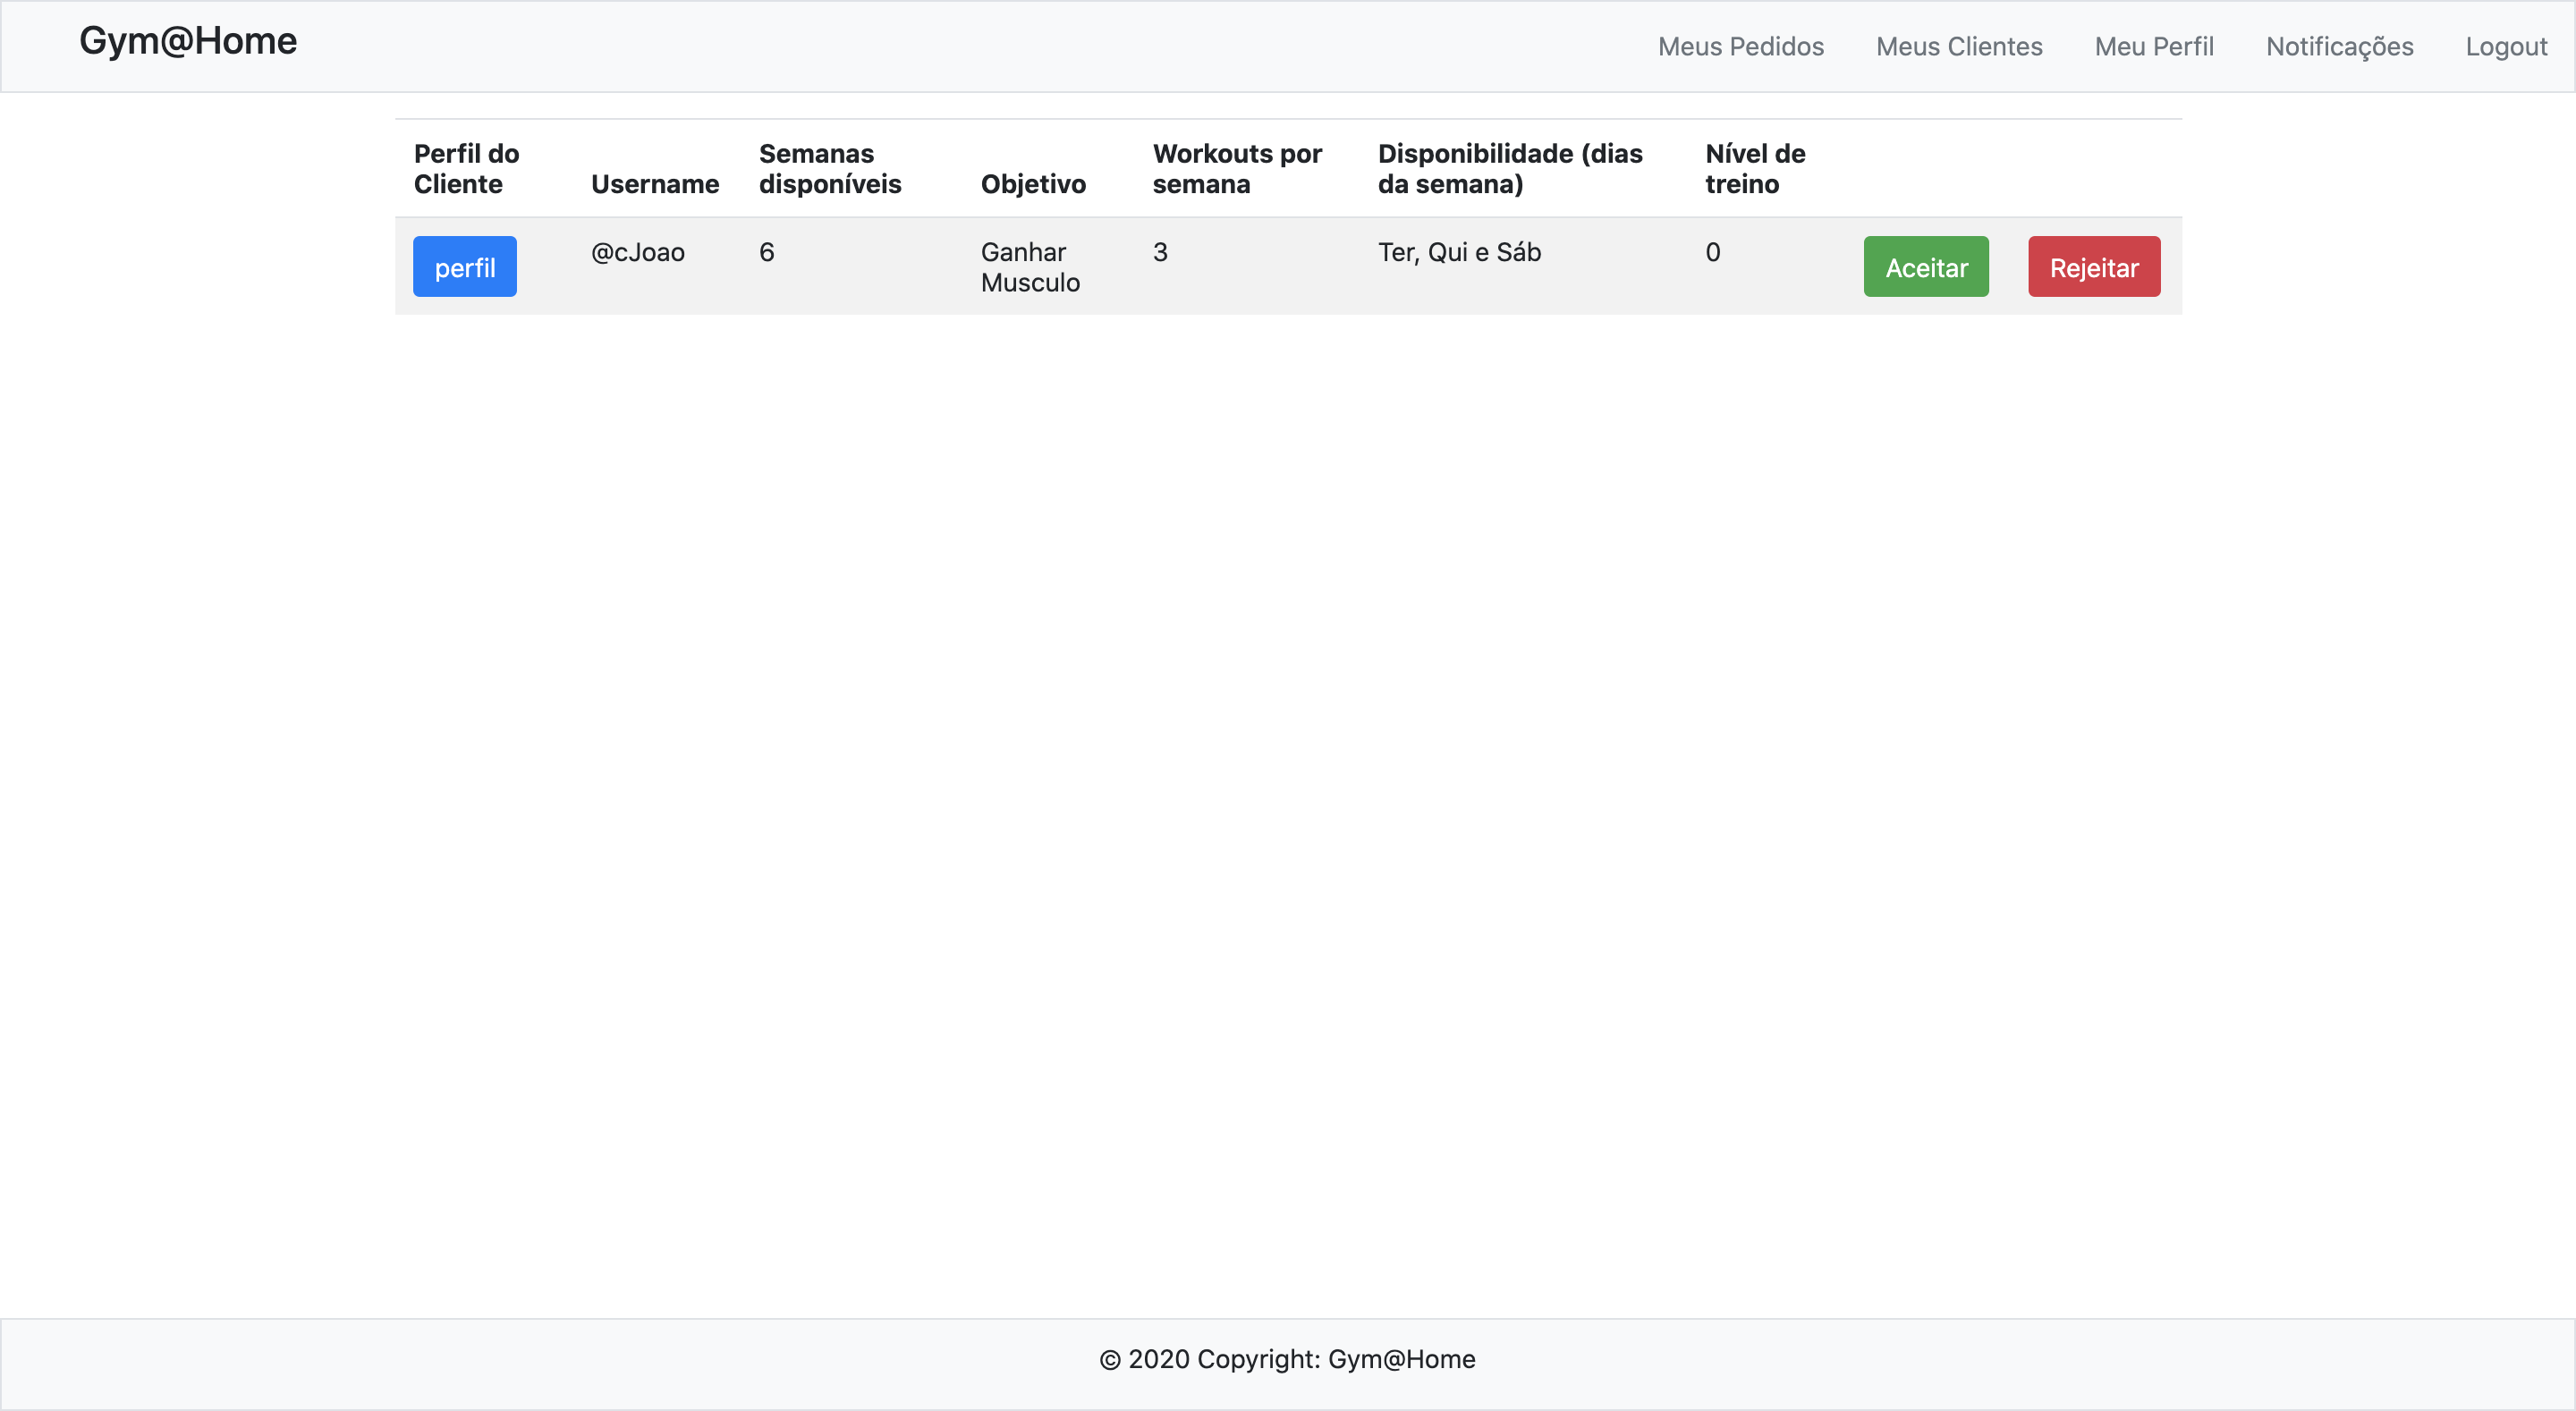
\includegraphics[scale=0.25]{images/interfaces/pt_meus_pedidos.png}
    \caption{Interface Pedidos Clientes.}
    \label{fig:interfacepedidosclientes}
\end{figure}

\subsubsection{Princípios de usabilidade}
\begin{itemize}
    \item \textbf{Synthesizability}: uma das acções possíveis nesta interface consiste em consultar o perfil do Cliente, pelo que após clicar no botão "perfil", aparece um pop-up com as informações do mesmo, ou seja, o PT consegue perceber o efeito das suas acções. Por outro lado, o botão aceitar, redireciona para a página "Criar semana do plano", logo, da mesma forma, o PT, também percebe o efeito da sua ação. Por fim, o rejeitar, marca o pedido como rejeitado, e o mesmo não aparecerá na tabela no próximo refresh, mostrando ao PT o efeito de ter rejeitado.
    \item \textbf{Generalizability} e \textbf{Consistency}: tal como já foi dito, o Cliente também contem uma interface para ver os pedidos enviados pelo o mesmo, que a nível de estrutura pode-se considerar bastante semelhante a este, difere apenas no conteúdos de algumas colunas, pelo que se pode considerar que se trata de uma interface genérica/consistente no sistema. 
    \item \textbf{Observability}: esta interface pode aumentar bastante o número de linhas da tabela, no entanto cada linha tem os botões para as acções desse pedido, o que significa que se houvesse uma tabela gigante, as acções possíveis estariam lá, não necessitando de subir a página ou outra forma para encontrar os botões. No entanto o grupo reconhece que aqui também seria um bom candidato a paginação, não sendo possível implementar face à falta de tempo, mas será uma boa actualização no futuro.
\end{itemize}

\subsubsection{Heurísticas de Normam}
\begin{itemize}
    \item \textbf{Recognition rather than recall}: o PT não precisa de memorizar as informações dos formulários no momento em que aceita, pois esses dados são enviados para a interface "Criar Semana do Plano".
    \item \textbf{Flexibility and efficiency of use}: o botão "perfil", que mostra as informações do Cliente torna esse processo de consulta mais \textbf{eficiente}, como uma espécie de atalho.
    
\end{itemize}

\subsection{Clientes do PT}
\label{subsec:clientes}
\subsubsection{Descrição}
\hspace{5mm} A interface permite ao PT ter acesso rápido a todos os seus Clientes, que tem actualmente, com a finalidade de ver o Plano de cada um, o perfil ou adicionar uma nova semana aos planos dos mesmos.

\hspace{5mm} Em cada linha da tabela, aparecem os botões referentes às funcionalidades referidas acima associados a cada cliente.

\begin{figure}[H]
    \centering
    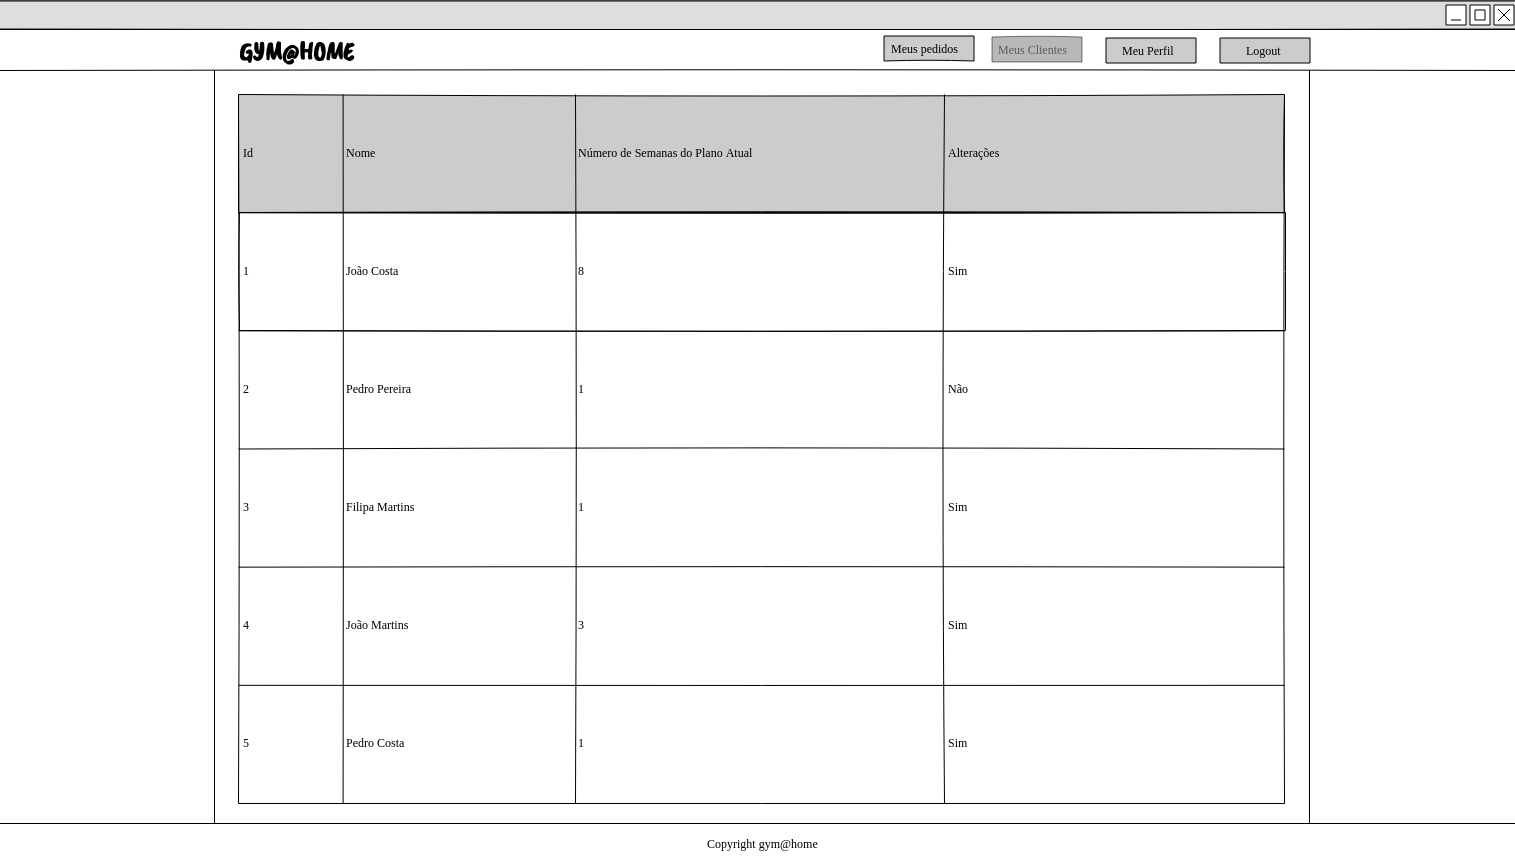
\includegraphics[scale=0.25]{images/mockups/personal_trainer_listar_clientes.png}
    \caption{Mockup Clientes do PT.}
    \label{fig:mockupclientes}
\end{figure}

\begin{figure}[H]
    \centering
    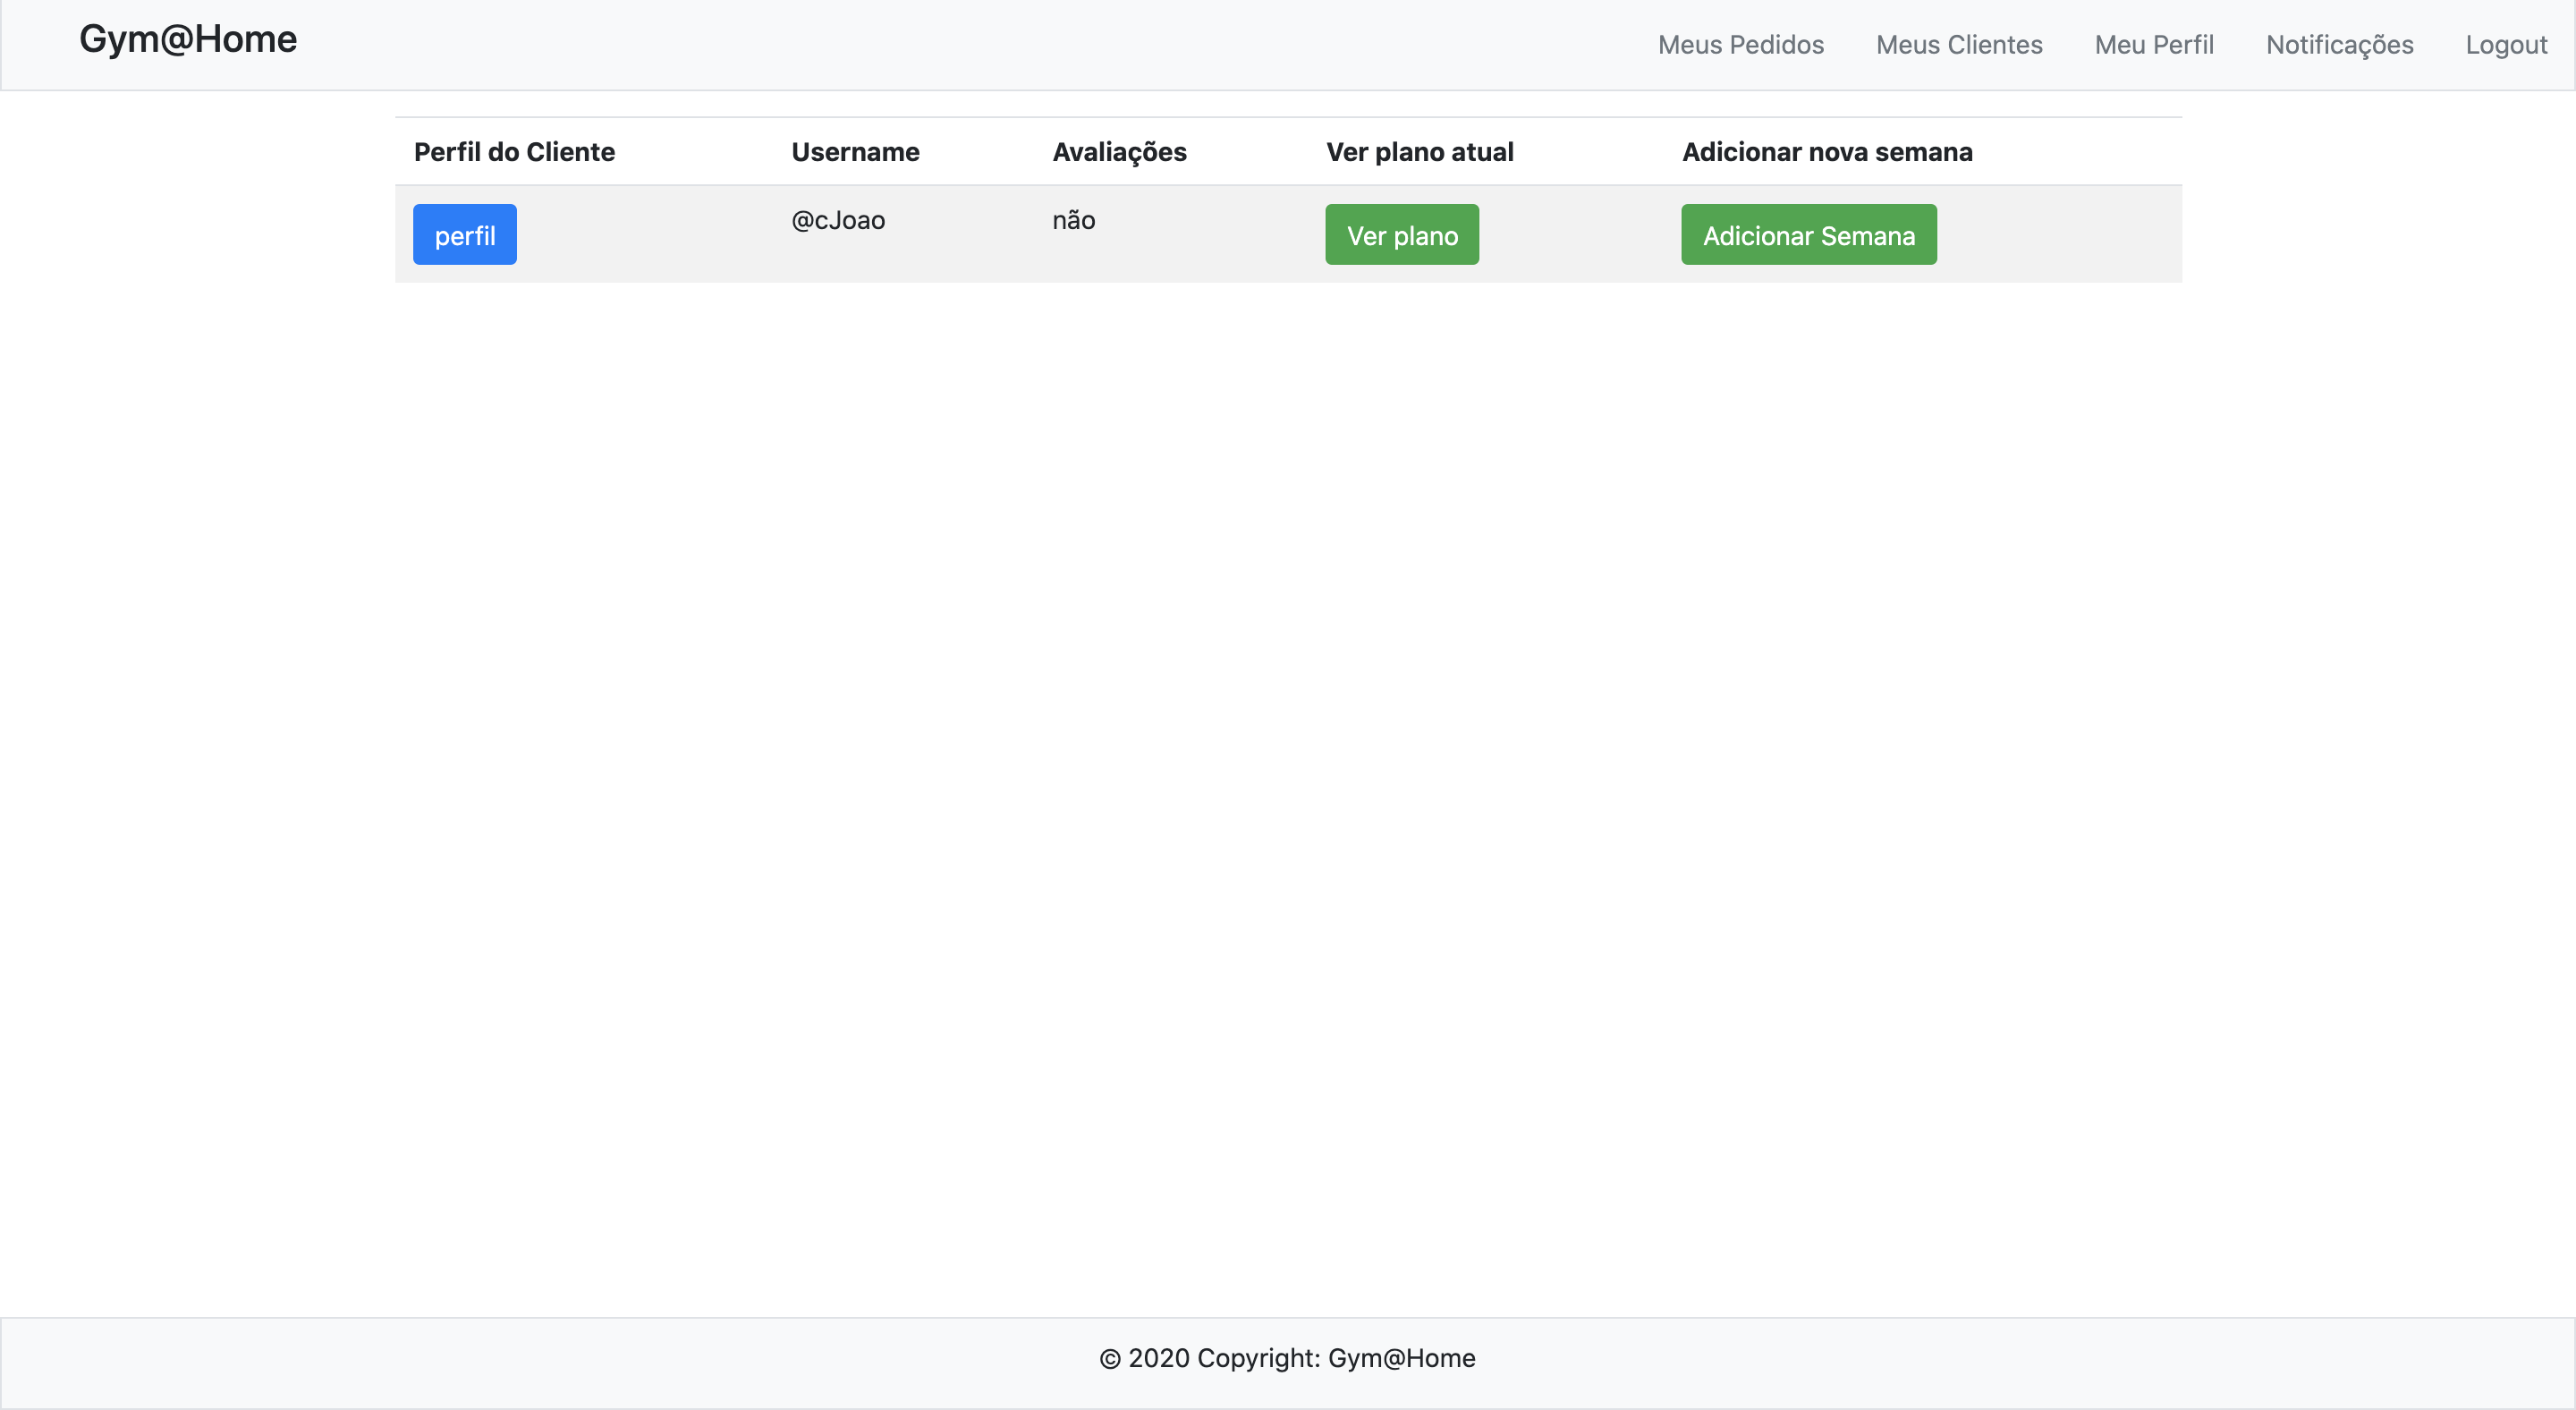
\includegraphics[scale=0.25]{images/interfaces/pt_meus_clientes.png}
    \caption{Interface Clientes do PT.}
    \label{fig:interfaceclientes}
\end{figure}

\subsubsection{Princípios de usabilidade}
\begin{itemize}
    \item \textbf{Synthesizability}: uma das acções possíveis nesta interface consiste em consultar o perfil do Cliente, pelo que após clicar no botão "perfil", aparece um pop-up com as informações do mesmo, ou seja, o PT consegue perceber o efeito das suas acções. Por outro lado, o botão ver plano, redirecciona para a página "Consultar Plano", logo, da mesma forma, o PT, também percebe o efeito da sua acção. Por fim, o adicionar semana, redirecciona para a página "Adicionar Semana", pelo que o PT percebe o efeito da sua acção.
    \item \textbf{Observability}: esta interface pode aumentar bastante o número de linhas da tabela, no entanto cada linha tem os botões para as acções desse cliente, o que significa que se houvesse uma tabela gigante, as acções possíveis estariam lá, não necessitando de subir a página ou outra forma para encontrar os botões. No entanto, o grupo reconhece que aqui também seria um bom candidato a paginação, não sendo possível implementar face à falta de tempo, mas será uma boa actualização no futuro.
\end{itemize}

\subsubsection{Heurísticas de Normam}
\begin{itemize}
    \item \textbf{Recognition rather than recall}: o PT não precisa de memorizar as informações do cliente no momento em que cria uma nova semana para o plano do mesmo , pois esses dados são enviados para a interface "Criar Semana do Plano".
    \item \textbf{Flexibility and efficiency of use}: o botão "perfil", que mostra as informações do Cliente torna esse processo de consulta mais \textbf{eficiente}, como uma espécie de atalho.
    
\end{itemize}

\subsection{Criar Semana}
\label{subsec:criarsemana}
\hspace{5mm} O workout "Criar Semana" foi um dos mockups que teve que ser revisto face à primeira fase de apresentação do projecto, após o conselho da equipa docente de repensar o mesmo, pois estava demasiado complexo, confuso e pouco usável. A equipa decidiu que teria de ser tudo feito numa única página. Dessa forma, Chegou-se ao resultado que se pode ver nas figuras \ref{fig:mockupcriarsemana} e \ref{fig:interfacecriarsemana}.

\hspace{5mm} Primeiramente, importa realçar o preload dos dados do formulário do cliente, importantes para saber criar a semana. À esquerda, tem-se uma tabela, com os workouts criados, sendo que inicialmente estará vazia. Depois tem-se a escolha do nome para o workout, bem como o dia da semana, sendo que este dropDown dos dias, vai automaticamente buscar os dias do formulário e reduzindo-os cada vez que se faz um workout. Por fim, tem-se uma tabela, super dinâmica, que aumenta e diminui de linhas, permitindo ao PT adicionar/remover o número de tarefas que pretender, não sendo um valor fixo.

\hspace{5mm} Importante realçar nesta interface que a semana só é guardada no momento em que clicar no botão guardar semana, caso contrário, tudo que foi criada é descartado. Como se trata de opções impossíveis de reverter, também são difíceis de realizar, pois aparece sempre um pop-up a perguntar se tem a certeza da acção.


\subsubsection{Descrição}
\hspace{5mm} 

\begin{figure}[H]
    \centering
    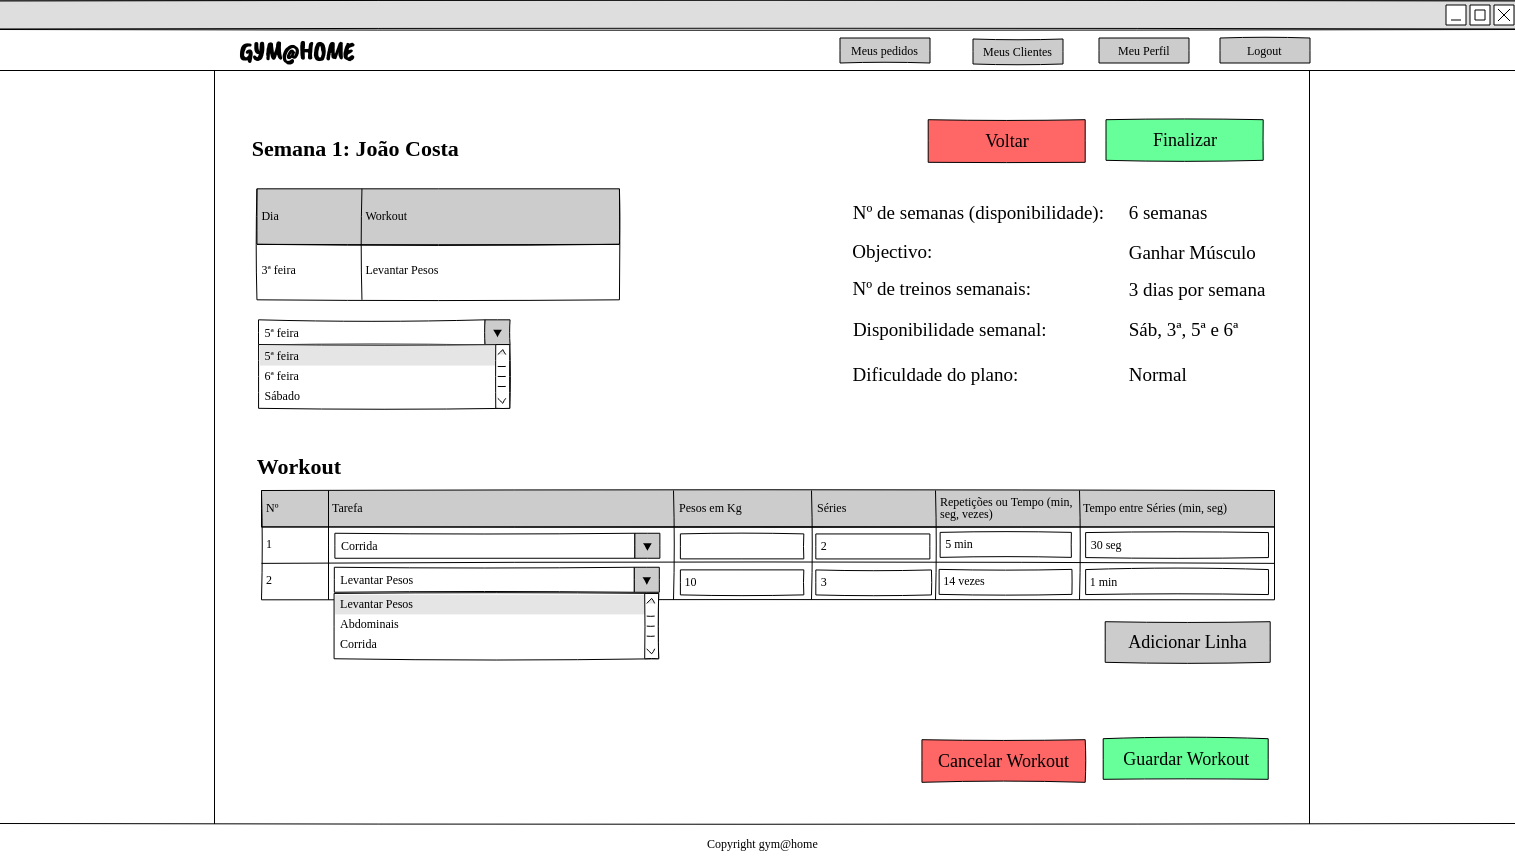
\includegraphics[scale=0.25]{images/mockups/pt_criar_semana.png}
    \caption{Mockup Criar Semana.}
    \label{fig:mockupcriarsemana}
\end{figure}

\begin{figure}[H]
    \centering
    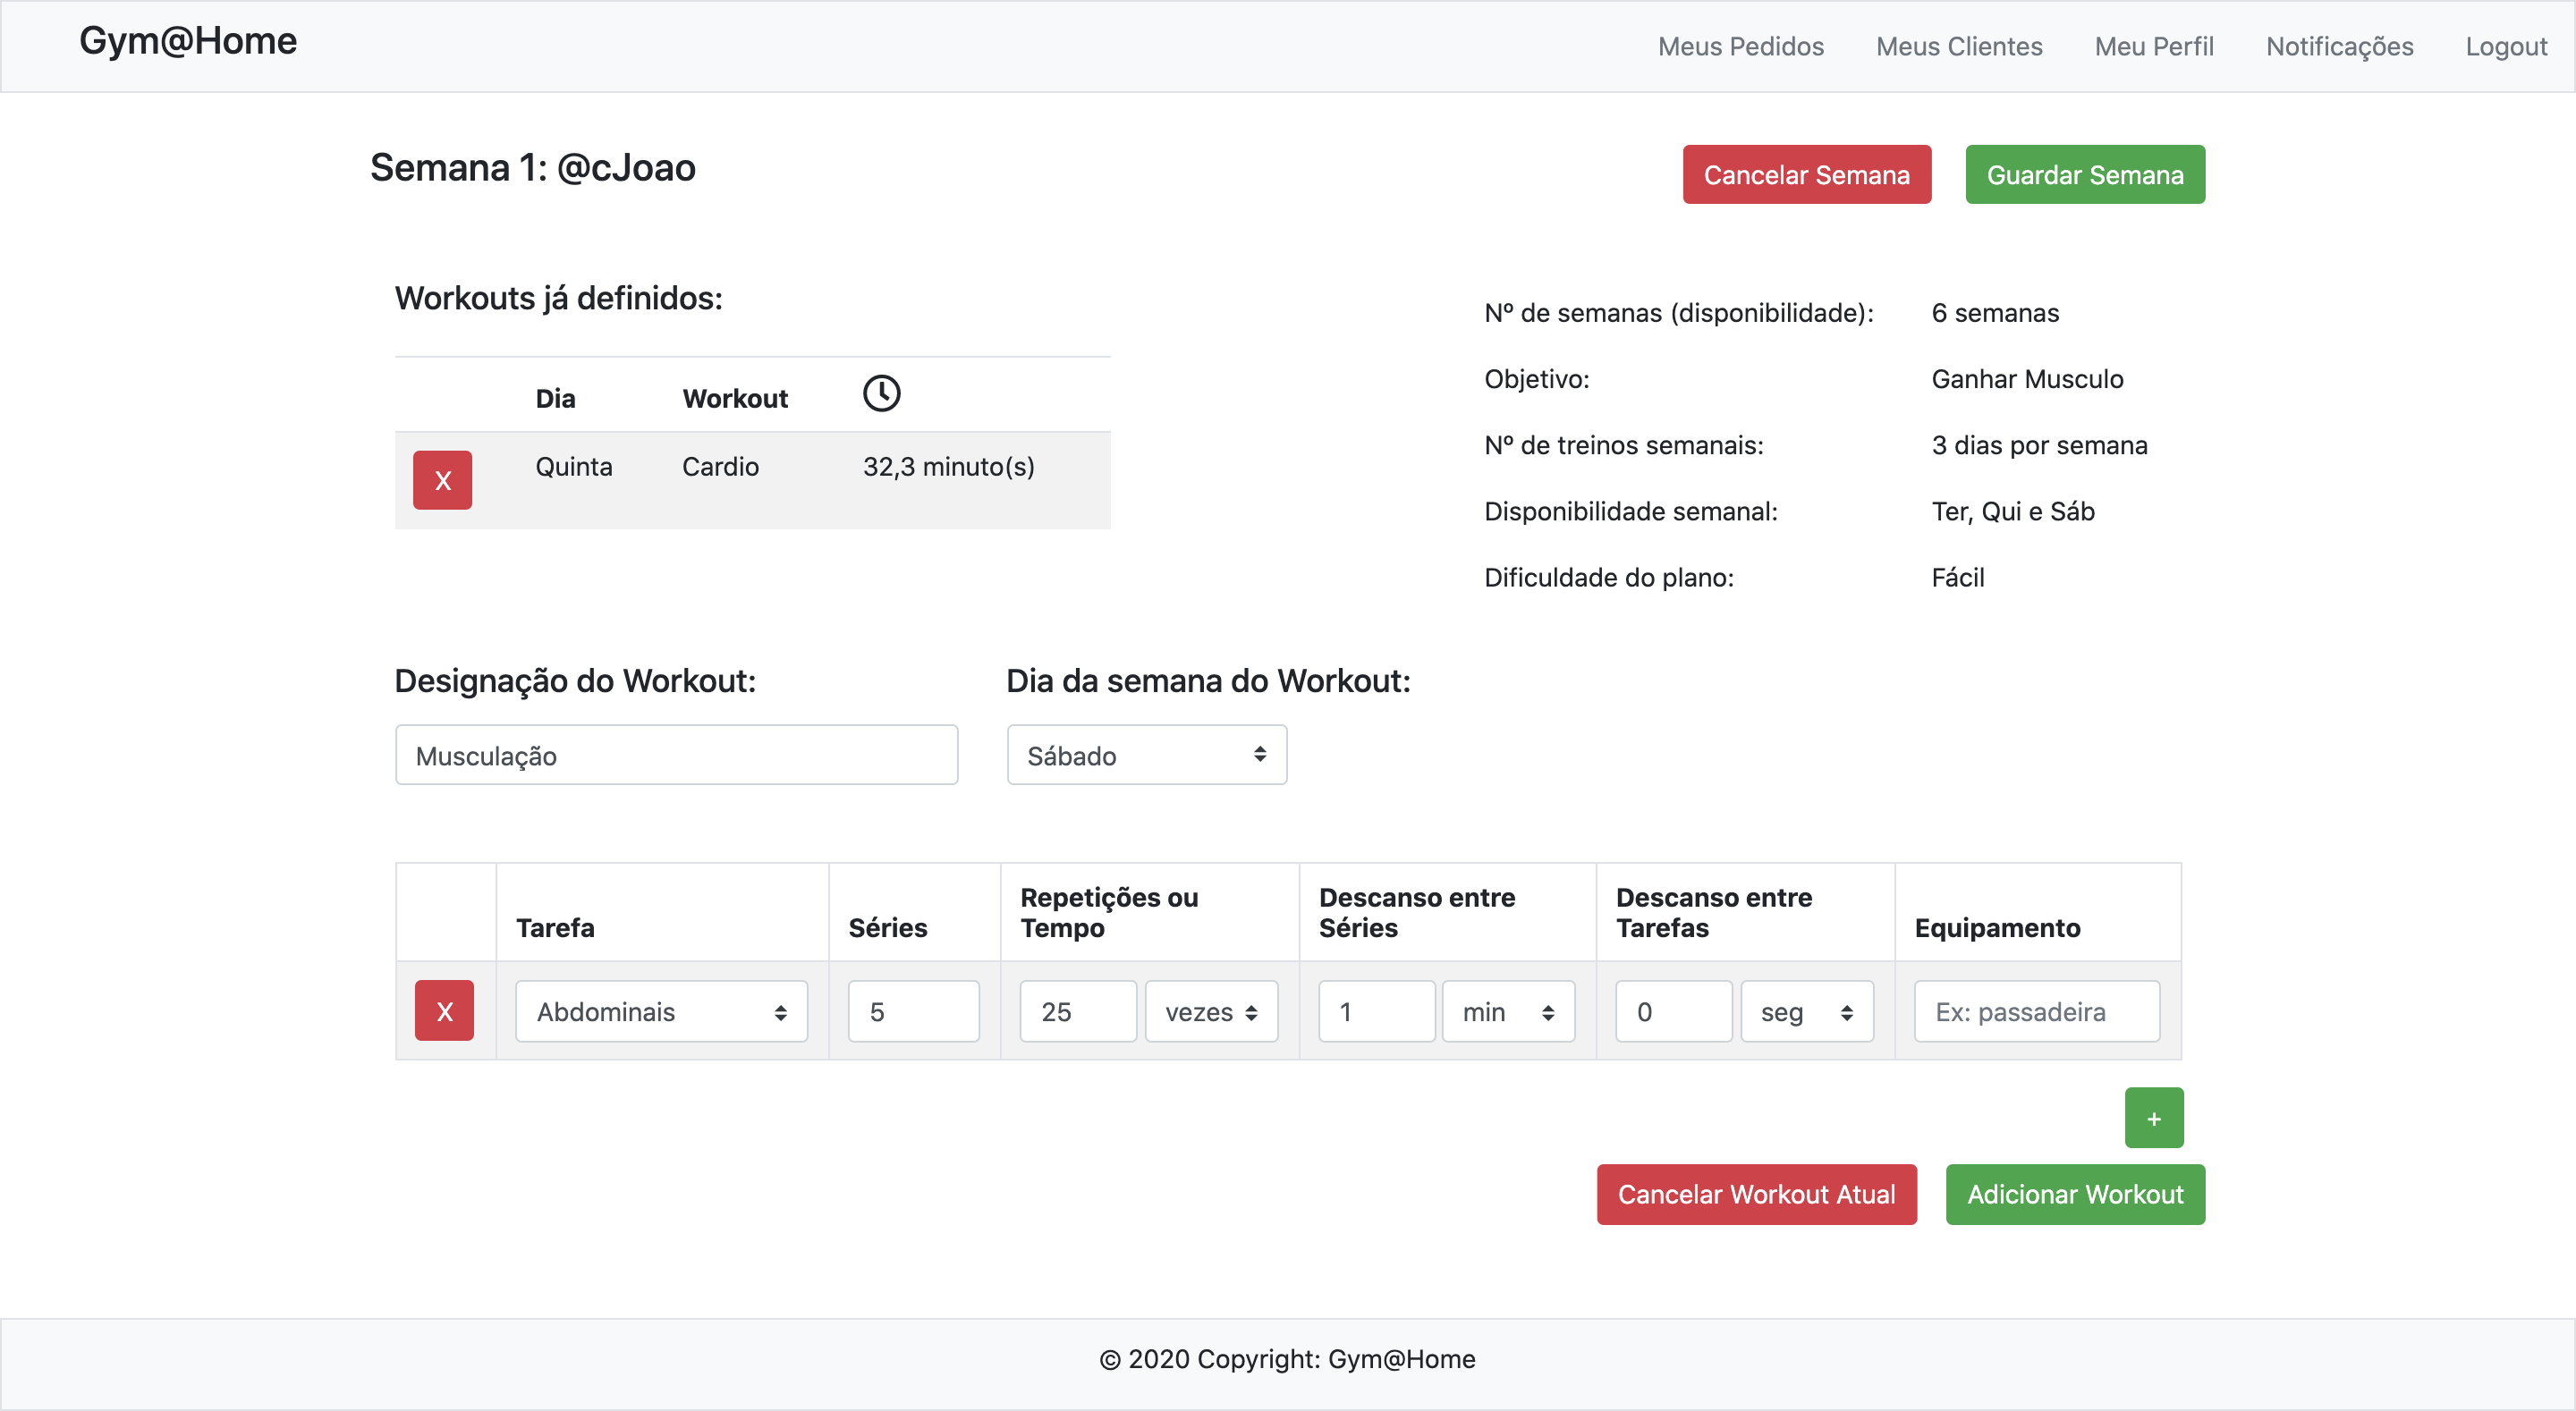
\includegraphics[scale=0.25]{images/interfaces/pt_criar_semana.png}
    \caption{Interface Criar Semana.}
    \label{fig:interfacecriarsemana}
\end{figure}

\subsubsection{Princípios de usabilidade}
\begin{itemize}
    \item \textbf{Substitutivity}: O PT pode definir um tempo em segundos ou em minutos.
    \item \textbf{Customizability}: pois o PT pode adicionar/remove mais linhas à tabela onde define as tarefas de um workout
    \item \textbf{Observability}: na medida em que, quando o PT guarda um workout, o mesmo faz \textbf{preload} na tabela que está no topo (tabela denominada, "wrokouts já definidos", podendo o mesmo observar os workouts que já definiu.
    \item \textbf{Recoverability}: a tabela onde estão os workouts já definidos permite apagar, ou seja, reverter. De modo semelhante, o botão "Cancelar workout" também reverte a tabela onde se define as tarefas.
\end{itemize}

\subsubsection{Heurísticas de Normam}
\begin{itemize}
    \item \textbf{Recognition rather than recall}: Os dados do pedido do Cliente são ilustrados durante a criação da semana para o PT não ter de se lembrar de quais eram os requisitos do pedido.
    
    \item \textbf{Error prevention}: Todos os inputs numéricos aceitam apenas números. Não é permitido ao PT "Guardar Semana" se a Semana não tiver nenhum Workout criado para a mesma.
\end{itemize}

\subsection{Semana do Cliente vista pelo PT}
\label{subsec:semanacliente}

\subsubsection{Descrição}
\hspace{5mm} A mockup é completamente análoga à "Semana" vista pelo Cliente, a única diferença é que no PT aparece o nome do Cliente ao qual aquela Semana pertence.

\begin{figure}[H]
    \centering
    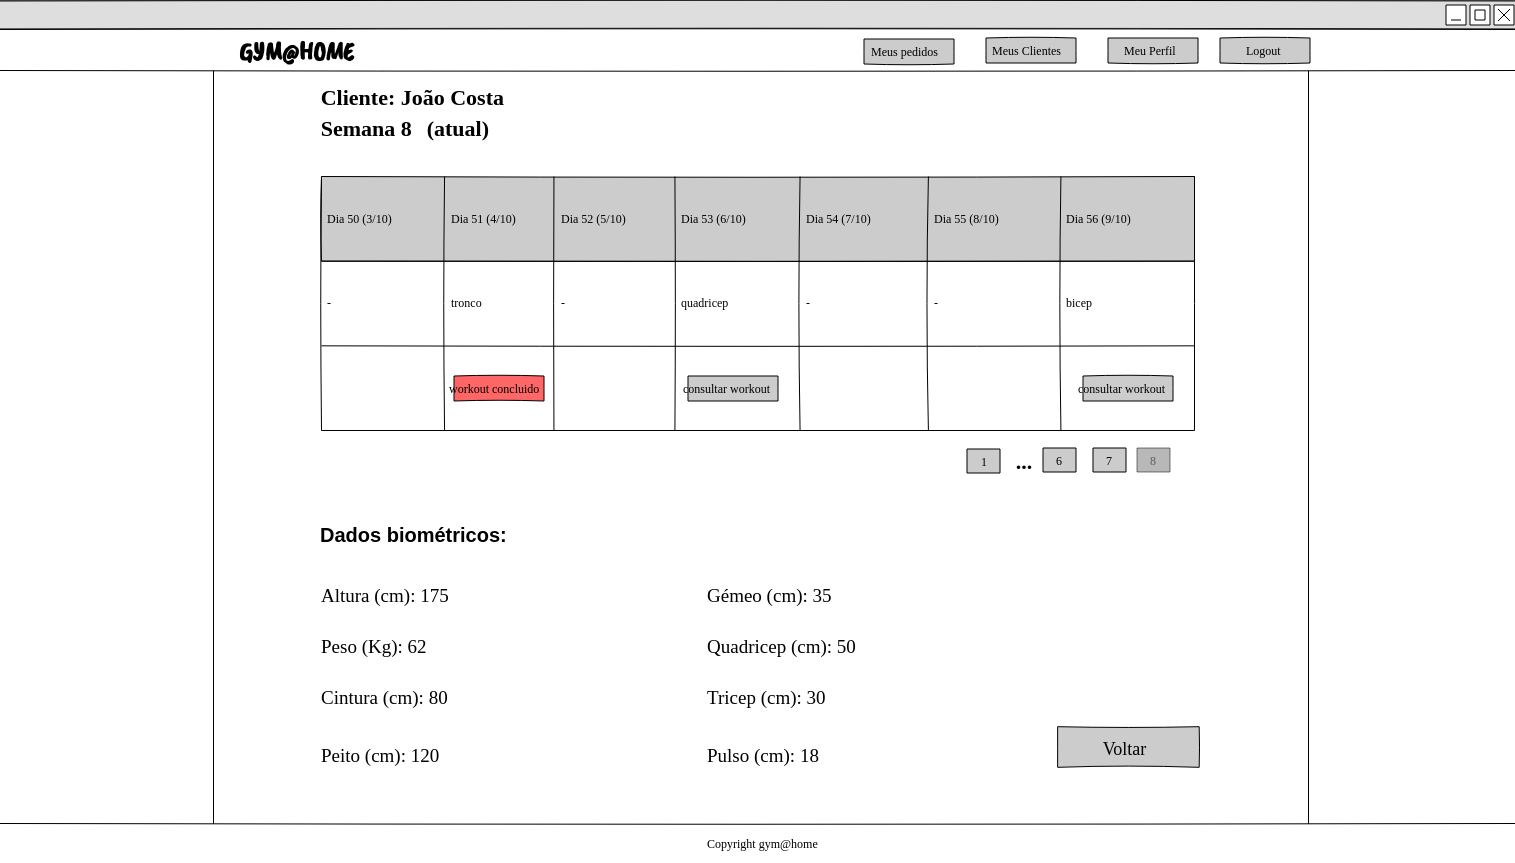
\includegraphics[scale=0.25]{images/mockups/pt_plano_do_cliente_semana_8_atual.png}
    \caption{Mockup Semana Cliente.}
    \label{fig:mockupsemanacliente}
\end{figure}

\begin{figure}[H]
    \centering
    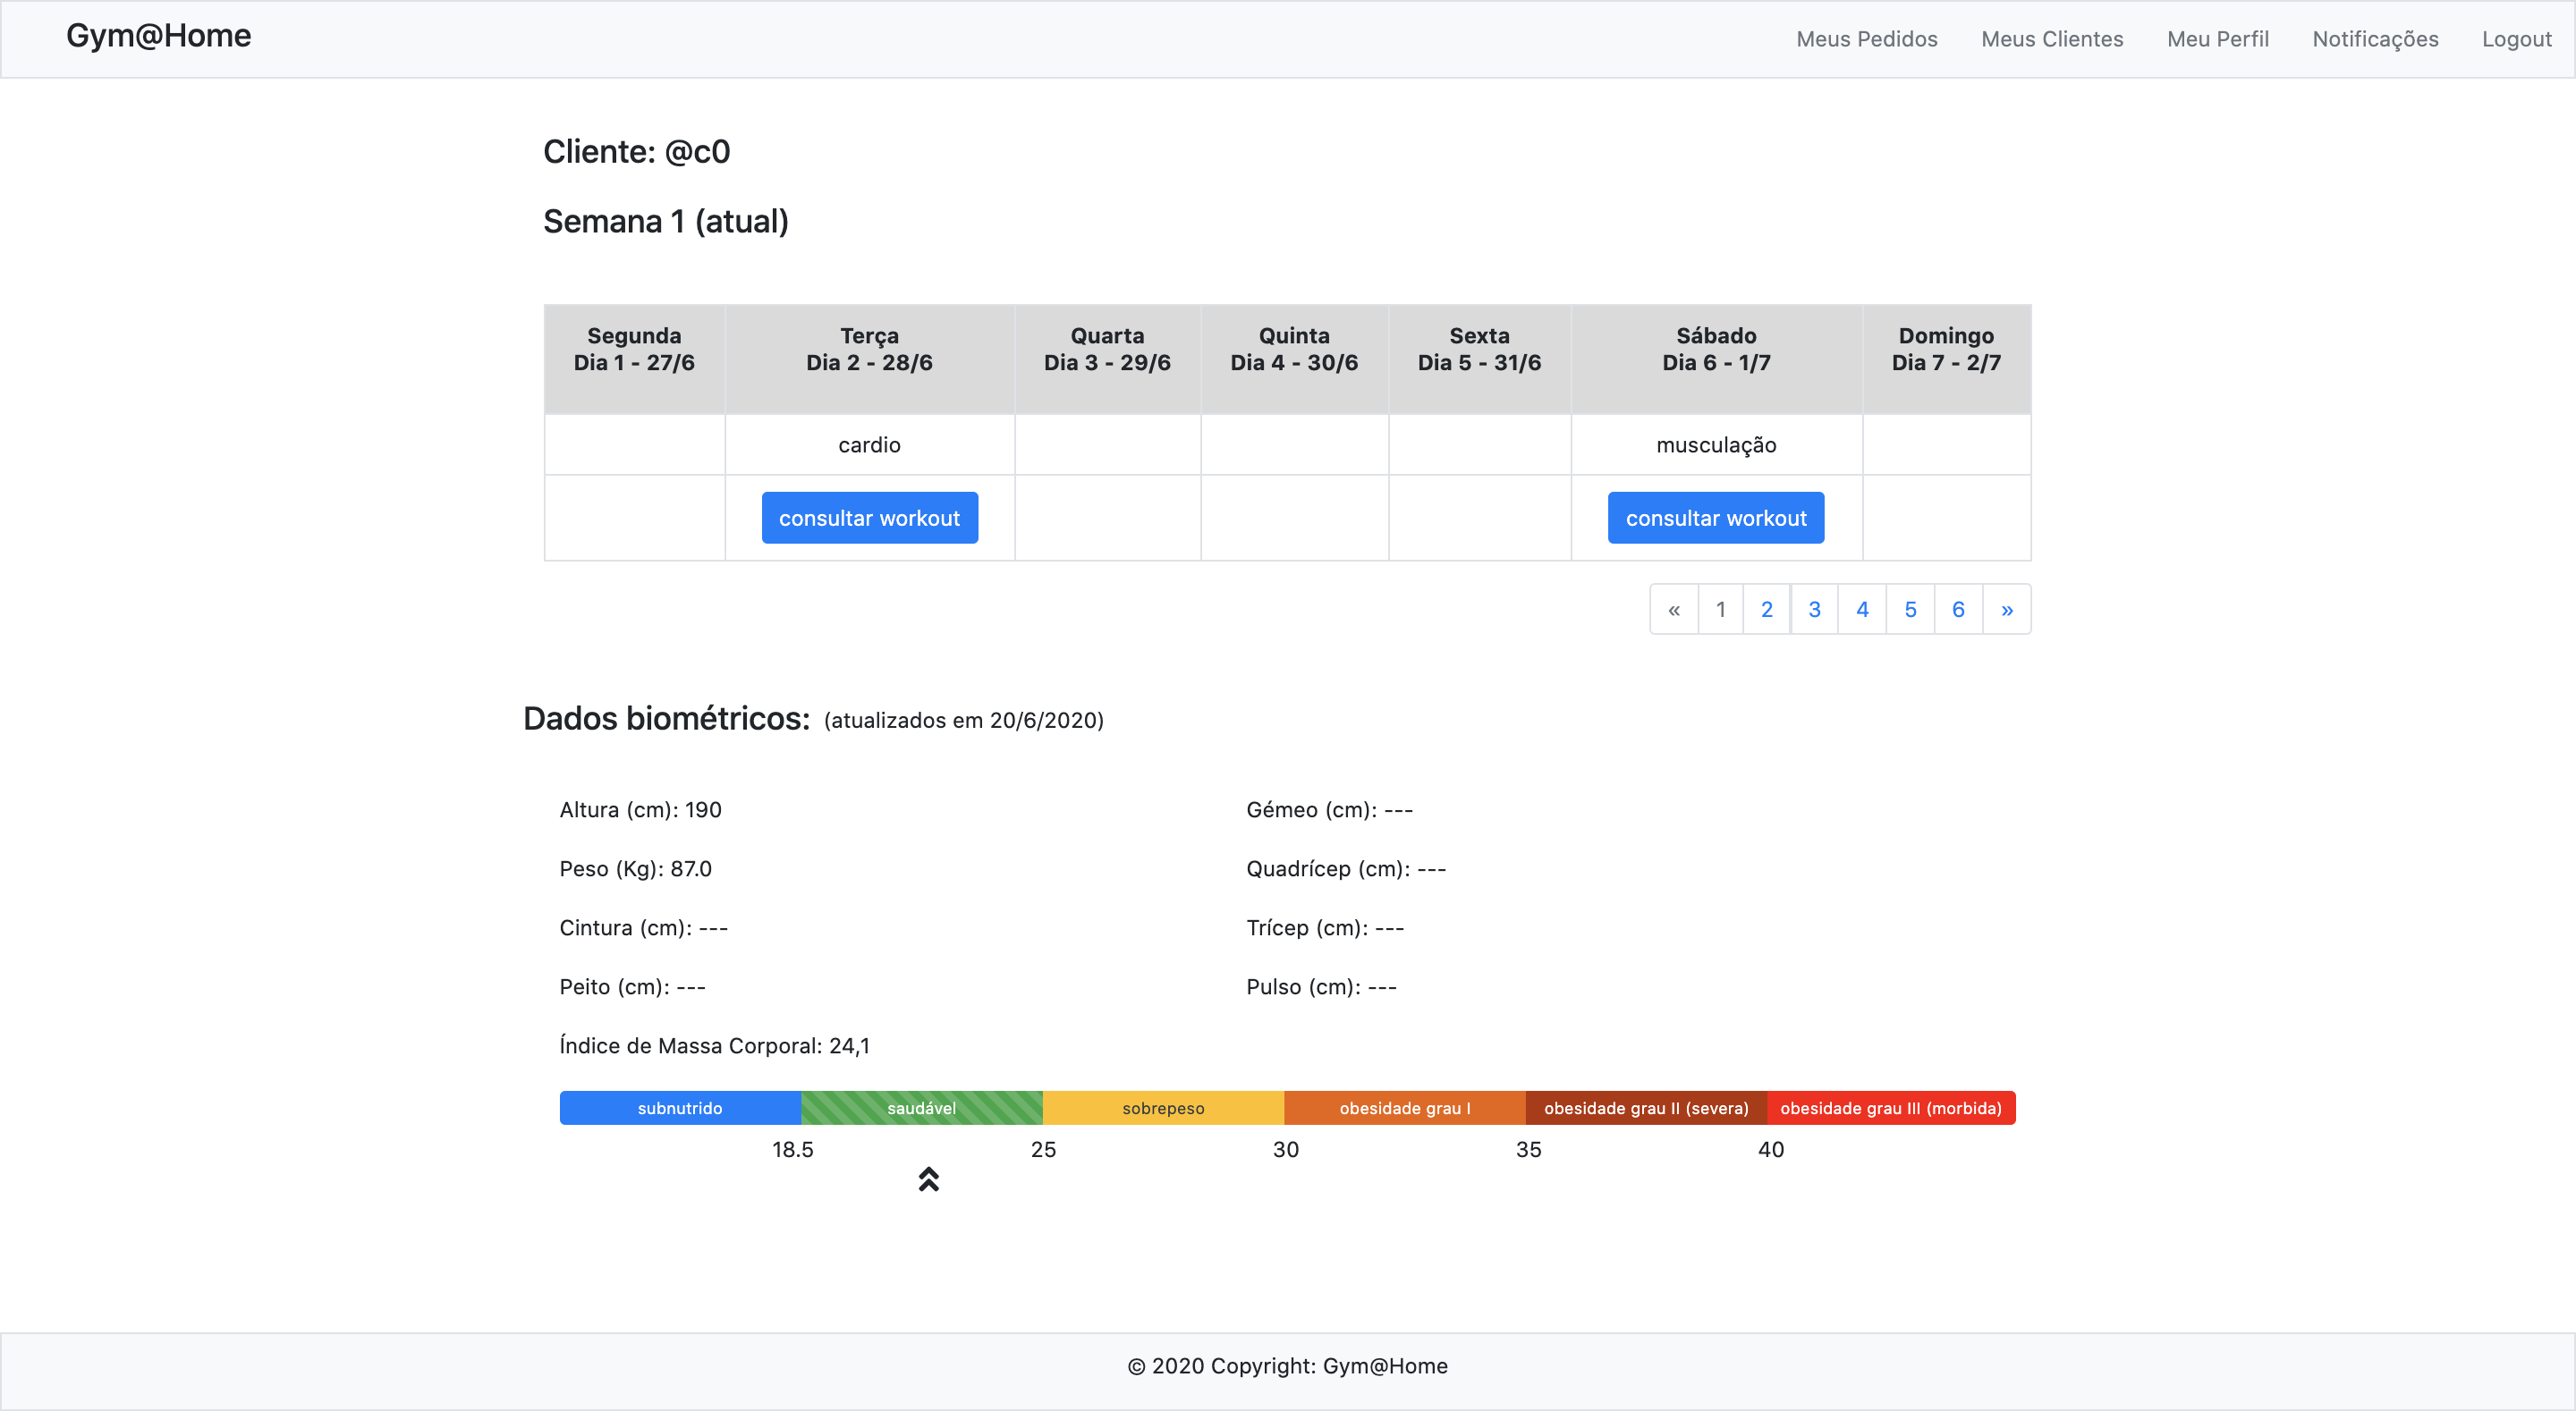
\includegraphics[scale=0.25]{images/interfaces/pt_semana.png}
    \caption{Interface Semana Cliente.}
    \label{fig:interfacesemanacliente}
\end{figure}

\subsubsection{Princípios de Usabilidade}
\begin{itemize}
    \item \textbf{Observability}: Mais especificamente \textbf{Browsability} pois o PT consegue navegar entre as várias semanas do plano do Cliente.
    
    \item \textbf{Familiarity}: utilizou-se o formato semanal \textbf{comum/padrão} em horários e calendários, visto que é mais familiar aos utilizadores.
    
    \item \textbf{Generalizability} e \textbf{Consistency}: visto que utilizou-se a mesma estrutura tanto para a consulta pelo PT, bem como pelo Cliente, apesar de terem algumas diferenças, manteve-se a estrutura semanal, bem como os dados biométricos, excepto o botão de avaliação do PT, que não faz sentido no lado do PT.
\end{itemize}

\subsubsection{Heurísticas de Normam}
\begin{itemize}
    \item \textbf{Recognition rather than recall}: Os dados biométricos do Cliente são ilustrados durante a visualização da semana para o PT não ter de se lembrar de quais eram os valores dos dados biométricos.
\end{itemize}

\subsection{Workout do Cliente visto pelo PT}
\label{subsec:workoutcliente}

\subsubsection{Descrição}
\hspace{5mm} Tal como na mockup anterior esta é totalmente análoga à do Cliente, sendo que nesta aparece o nome do Cliente e o \textbf{PT não pode finalizar Workout}.

\begin{figure}[H]
    \centering
    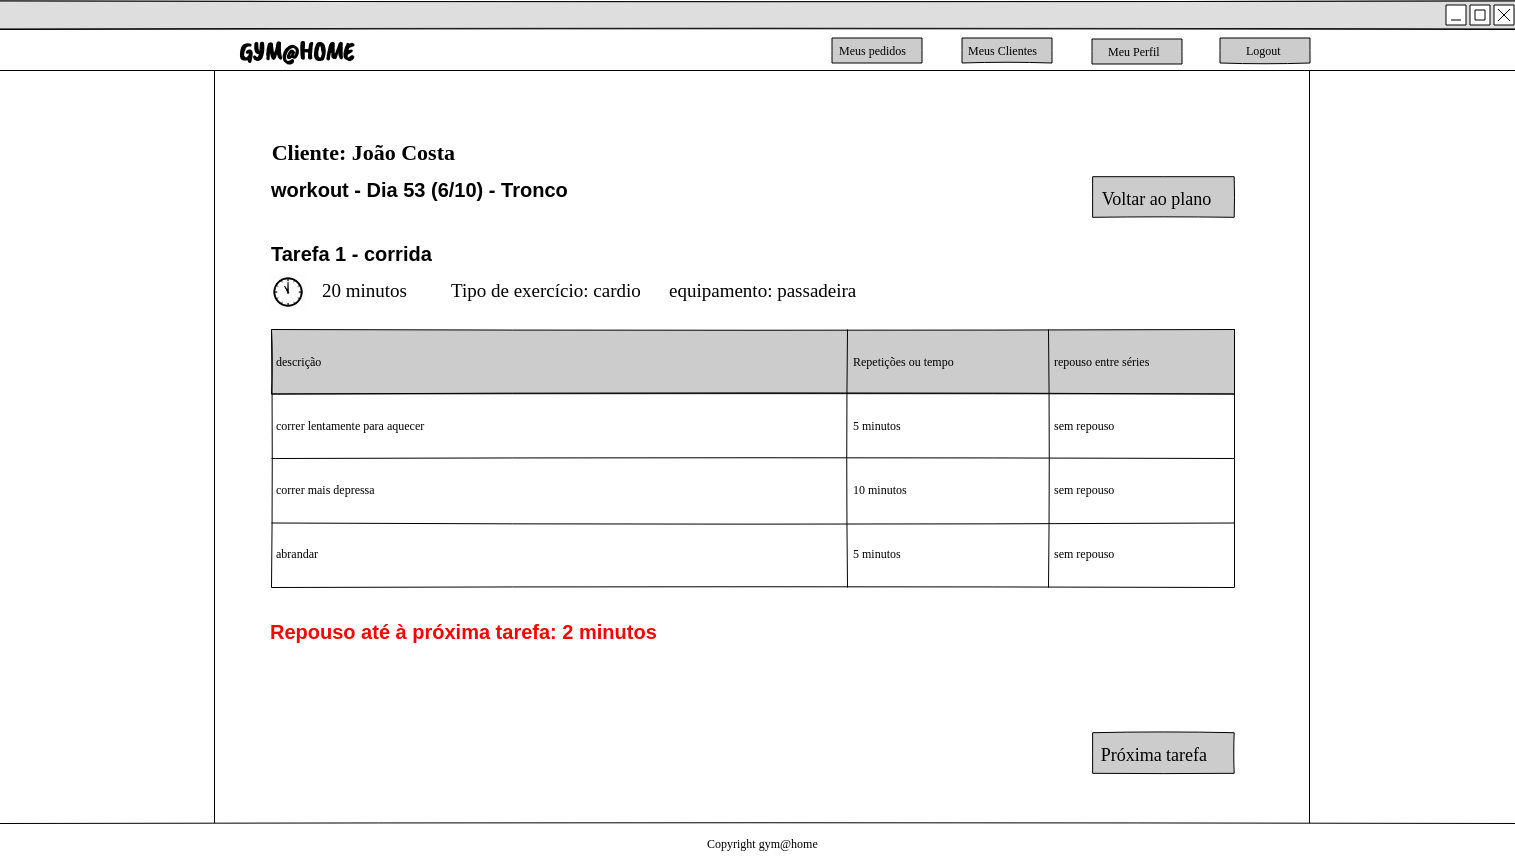
\includegraphics[scale=0.25]{images/mockups/pt_plano_do_cliente_tarefa_1.png}
    \caption{Mockup Workout Cliente.}
    \label{fig:mockupworkoutcliente}
\end{figure}

\begin{figure}[H]
    \centering
    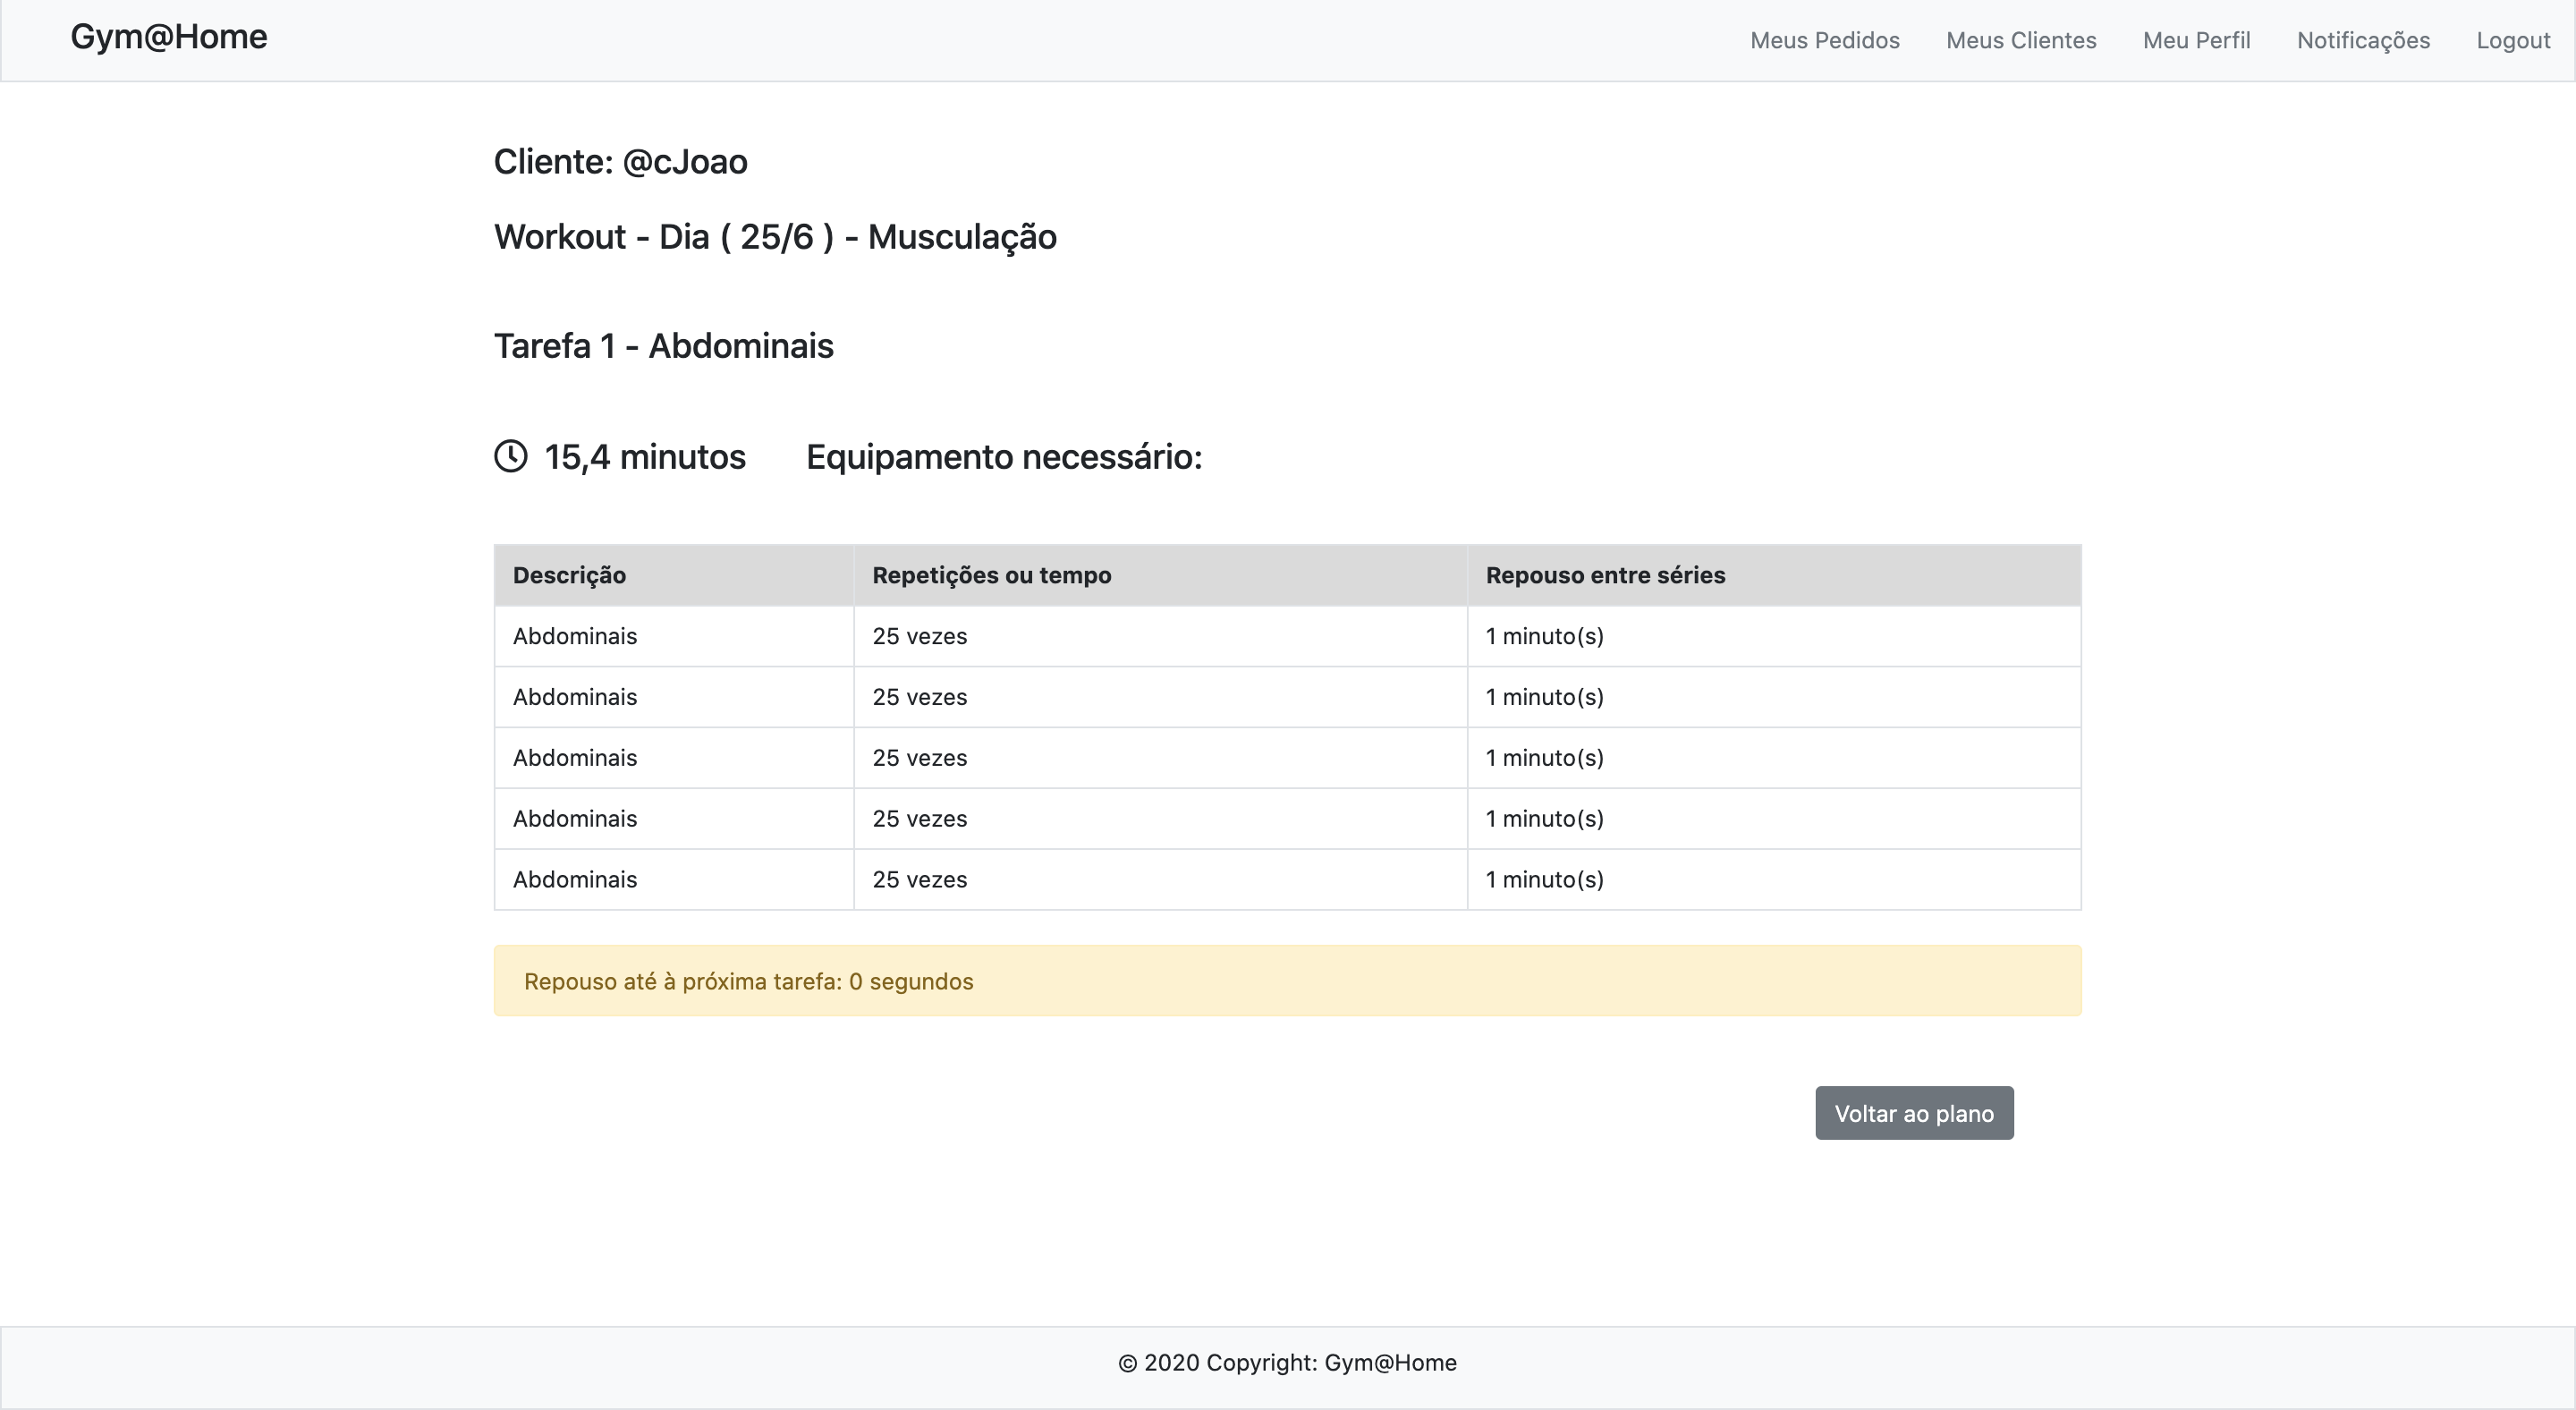
\includegraphics[scale=0.25]{images/interfaces/pt_workout.png}
    \caption{Interface Workout Cliente.}
    \label{fig:interfaceworkoutacliente}
\end{figure}

\subsubsection{Princípios de usabilidade}
\begin{itemize}
    \item \textbf{Observability}: Mais especificamente \textbf{Browsability} pois o PT consegue navegar entre as várias tarefas de um workout.
    
    \item \textbf{Generalizability} e \textbf{Consistency}: visto que utilizou-se a mesma estrutura tanto para a consulta pelo Cliente, bem como pelo PT, apesar de terem algumas diferenças, manteve-se a estrutura tabelar das séries de uma tarefa, bem como as informações da tarefa, considerando-se assim que torna-se genérica para ambos os utilizadores.
\end{itemize}

\subsubsection{Heurísticas de Normam}
\begin{itemize}
    \item \textbf{Recognition rather than recall}: as informações sobre o dia da semana e a definição do workout são passadas para esta view para que o cliente/PT não necessitem de memorizar.
\end{itemize}

%--------------------------------------------------------------------------%

\section{Alertas}
\label{sec:alertas}

\hspace{5mm} Algumas acções são impossíveis de reverter, dessa forma, deve-se dificultar as mesmas. Assim, foi criado o alerta de \textbf{confirmação} para ter a certeza que o utilizador pretende executar a acção.

\begin{figure}[H]
    \centering
    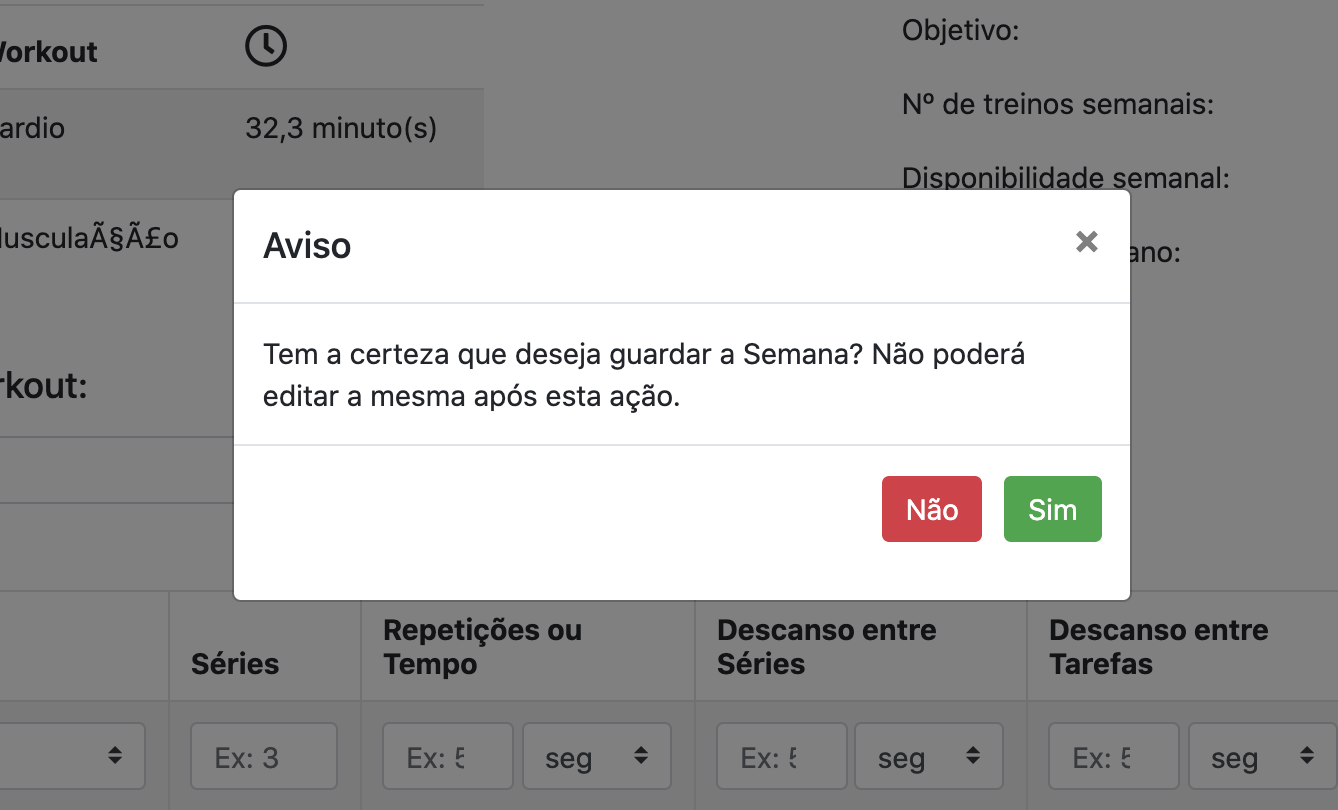
\includegraphics[scale=0.45]{images/alerts/alerta_confirmacao.png}
    \caption{Alerta de Confirmação.}
    \label{fig:alertaconfirmação}
\end{figure}